\chapter{Wavefront Control at LIGO Hanford}\label{chapter:MM_LHO}
	Simulations and calculations are wonderful guides to understanding and building intuition about mode matching, however, no model is perfect and experiments have a way of presenting the most interesting and challenging problems.  Preparation for the third observing run (O3) required extensive work to understand Advanced LIGO's path to achieve higher arm power.  One of the most important tasks was tuning the thermal compensation and interferometer sensing/controls systems in order to maintain the power build-ups in the PRC and arms during nominal low noise operation.  This chapter will build some constructs on how lensing affects the interferometer fields and a few strategies to tune the Thermal Compensation System (TCS) at LIGO Hanford. Then, summarizing in-situ measurements that were taken to understand the mode matching between the squeezer optical parametric oscillator (OPO) and the output mode cleaner in single bounce configuration
	
	For Advanced LIGO, test mass heating comes from main two sources: absorption by arm cavity optics from the main interferometer beam and effects of TCS which are meant to combat the wavefront distortion by applying heat in key places.  Thermal compensation currently utilizes ring heaters at all four main test masses, a disk heater at the SR3, and CO2 lasers at the input test masses.
	
	\section{Hot vs. Cold Interferometers}\label{sec:hotcoldifo}
	When fully operational, the arm cavities can have approximately 150 kilowatts of circulating power. An estimated but useful description of the total arm power in each arm is
	\begin{equation}
		P_{\text{ARM}} \approx \frac{1}{2} (g_{\text{PRC}} * g_{\text{ARM}} * P_{\text{in}})
	\end{equation}
	where $g_{\text{PRC}} \approx 45$ is the power recycling cavity gain and $g_{\text{ARM}} \approx 225$ is the single arm cavity gain. For O3, the intended input power $P_{\text{in}}$ will reach approximately 30 W which means $P_{\text{ARM}} \approx 150,000$ W. A fraction of that power between 0.2-0.8 PPM, will be absorbed by the high reflectivity surface creating a \textit{thermo-elastic} effect which changes the radius of curvature. By changing the test mass curvatures, the resonant Gaussian mode will also change its profile. Additionally, the \textit{thermo-refractive} effect will vary the index of refraction within the bulk as a function of absorbed temperature which creates at thermal lens that turns out to be an order of magnitude larger than the wavefront distortion from therm-elastic effects in fused silica \cite{winkler_thermaldist}.
	
	\subsection{Thermal Lensing}\label{Sec:TL_lensing}
	As seen in Section \ref{sec:DRMI}, the sideband and carrier frequencies propagate differently in the interferometer by design, which means their fields see different thermal lensing effects.  The ITM substrate which sees the thermo-refractive change from absorption will play the largest role because the carrier is not affected to first order, this will be shown in Section \ref{Sec:carrier_lensing}. To understand how the fields change, the easiest way is to invoke the ABCD transfer matrix approach to track how the phase changes as they propagate through the optical system \cite{Lawrence_TCS}.
	
	\begin{figure}[ht!]
		\centering
		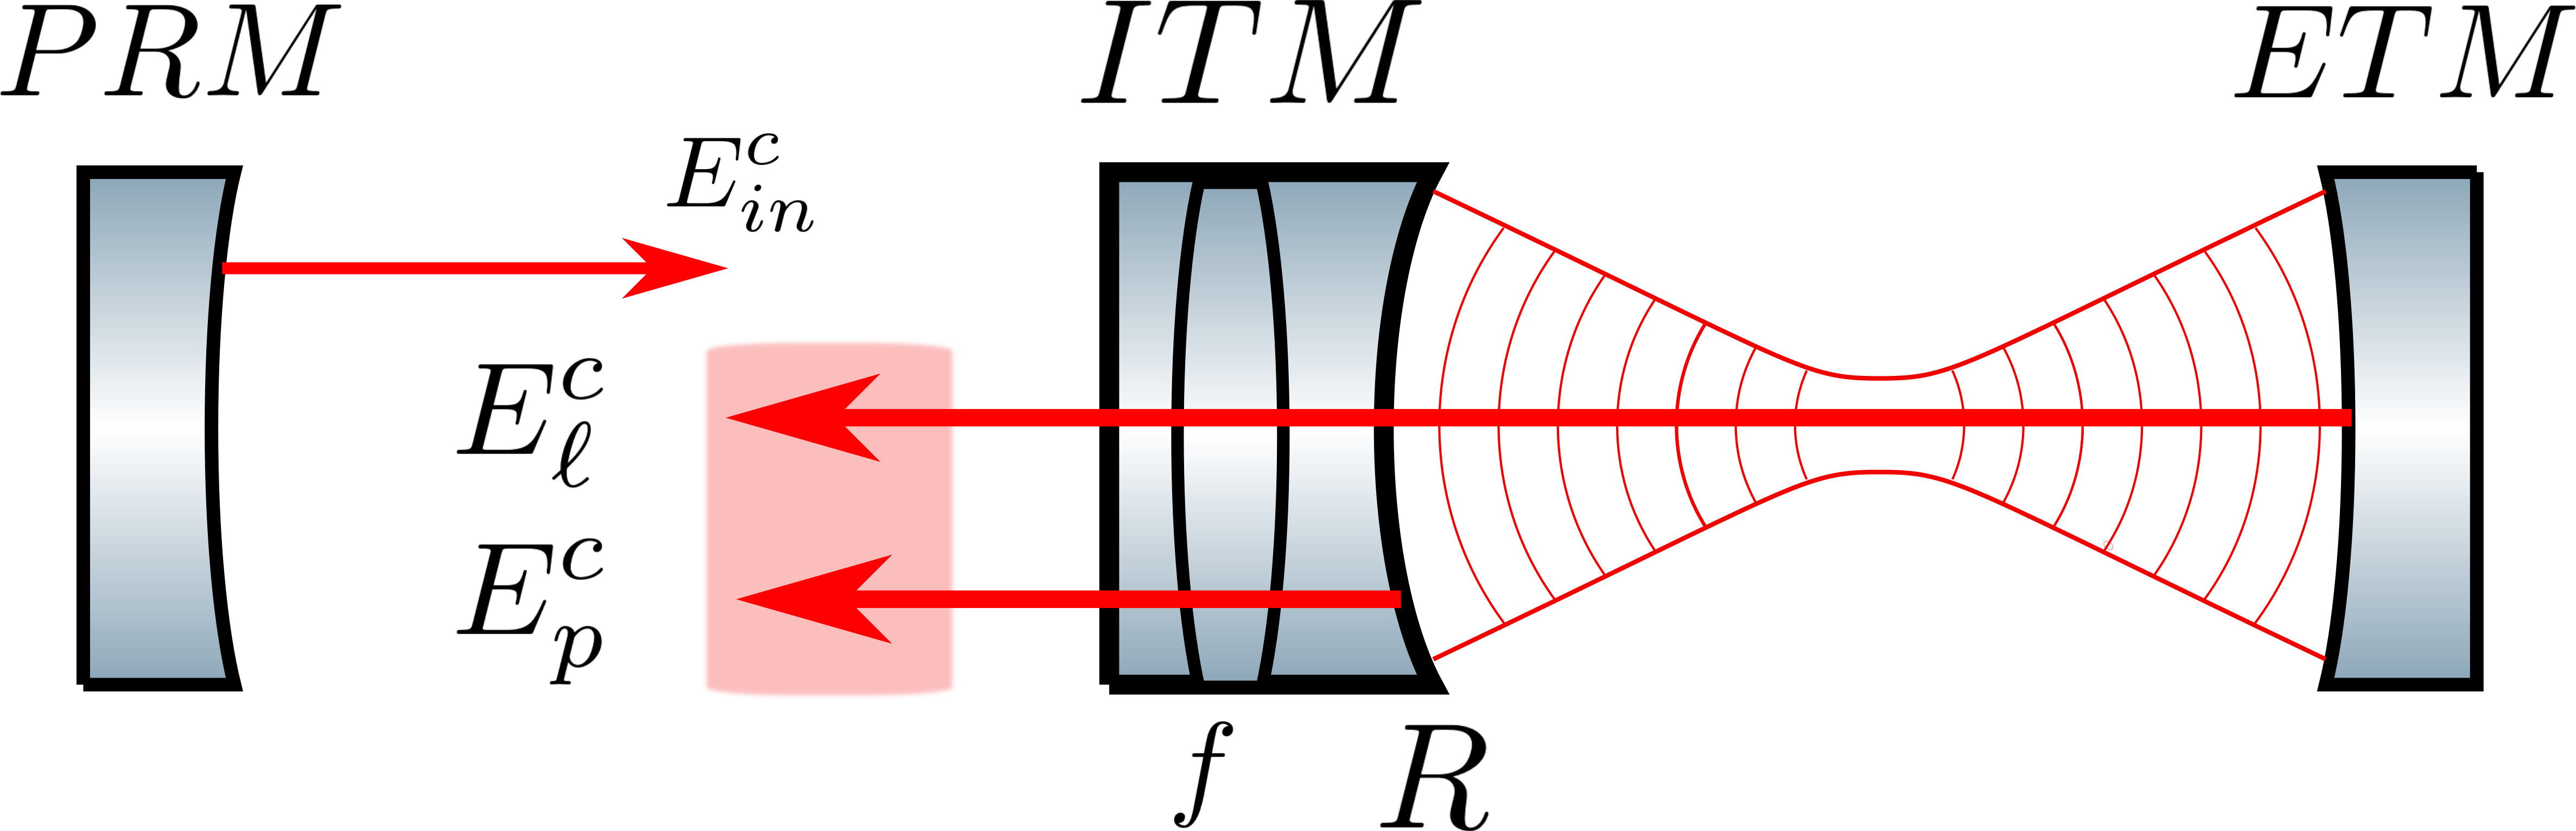
\includegraphics[width=.7 \textwidth]{../Figures/ThermalLensFP.png}
		\caption[A simplified model for the effect of a substrate thermal lens on the carrier field.]  
		{\textbf{A simplified model for the effect of a substrate thermal lens on the carrier field.} An input beam, $E_{\text{in}}^{c}$, from the power recycling mirror (PRM) will have a radius of curvature that mode matches to the input test mass (ITM).  The promptly reflected beam, $E_{p}^{c}$, is denoted by equation \ref{eq:promptE} and the leakage beam, $E_{\ell}^{c}$, is expressed by equation \ref{eq:leakE} where the sum of them would make the total reflected beam.  The leakage field will have the same shape as the ITM radius of curvature $R$ when exiting the arm and see the thermal lensing $f$. The promptly reflected field will also see the lens $f$ twice but when combined with the leakage beam, the \textit{total} reflected field is not affected by the thermal lens.}
		\label{fig:ThermalLensFP}
	\end{figure}
		\subsubsection{Carrier}\label{Sec:carrier_lensing}
		The carrier is resonant in the 4 kilometer arm cavities as well as the PRC, so a simplified model resembles a coupled cavity setup where there is already a locked resonator with some leakage beam and there is an input mode propagating from the power recycling cavity.  Consider the diagram in Figure \ref{fig:ThermalLensFP}, a two-mirror optical system which has an input carrier beam, $\ket{E^c_{\text{in}}}$, that has a portion promptly reflected off the input mirror to create $\ket{E^c_{p}}$
		\begin{equation}
		\ket{E^{c}_{p}} = \hat{M}^{c}_{p} \ket{E^{c}_{\text{in}}}
		\end{equation}
		The prompt reflection is made up of a beam incident on a converging lens(-) from the substrate and a single reflection from the input coupler's convex(+) surface, therefore, the transfer matrix is
		\begin{equation}
		\hat{M}^{c}_{p} = 
		\begin{bmatrix}
						1 	&	0 
		\\ 	-\frac{1}{f} 	&	1
		\end{bmatrix}
		\begin{bmatrix}
						1 	&	0 
		\\ 	+\frac{2}{R} 	&	1
		\end{bmatrix}
		\begin{bmatrix}
						1 	&	0 
		\\ 	-\frac{1}{f} 	&	1
		\end{bmatrix}
		\end{equation}
		where $R$ is the radius of curvature of the high reflectivity surface and $f$ is the focal length of the mirror substrate. In general, this can be a combination of the static lens and any thermal effects which create additional (intentional or non-intentional) lensing.
		
		\begin{equation}\label{eq:promptE}
		 \ket{E^{c}_{p}}=
		 \hat{M}^{c}_{p}
		 \begin{bmatrix}
		 					1  
		 \\ 	\frac{1}{q_{\text{in}}}
		 \end{bmatrix}
		 =
		 \begin{bmatrix}
		 1  
		 \\ 	\frac{1}{q_{\text{in}}} + 2 \big(\frac{1}{R} - \frac{1}{f}\big)
		 \end{bmatrix}
		 =
		 \begin{bmatrix}
		 1  
		 \\ 	\frac{1}{q_{\text{p}}}
		 \end{bmatrix}
		\end{equation}
		
		In addition, there is also a circulating field inside the cavity which leaks out in reflection and can be denoted by $\ket{E^c_{\ell}}$ which exits with the input coupler's radius of curvature and sees a single pass through the substrate lens,
		\begin{equation}\label{eq:leakE}
		\ket{E^c_{\ell}} = 		 
		\begin{bmatrix}
		1 	&	0 
		\\ 	-\frac{1}{f} 	&	1
		\end{bmatrix}
		\begin{bmatrix}
		1  
		\\ 	\frac{1}{R}
		\end{bmatrix}
		=
		\begin{bmatrix}
		1  
		\\ 	\frac{1}{R} - \frac{1}{f}
		\end{bmatrix}
		\end{equation}
		The total reflected beam is a summation of the prompt and leaked cavity fields.  LIGO uses arms which are highly over-coupled optical cavities so the promptly reflected amplitude is $\vert E^c_p \vert \approx \vert E_{\text{in}} \vert$ and using equation \ref{c_FP}, the leakage amplitude is $\vert E^c_\ell \vert \approx -2\vert E_{\text{in}} \vert$.  Putting all this together, the total reflected field of the carrier is
		\begin{equation}
		\begin{aligned}
		E^c_{\text{REFL}} 	&= E^c_{\ell} + E^c_p \\
							&= E_{\text{in}} \bigg[ \exp \bigg(\frac{-ik r^2}{2q_p}\bigg) - 2  \text{exp} \bigg(\frac{-ik r^2}{2q_{\ell}}\bigg) \bigg]\\
							&\approx E_{\text{in}} \bigg[ -1 - \frac{ikr^2}{2} \bigg( \frac{1}{q_p} - \frac{2}{q_\ell} \bigg) \bigg]\\
							&\approx -E_{\text{in}} \exp\bigg(\frac{ikr^2}{2q_{\text{in}}}\bigg) 
		\end{aligned} 
		\end{equation}
		This shows that the total reflected carrier field will be the original amplitude with a negative sign and the same absolute curvature, however, now the beam is diverging instead of converging.  \textbf{The amazing part is that the end result is independent of the substrate lensing to first order}.  The point where this model breaks down is when the power recycling mode is altered so much by lensing effects that the PRC is no longer well mode matched to the arms; this leads to the input beam not having the right radius of curvature.  At that point, there will be extra losses from higher order mode-coupling.  In addition, lensing can change the radius of curvature to a point where the PRC g-factor makes the resonant mode no longer geometrically stable (see Appendix \ref{FPappendix}), however, this requires significant thermal lensing well beyond what is expected in Advanced LIGO \cite{Lawrence_TCS}.  A numerical FINESSE model uses this simplified geometry to calculate the power recycling gain and arm build up in Figure \ref{fig:simple_prc_arm} as a function of round trip losses and thermal lensing.
		\subsubsection{Sidebands}
		Using the same formalism as the carrier fields, the sidebands will have the same input curvature, however, they do not resonate in the arms so there is no cavity leakage field.  Therefore, the sidebands will see the phase change due to the substrate lens and this has very important consequences on the sideband build up within the power recycling cavity.
		\subsubsection{GW Signal}
		As mentioned in Section \ref{sec:DRMI}, LIGO currently employs a DC readout scheme that extracts the signal by beating the carrier field with the audio frequency sidebands created by the gravitational wave.  Although the carrier field was shown to be immune from substrate thermal lensing, the gravitational wave sideband field will see a single-passed lensing effect as it propagates out of the cavity and towards the beamsplitter.  If there is differential lensing, the signal recycling cavity will see an effective thermal lens, $\text{TL}_{-}$, which will be scattered into higher order modes.  This reduces the amount of gravitational wave signal at the anti-symmetric port that is directly proportional to the mode mismatch between the arms.
		
	\section{Wavefront Distortions from Thermal Effects}\label{sec:wf_dist}
	In the previous section, it was shown that lensing in the substrate affects fields in the interferometer differently.  The thermal distortions were modeled as a simple addition of phase, however, it is useful to understand how the optical path varies from first principles.  This provides theoretical groundwork for modeling interferometer heating as well as corrective measures using TCS.  A lot of work in this field was introduced in the context of gravitational wave detectors by Hello and Vinet \cite{hello_vinet} \cite{Vinet_Thermal_Issues} where they implemented the Heat Diffusion equation in order to analytically derive the phase change due to thermal aberrations.  In general, there are two effects which occur when a beam interacts with an optic which has a temperature field: thermo-refractive and thermo-elastic.  
	
	The first arises from the index of refraction changing as a function of the temperature distribution $T(r,z)$,
	\begin{equation}
	\Delta n_{r}(r,z) = \frac{\text{d}n}{\text{d}T} \, T(r,z)
	\end{equation}
	where $\frac{\text{d}n}{\text{d}T}$ is the temperature index coefficient and is dependent on the optic material.  For example, if the heating source comes from a laser beam which imparts onto the optic a Gaussian-like intensity pattern, the temperature profile will be non-uniform and lead to a varying index of refraction that causes wavefront distortions (see Figure \ref{fig:ThermalLensWF}).
	
	\begin{figure}[ht!]
		\centering
		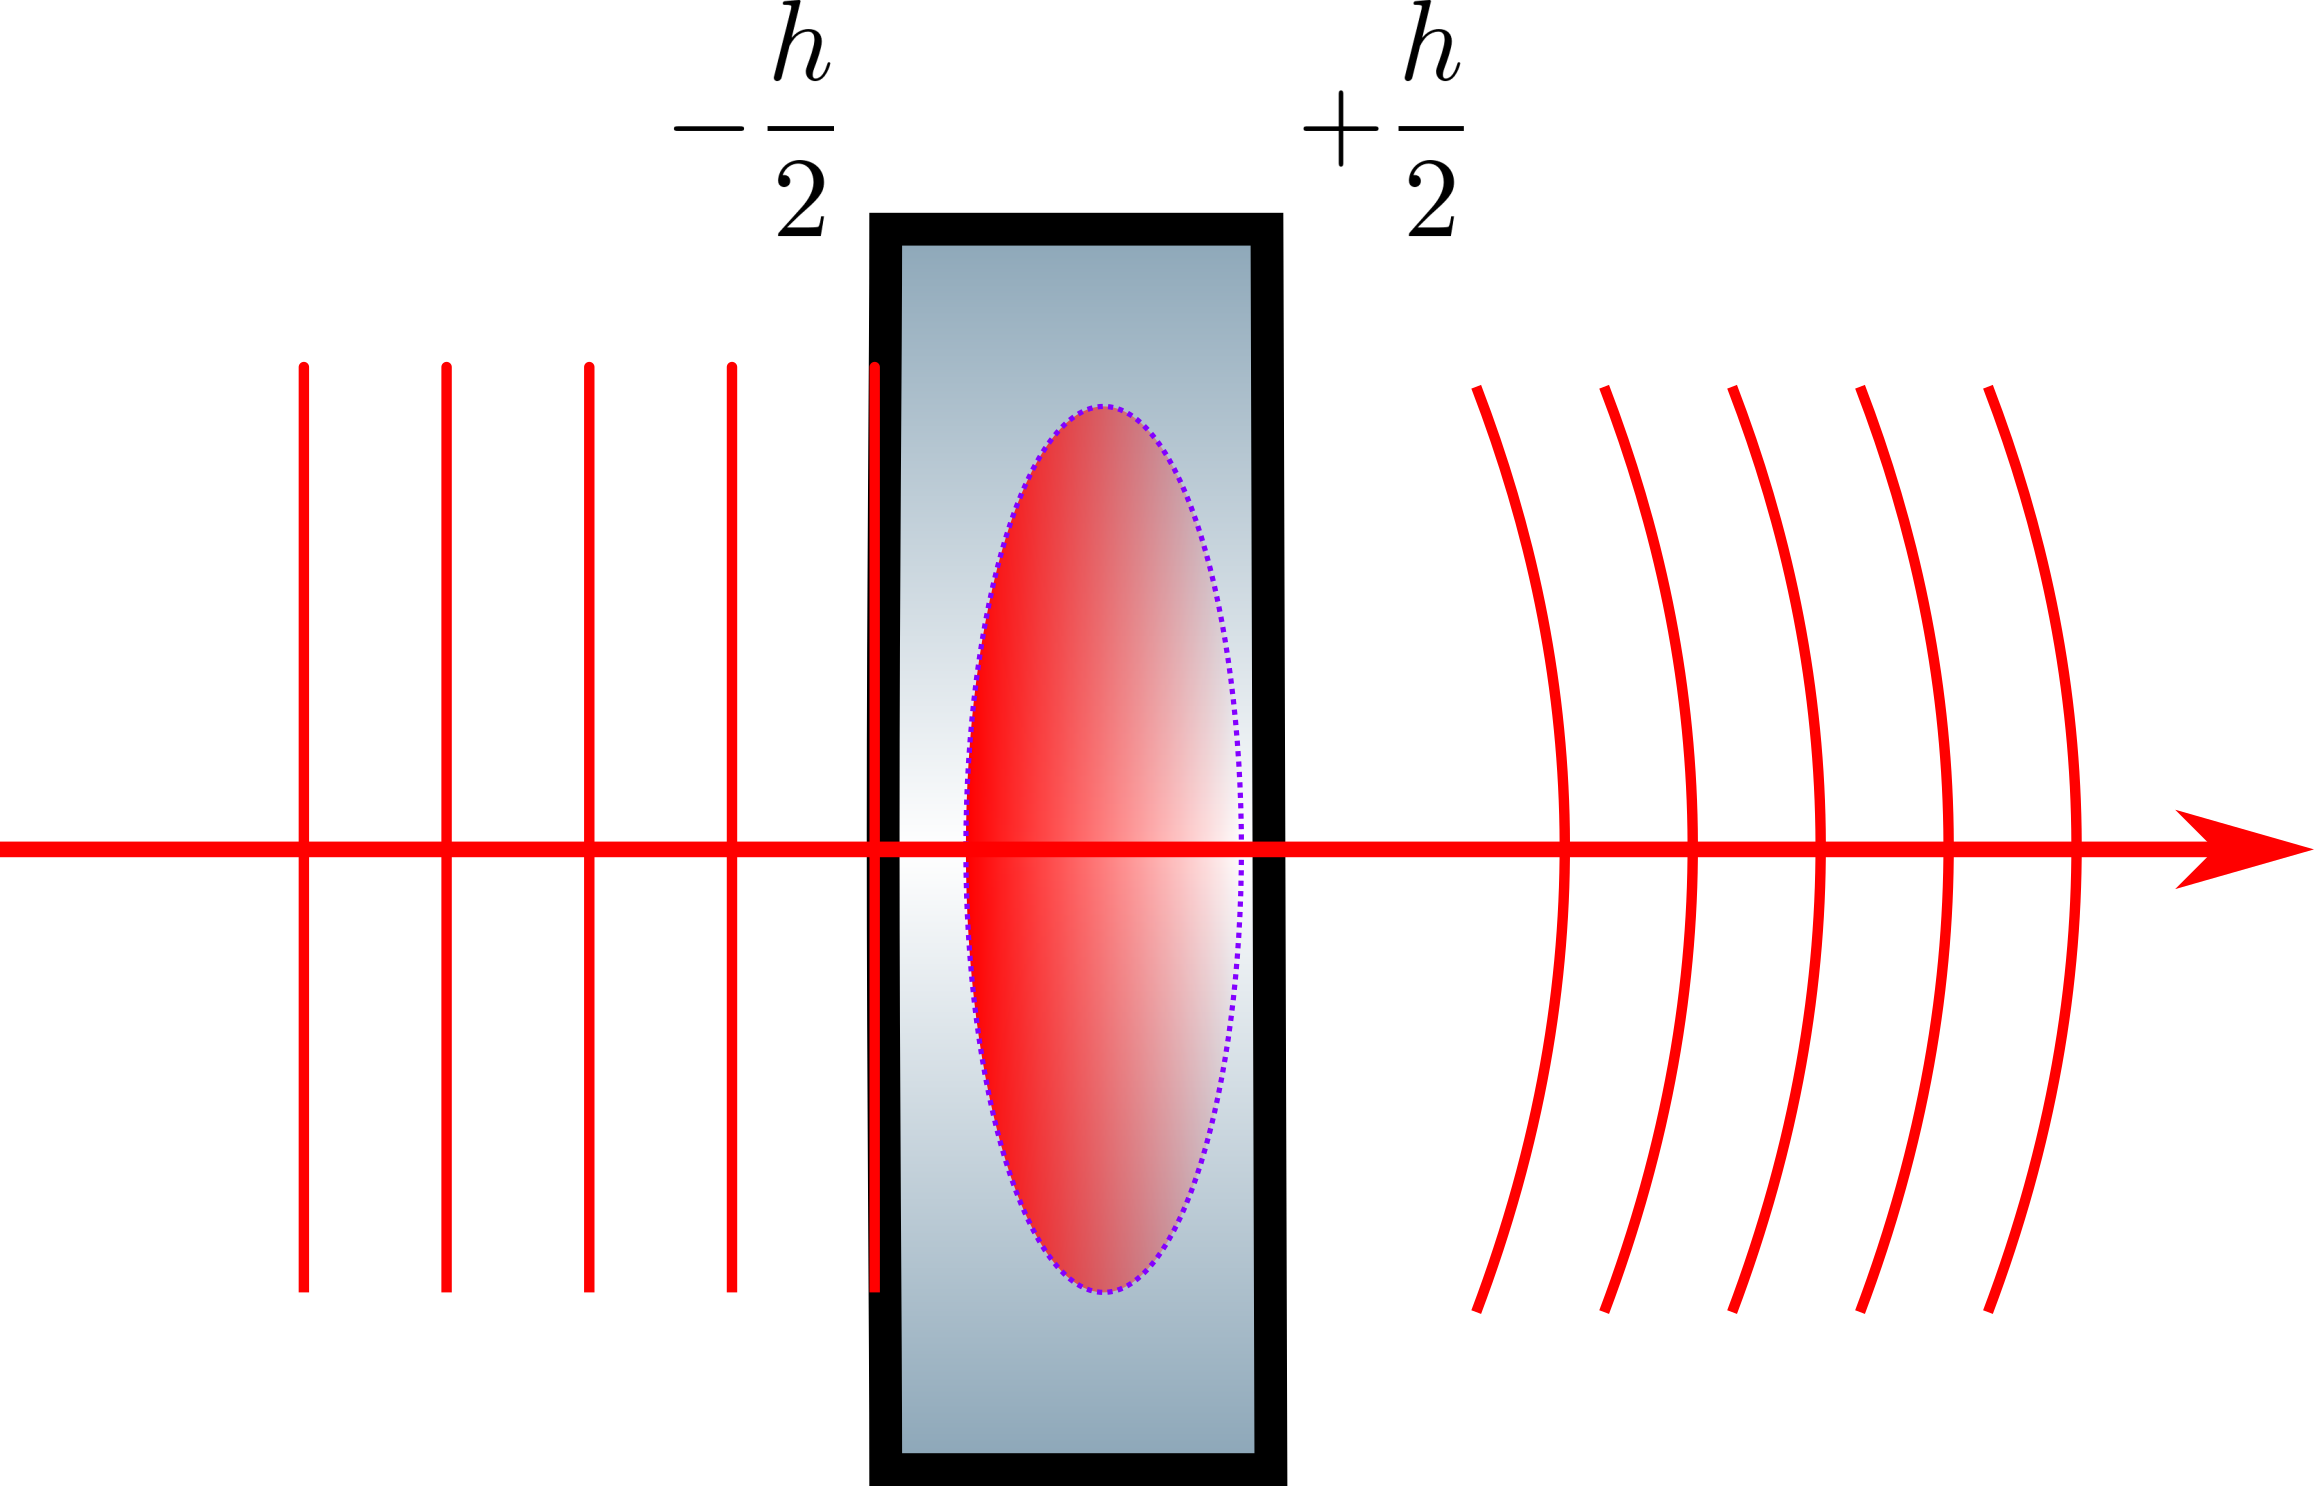
\includegraphics[width=.4 \textwidth]{../Figures/ThermalLensWF.png}
		\caption[A plane wave passing through a lens with a temperature gradient.]  
		{\textbf{A plane wave passing through a lens with a temperature gradient.} The index of refraction, $n$, depends on the material and temperature so when a plane wave moves through a medium with a non-uniform temperature field, a phase lag or lead occurs in the wavefront. Since $\frac{\text{d}n}{\text{d}T}$ is negative, the distortion will resemble a diverging lens.}
		\label{fig:ThermalLensWF}
	\end{figure}

	To understand how changing the index of refraction varies the optical path length, consider the function $S(r)$ which describes surfaces that are perpendicular to the rays. If $S(r)$ is a known function then the rays can be reconstructed using the gradient, $\nabla S(r)$.  As an analogy to electrostatics, $S(r)$ is similar to the potential function $V$ and the electric field is described by $\bf{E}=-\nabla V$.  As an extension of ray optics, Fermat's principle requires that the Eikonal equation be satisfied,
	\begin{equation}
	\vert \nabla S \vert^2 = n^2
	\end{equation}
	By integrating along the axis of propagation ($\hat{z}$) in Figure \ref{fig:ThermalLensWF} through the substrate, one can find the optical path distortion
	\begin{equation}\label{eq:thermoref}
	Z(r) =  \frac{\text{d}n}{\text{d}T} \int_{-h/2}^{+h/2} \, T(r,z) \text{d}z
	\end{equation}
	It is clear that the temperature field is key to understanding exactly how the wavefront is distorted. In order to analytically solve for $T(r,z)$, one must invoke the famous Heat equation,
	\begin{equation}\label{eq:heat_eq}
		\kappa \nabla^2 T(r,z) = \rho C\, \frac{\partial T}{\partial t} 
	\end{equation}
	where $\kappa$ is the thermal conductivity, $\rho$ is the density, and $C$ is the specific heat.  A complete solution for such an equation will be a sum of two parts: 
	\begin{equation}
	T(r,z,t) = T_{s}(r,z) + T_{t}(r,z,t)
	\end{equation} 
	where the first term is the steady-state solution which includes the an ambient temperature and a perturbation, $T_s(r,z) = T_p(r,z) + T_0$.  The main goal for the remainder of the section will be finding a solution to the perturbation field.  The second term is the transient time-dependent solution which will converge to the stead-state as time goes to infinity.  For the LIGO test masses which are approximately cylindrical, the heat equation in steady-state equilibrium is
	\begin{equation}
		\kappa \bigg[ \frac{1}{r} \frac{\partial}{\partial r} \bigg( r \frac{\partial}{\partial r}\bigg) +  \frac{\partial^2}{\partial z^2} \bigg] T_s(r,z) = 0
	\end{equation}
	The next step is to understand the boundary conditions using Figure \ref{fig:ThermalLensFlux} and the balance of heat fluxes at each of the surfaces,
	\begin{equation}
	\textbf{n} \cdot [ \textbf{F} + \kappa \nabla T_s]_{\text{surf}} = 0 
	\end{equation}
	Assuming that the outward flux is from radiation which follows the Stefan-Boltzmann law,
	\begin{equation}\label{eq:heat_flux}
	\begin{aligned}
	[\textbf{n} \cdot  \textbf{F}]_{\text{surf}} = \sigma_B  [T_s^4 - T_0^4] 	&= \sigma_B [(T_p(r,z) + T_0)^4 - T_0^4] \\
																			&\approx 4 \sigma_B T_0^3 T_p(r,z)
	\end{aligned}
	\end{equation}
	where $\sigma_B$ is the Stefan-Bolzmann's constant.  It is important to note that $\sigma_B$ depends on the material and may vary by a scalar amount but for brevity, it is used as a constant here.  The last part of the equation assumes that the temperature field is only a small perturbation from the ambient surroundings, $T_p(r,z) << T_0$, which allows the radiation term to become linear.  Figure \ref{fig:ThermalLensFlux} shows boundary conditions for the LIGO test masses,
	
	\begin{figure}[ht!]
		\centering
		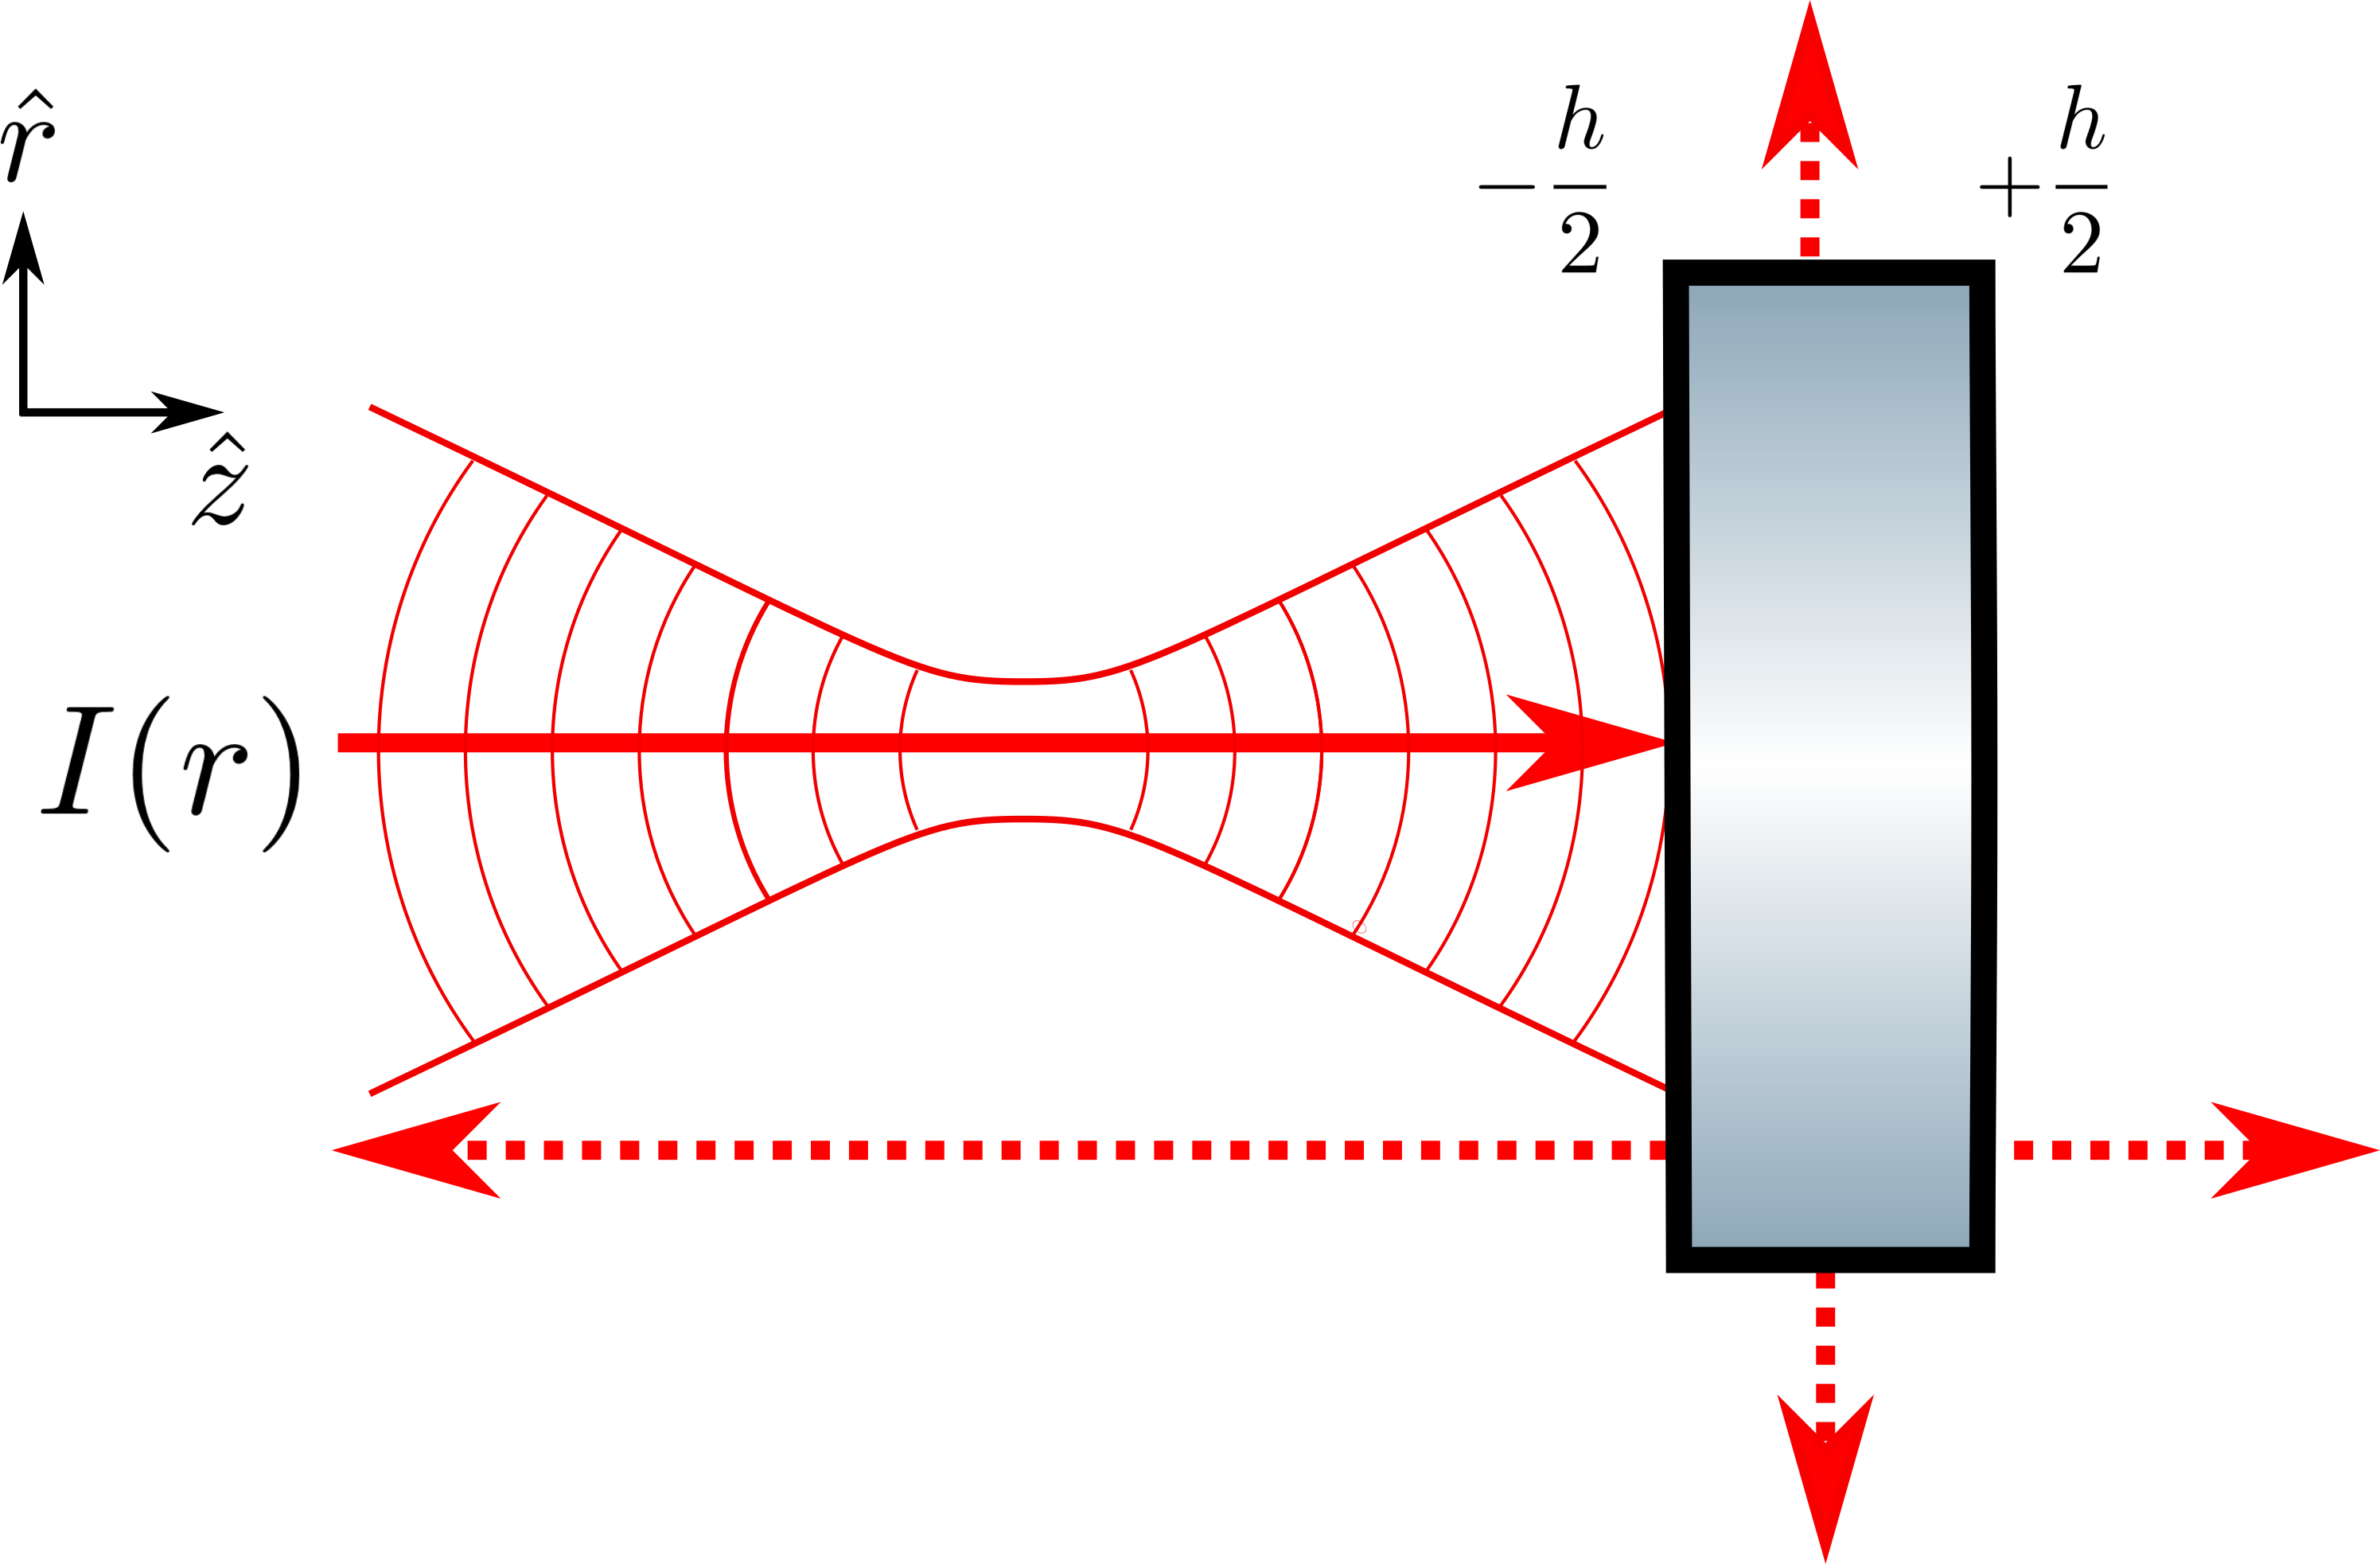
\includegraphics[width=.6 \textwidth]{../Figures/ThermalLensFlux.png}
		\caption[A conceptual model of flux balance for a cylindrical object.]  
		{\textbf{A conceptual model of flux balance for a cylindrical object.} The red dotted lines represent the radiative fluxes escaping the optic while a Gaussian beam with intensity profile $I(r)$ is pumping energy in as denoted by the red solid line.}
		\label{fig:ThermalLensFlux}
	\end{figure}

	At the surface where $z=h/2$ the total flux is radiative,
	\begin{equation}\label{eq:faceh2}
	-\kappa \frac{\partial T_p(r,h/2)}{\partial z} = 4 \sigma_B T_0^3 T_p(r,h/s)
	\end{equation}
	
	At the barrel of the cylinder where $r=a$, total flux is also radiative,
	\begin{equation}\label{eq:barrel}
	-\kappa \frac{\partial T_p(a,z)}{\partial r} = 4 \sigma_B  T_0^3 T_p(a,z)
	\end{equation}
	
	At the surface where $z=-h/2$ there are two components of flux, one is radiative and the second is the input power from the laser beam striking the optic surface,
	\begin{equation}\label{eq:face-h2}
		-\kappa \frac{\partial T_p(r,-h/2)}{\partial z} =  -4 \sigma_B T_0^3 T_p(r,-h/s) + \epsilon_a I(r)
	\end{equation}
	where $I(r) = \frac{2P}{\pi w^2} \exp{-2r^2/w^2}$ is the laser beam intensity with power $P$ over a beam size of $w$ and $\epsilon_a$ is the absorption coefficient.  Here, the radiative term has a negative sign to represent the flux direction. Once boundary conditions are established,  most introductory textbooks that deal with partial differential equations will apply an educated guess for the solution.  In this case, the resulting temperature field will be a harmonic function,
	\begin{equation}
	T_p(r,\phi,z) =  (A e^{+k z} + B e^{-kz}) J_0(kr)
	\end{equation}
	where $J_0$ is the spherical Bessel function of the first kind and $k$ is a constant.  Although this particular temperature distribution can be even more general by allowing all the orders of $J_n$, this form is sufficient. Using the boundary condition from \ref{eq:barrel} and the property $\frac{\partial J_0(x)}{\partial x} = -J_1(x)$,
	\begin{equation}
		-\kappa k \frac{\partial J_0(kr)}{\partial r} \bigg\vert_{r=a} = 4 \sigma_B T_0^3 J_0(ka)
	\end{equation}
	\begin{equation}\label{eq:sphere_bessel}
		ka J_1(ka) - \chi J_0(ka)=0
	\end{equation}
	where $\chi = 4\sigma T_0^3 a/\kappa$ is the reduced time constant.  There exists an infinite number of discrete solutions which can solve \ref{eq:sphere_bessel} using various values of $k_n a = \rho_n$.
	The temperature field then becomes,
	\begin{equation}\label{eq:temp2}
	T_p(r,z) = \sum_{n=0}^{\infty} (A_n e^{+k_n z} + B_n e^{-k_n z}) J_0(k_n r)
	\end{equation}
	In order to solve the conditions from equations \ref{eq:faceh2} and \ref{eq:face-h2}, the strategy is use the orthogonality of the spherical Bessel functions in order to expand the equations into a solvable algebraic form.  This will include expanding the intensity profile $I(r)$ in this basis as well.  Consider the boundary from $r=0$ to $r=a$, the functions $J_0(k_n r)$ form a complete basis set and the normalization constant is given by the Sturm-Louisville problem,
	\begin{equation}
	\int_{0}^{a} J_0(k_n r) J_0(k_m r) \,r \, \text{d}r= \delta_{mn} \frac{[\chi^2 + (k_na)^2]}{2k_n^2} J^2_0(k_na) = \delta_{mn} \frac{1}{N_n}
	\end{equation}
	Then expanding the intensity profile in terms of the Bessel function: $I(r)= \sum_{n}^{\infty} p_n J_0(k_n r)$ and inverting to solve for $p_n$ leads to,
	\begin{equation}
	\begin{aligned}\label{eq:p_n_gauss}
	p_n &= N_n \int_{0}^{a} I(r) J_0(k_n a) \, r \, \text{d}r\\
		&= N_n \int_{0}^{a} \bigg[\frac{2 P}{\pi w^2}\bigg] J_0(k_n a) \exp{-2r^2/w^2} \, r \, \text{d}r\\
		&\approx N_n \, \frac{P}{2\pi a^2} \, \exp{-\frac{(k_n w )^2}{8} } 
	\end{aligned}
	\end{equation}
	The approximation came from integrating to infinity instead of $a$ which is reasonable if diffraction losses are small on the substrate.  Plugging in the equation \ref{eq:temp2} and $I(r)$ into the remaining boundary conditions,
	\begin{subequations}
		\begin{equation}
		\bigg[ k_n - \frac{4\sigma_B T_0^3}{\kappa}\bigg] e^{-k_nh} A _n - \bigg[ k_n + \frac{4\sigma_B T_0^3}{\kappa}\bigg] B_n = \frac{\epsilon p_n  }{\kappa} e^{-k_nh/2}
		\end{equation}
		\begin{equation}
		\bigg[ k_n + \frac{4\sigma_B T_0^3}{\kappa} \bigg] A _n - \bigg[ k_n - \frac{4\sigma_B T_0^3}{\kappa}\bigg] B_n e^{-k_nh} = 0
		\end{equation}
	\end{subequations}
	Solving for $A_n$ and $B_n$,
	\begin{subequations}
		\begin{equation}
			A_n = \frac{\epsilon_a p_n}{\kappa} e^{-3k_n h /2} \frac{\eta_{+}}{\eta_{+} - \eta_{-} e^{-2k_n h} }
		\end{equation}
		\begin{equation}
			B_n = \frac{\epsilon_a p_n}{\kappa} e^{-k_n h /2} \frac{\eta_{-}}{\eta_{+} - \eta_{-} e^{-2k_n h} }
		\end{equation}
	\end{subequations}
	where $\eta_{\pm} = k_n \pm \frac{4\sigma_B T_0^3}{\kappa}$ is used for brevity. Now it is possible to write down the entire steady-state temperature field for a cylindrical test mass with a laser beam impinging on the surface,
	\begin{equation}
	T_p(r,z) = \sum_{n=0}^{\infty} \frac{\epsilon_a p_n}{\kappa}  \; \frac{ \eta_{-}e^{-k_n(3h/2-z)} + \eta_{+}e^{-k_n(h/2-z)}  }{\eta_{+} - \eta_{-} e^{-2k_n h} } J_0(k_n r)
	\end{equation} 
	Once the temperature profile is solved, the path length distortion from the thermo-refractive effect can be found by solving by equation \ref{eq:thermoref},
	\begin{equation}
	Z_{\text{TR}}(r) = \frac{\text{d}n}{\text{d}t} \frac{\epsilon_a}{\kappa} \sum_{n=0}^{\infty} \, \frac{p_n}{k_n} \, \frac{1- e^{-k_n h}}{[\eta_{+} - \eta_{-} e^{-k_nh}]} \; J_0(k_n r) 
	\end{equation}
	where $p_n$ contains information about the heating profile so it is possible to directly plug in equation \ref{eq:p_n_gauss} to represent the distortion from a Gaussian beam,
	\begin{equation}
	Z_{\text{TR}}^{G}(r) =  \frac{\text{d}n}{\text{d}t} \frac{\epsilon_a \, P}{2\pi a^2 \kappa} \sum_{n=0}^{\infty} \, \frac{N_n}{k_n}\, e^{-(k_n w)^2/8} \, \frac{1- e^{-k_n h}}{[\eta_{+} - \eta_{-} e^{-k_nh}]} \; J_0(k_n r) 
	\end{equation}
	The thermo-refractive effect due to coating and substrate absorption is only one type, there is also an effect which elastically curves the surface from thermal expansion \cite{Vinet_Thermal_Issues}.  This thermo-elastic effect deals with the internal stresses of the material and employs the stress-strain relations in order to derive the wavefront curvature.  For the LIGO test masses which use fused silica, this effect is smaller than the thermo-refractive wavefront distortion by about an order of magnitude.
	
	\section{Contrast Defect}
	Generally, the contrast defect is defined as the ratio of power between the antisymmetric port and the reflected port when locked on a dark fringe.  In other words, it is the amount of junk light that is present in the interferometer when light between the two arms do not perfectly interfere with each other. This junk light can be the symptom of various causes, for example, an imbalance of reflectivity between ITMX and ITMY will cause non-perfect destructive interference at the antisymmetric port and a camera would see a TEM00 beam when locked on length.  Another cause of contrast defect could be from misalignment between the ITMs or beamsplitter which will result in seeing a TEM 01/10 mode.  However, if both of the aforementioned causes are fixed with a combination of stringent design specifications for the reflectivity and alignment loops closed to minimize angular jitter, then the contrast defect will be dominated by mode mismatch which can be fixed by a combination of ring heaters and CO2 lasers.  The picture gets even more complicated when adding in the absorption for individual optics and introducing multiple Fabry-Perot cavities which will treat the sidebands and carrier fields differently.  One of the main goals for the Thermal Compensation System is to correct the cold and hot interferometer differences in radii of curvature.
	
	\subsection{Simple Michelson Contrast Defect}
	The simple Michelson can give a first estimate of the contrast defect when starting to commission the interferometer's thermal system, however, it is not used in nominal low noise since the dual-recycled Michelson is implemented.  By propagating the input mode cleaner beam to the beamsplitter and taking a single bounce at the high reflectivity surface, one can approximate the resultant mode overlap by measuring the power at the antisymmetric port.  The static mismatch correction was measured this way and is compensated using one of the CO2 lasers to reduce the contrast at 2 Watts of input power from $0.4\%$ to $0.1\%$.
	
	At this point the carrier and sideband fields follow the same ABCD matrix transfer function, so only one calculation is needed to estimate the contrast defect.  A keen reader will notice that this model will not take the Schnupp asymmetry into account which allows the $\hat{x}$-direction beam to travel an extra 8 centimeters further than the $\hat{y}$, however, this effect will only change the end result by approximately 10$\%$.  In fact, for this interferometer configuration, the dominate source of mismatch will be from the prompt reflection off the HR surfaces of the ITMs where most of the phase change occurs.  The sideband contribution at the antisymmetric port can be estimated by using equation \ref{sb_tf} and measuring the modulation depth, $\Gamma_{\Omega}$, for the 9 and 45 MHz RF fields that enter the interferometer,
	\begin{equation}
	\begin{aligned}
	P_{\text{SB}}	&= 2 P_{\text{in}} \bigg( \frac{\Gamma}{2} \bigg)^2 t_{SB\pm} \\
	&= 2 P_{\text{in}} \bigg( \frac{\Gamma}{2} \bigg)^2 \sin^2(k_{\Omega} \Delta \ell)
	\end{aligned}
	\end{equation}
	Additionally, the beamsplitter RMS motion will also contribute extra power at the AS and can be estimated by calculating the coupling coefficient from the 00 to 01 HG mode,
	\begin{equation}
	P_{01} = 2 P_{\text{in}} \bigg( \frac{\pi \, \alpha \, w(z)}{\lambda}\bigg)^2
	\end{equation}
	where $w(z)$ is the beam size on the test mass and $\alpha$ is the misalignment RMS.
	
	\subsection{Modal Contrast Defect}
	During full lock, the formalism must be extended to include the mode shape of two arm cavities interfering at the beamsplitter. Using the Laguerre-Gauss modes is useful for brevity because the mode mismatch couples to only one higher order mode. Contrast defect can be defined using the zeroth eigenmode of each arm and then expanded to project the X-arm's basis onto Y-arm using higher order LG modes, $LG^{00}_y \rightarrow  LG^{00}_x + \alpha LG^{10}_x$.  Where $\alpha = \frac{1}{\sqrt{2}} \big(\frac{\Delta \omega_{0}}{\omega_{0}} + i \frac{\Delta z }{z_R}\big)$ is the amount of higher order mode coupling due to mismatch in beam size and location, respectively (see Chapter 3).
	\begin{equation}\label{CD_mode}
	\begin{aligned}
	\text{CD} 	&\equiv \frac{P_{AS}}{P_{REFL}} \\
	&= \frac{\vert LG^{00}_x - LG^{00}_y \vert^2}{\vert LG^{00}_x + LG^{00}_y \vert^2}\\
	&= \frac{\vert LG^{00}_x \vert^2 + \vert LG^{00}_x + \alpha LG^{10}_x \vert^2 - 2\Re(LG^{00}_x [LG^{00*}_x + \alpha LG^{10}_x ])}{\vert LG^{00}_x \vert^2 + \vert LG^{00}_x + \alpha LG^{10}_x \vert^2 + 2\Re(LG^{00}_x [LG^{00*}_x + \alpha LG^{10}_x ])}\\
	&\approx \frac{\alpha^2}{4}\\
	&\approx \frac{1}{8} \bigg[ \bigg(\frac{\Delta\omega_{0}}{\omega_{0}} \bigg)^2+  \bigg(\frac{ \Delta z }{z_R}\bigg)^2 \bigg]
	\end{aligned}
	\end{equation}
	Mismatch between the arm cavities can stem from a few sources such as the difference between the radii of curvature on the high reflectivity surfaces that will cause the resonant modes to be shaped differently between the X-arm and Y-arm. LIGO tries to optimize this effect by pairing the optics based on their properties, however, during the upgrades from O2 to O3 at Hanford, ITMX was replaced but ITMY was not which lead to a static mismatch between the input test masses.
	
	\section{Tuning Thermal Compensation for LIGO}
	
	As mentioned in Section \ref{Sec:TL_lensing}, the circulating power in each of the arms can be close to 150 kW for O3 and higher for the next observation runs.  Even with absorption estimates between $0.2-0.8$ parts per million, the induced substrate lensing can be significant.  The Thermal Compensation System (TCS) \cite{Lawrence_TCS} \cite{AWC_current} \cite{winkler_thermaldist} \cite{Strain_TL} was developed to correct the wavefront by applying heat to cancel the deformities caused by interferometer heating.  Lock acquisition and gravitational-wave optimization are the main metrics for success when commissioning most LIGO systems.  To aid in the former, TCS is required to thermally lens the substrate between the beamsplitter and high-reflectivity surfaces of the test masses such that the optical path difference is optimized for the carrier and sideband power recycling gains.  Both deal heavily with mode-matching the arm cavities such that overlap between the Gaussian modes is maximized.
	
	To optimize the TCS settings for the best power build-ups, there are two separate strategies:  The first requires estimating the amount of absorption on the test masses with the Hartmann Wavefront Sensors to measure the optical path distortion induced by the interferometer during a lock loss.  Then pre-load the ring heaters with the nominal settings which would cancel carrier beam's thermal absorption in the "hot" state.  The ring heaters have a very long time constant (30 hours) to reach thermal equilibrium with a step response of electrical power, so if there is compensation needed, the heaters must be energized at all times.    However, turning them on will change the radius of curvature and induce a substrate lens (see Section \ref{Sec:RH}) that has to be canceled out by the CO2 (Carbon Dioxide) lasers which create a lens on the compensation plate of the quadruple pendulum.  Since the CO2 lasers have a time constant of approximately 0.5 hours, they can be turned up during lock acquisition and reduced as needed when the interferometer input power is increased. The second method is to use relevant interferometer RF signals at various ports to experimentally adjust the lensing commonly or differentially to maintain power recycling build-ups while increasing the interferometer input power.  In principle, either method should lead to the same answer but in practice, both are used to find the nominal thermal compensation configuration.
	\subsection{Hartmann Wavefront Sensors}\label{Sec:HWS}
	All estimates of steady-state curvature changes due to heating by the main interferometer beam depend linearly on the absorption and this can be quite difficult to detect when the coating absorption are typically less than one part in a million.
	
	In order to diagnose this effect, the Hartmann Wavefront Sensors (HWS) \cite{Brooks_OffAxis} \cite{Veitch_HWS_ALIGO} was a system developed by Adelaide and Caltech \cite{Brooks_HWS_2007} \cite{Brooks_HWS_2009} which use an auxiliary beams and charged-coupled imaging devices (CCD) to sense the wavefront distortions formed by heating from the interferometer beam during power up and a lock loss.  Currently, there are four Hartmann sensors installed at each test mass, which are injected from the AR surface side of the optics. Technical constraints require the ITM HWSs optical paths to differ from the ETM HWSs but the concept is still the same, so for brevity, only the ITMs HWSs will be discussed in detail.  In Figure \ref{fig:HWS_optical}, the system starts with an auxiliary super-luminous LED (SLED) beam being injected into the vacuum system and a telescope (Lens 1, Lens 2) which collimates/expands the beam to sample a space 200 mm in diameter on the test mass HR surface.  The return beams are picked-off and sent to a CCD with a Hartmann plate mounted on the front which effectively decompose the wavefront into individual rays.  Using a wavefront from a previous time with a cold optic as a reference. The Hartmann code creates a gradient vector field between the two times which have information about thermal lensing. Then numerically integrates the gradients to fit a wavefront field which is normally referred to as the optical path distortion in length units.  The algorithm then uses the Zernike polynomials as a single basis to represent the effective thermal lens. \cite{Brooks_thesis}
	
	\begin{figure}[!]
		\centering
		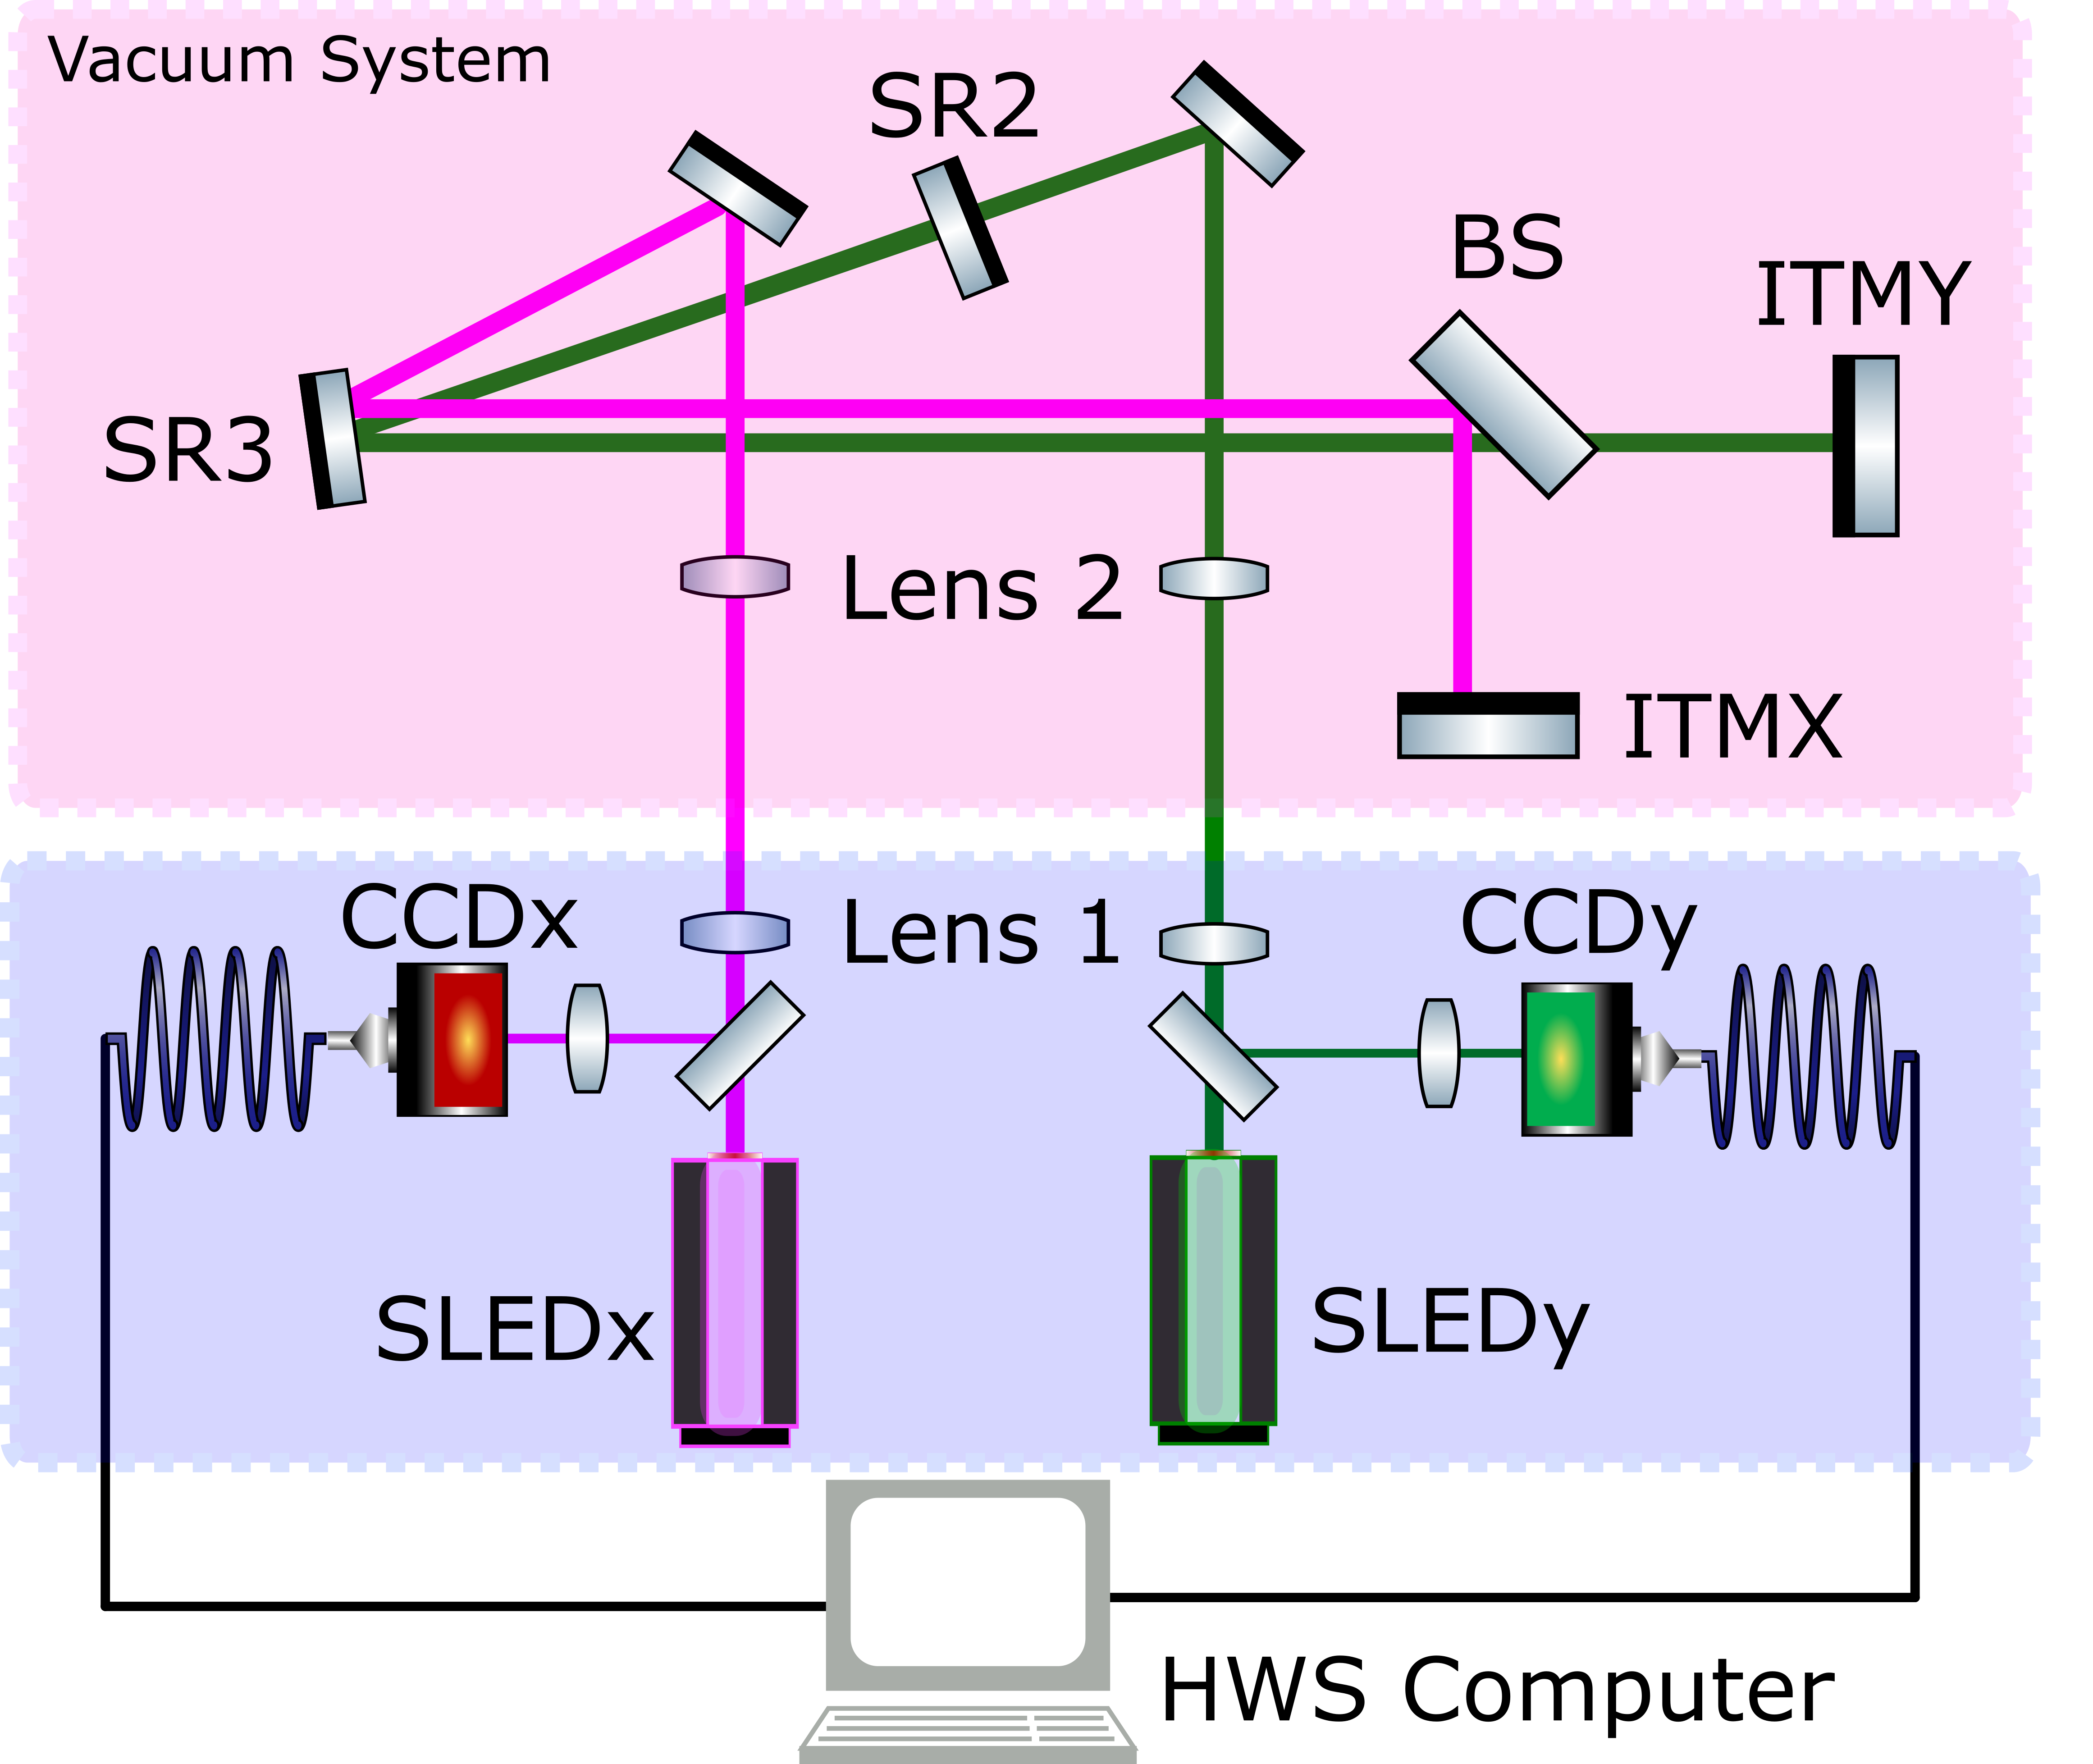
\includegraphics[width=0.6\textheight]{../Figures/HWS_OpticalLayout.png}
		\caption[ITM Hartmann sensors optical layout.] 
		{\textbf{ITM Hartmann sensors optical layout.} The path for injection is different for the two Hartmann sensors which use separate wavelengths to take advantage of the main beamsplitter AR/HR surface reflectivity. The ITMX (magenta) and ITMY (green) probe beam wavelengths are 800 nm and 833 nm, respectively, and have a 40 nm linewidth \cite{AWC_current}. The beams are sent into the vacuum system and retro-reflected off their respective optics back towards the pick-off mirrors before going into the CCDs with a Hartmann plate attached.  The cameras are then sent via fiber to a computer that runs the analysis pipeline on the images and exports the data to EPICS so the users can interface with the real time digital system in the control rooms.}
		\label{fig:HWS_optical}
	\end{figure}

	\begin{figure}[!]
	\centering
	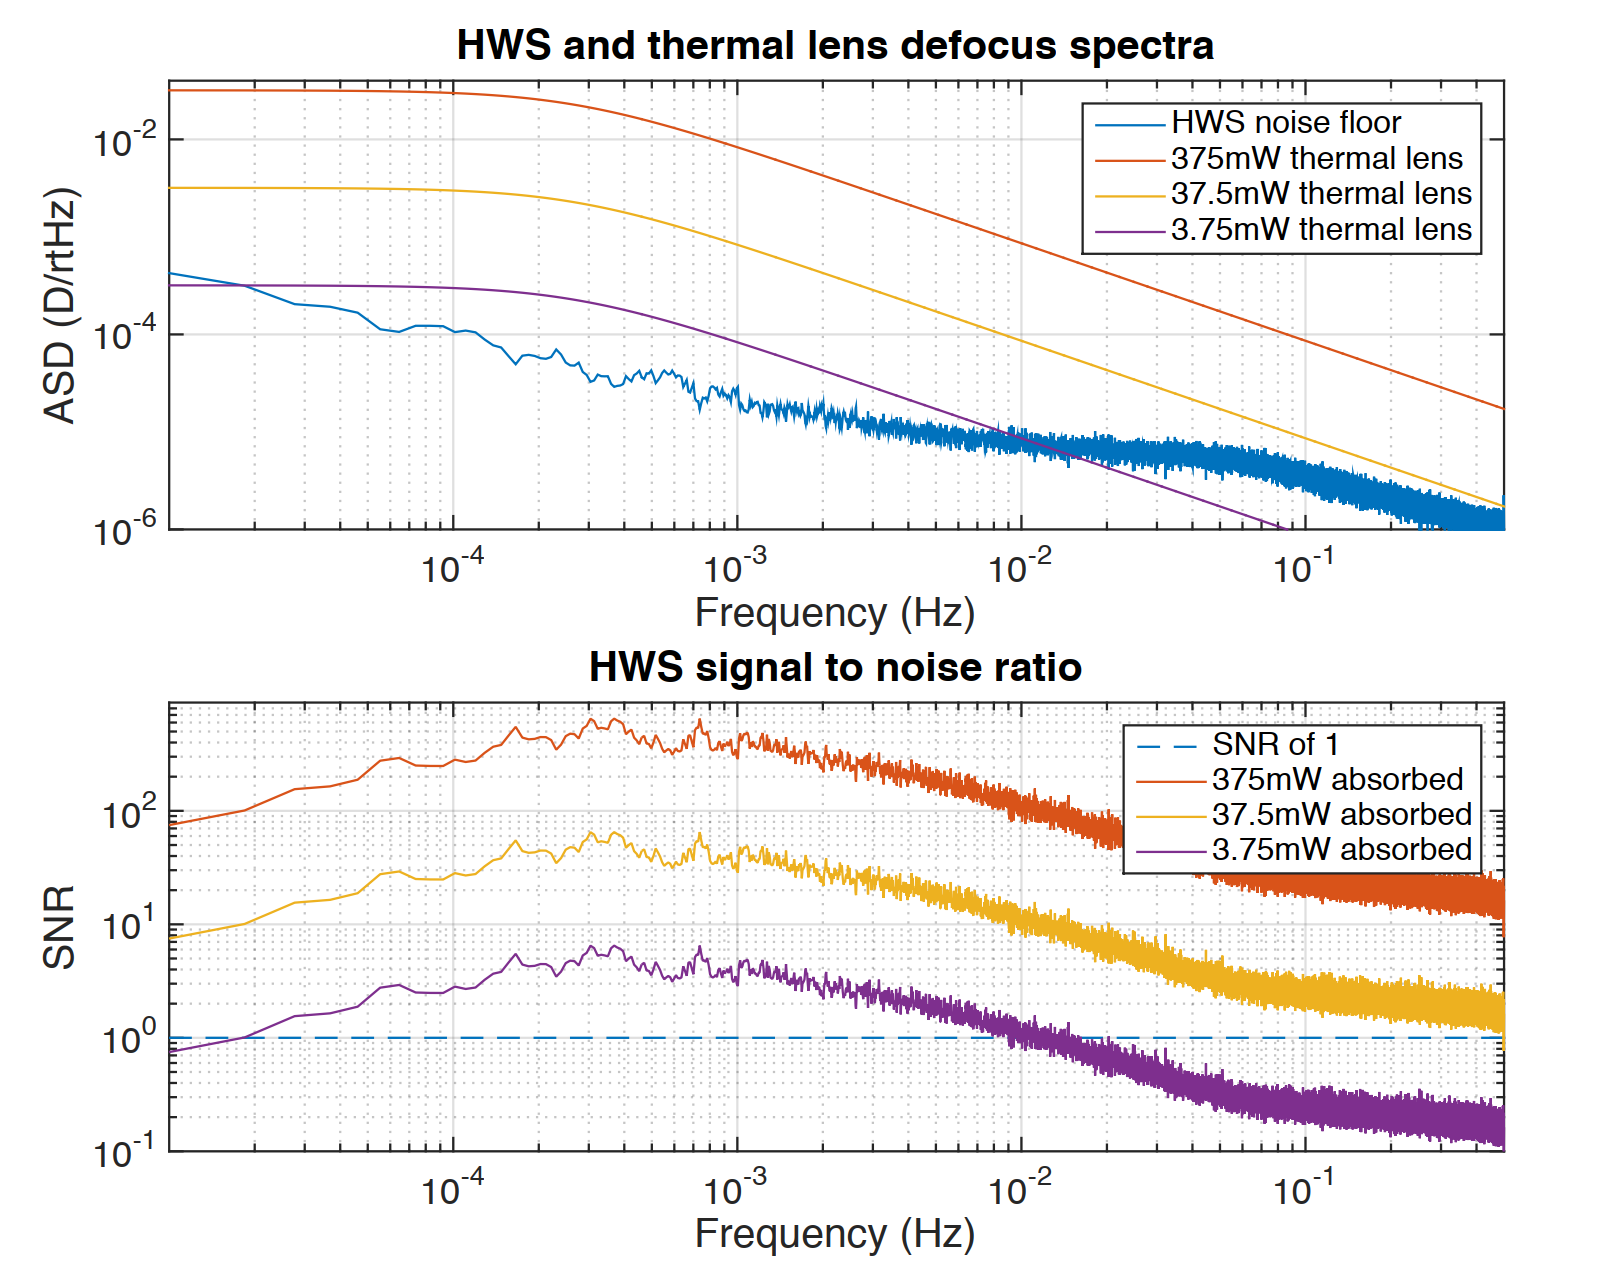
\includegraphics[width=0.7\textheight]{../Figures/HWS_Noise.PNG}
	\caption[Noise spectra for the HWS spherical lensing.] 
	{\textbf{Noise spectra for the HWS spherical lensing.} Taken from \cite{AWC_current}, this puts a lower bound on the Hartmann sensitivity to distortions for various time scales.}
	\label{fig:HWS_spectra}
	\end{figure}
	
	\subsubsection{Tuning the Hartmann Sensors}
	A source of systematic noise was from beam clipping in chamber on the ITMX HWS, see Figure \ref{fig:ITMX_clipping}. This creates fringes which are extremely sensitive to misalignment; one bandage that was applied to reduce this noise was to digitally mask the fringes so they do not confuse the fitting algorithms.  Hand tuning must be done so the mask is wide enough and centered around the interferometer lensing but not so large that the Hartmann fitting is corrupted by the fringes.  The aperture is very tight from baffles and are relatively far field from the CCD plane.  Two in-air periscope mirrors with pico-motors were used for alignment but beam clipping could not be fully removed.  This artifact was also found at LLO so it suggests a systematic error in the alignment scheme.  A possible fix could be implemented by replacing an in-vacuum steering mirror with a pico-motor.
	
	\begin{figure}[!]
		\centering
		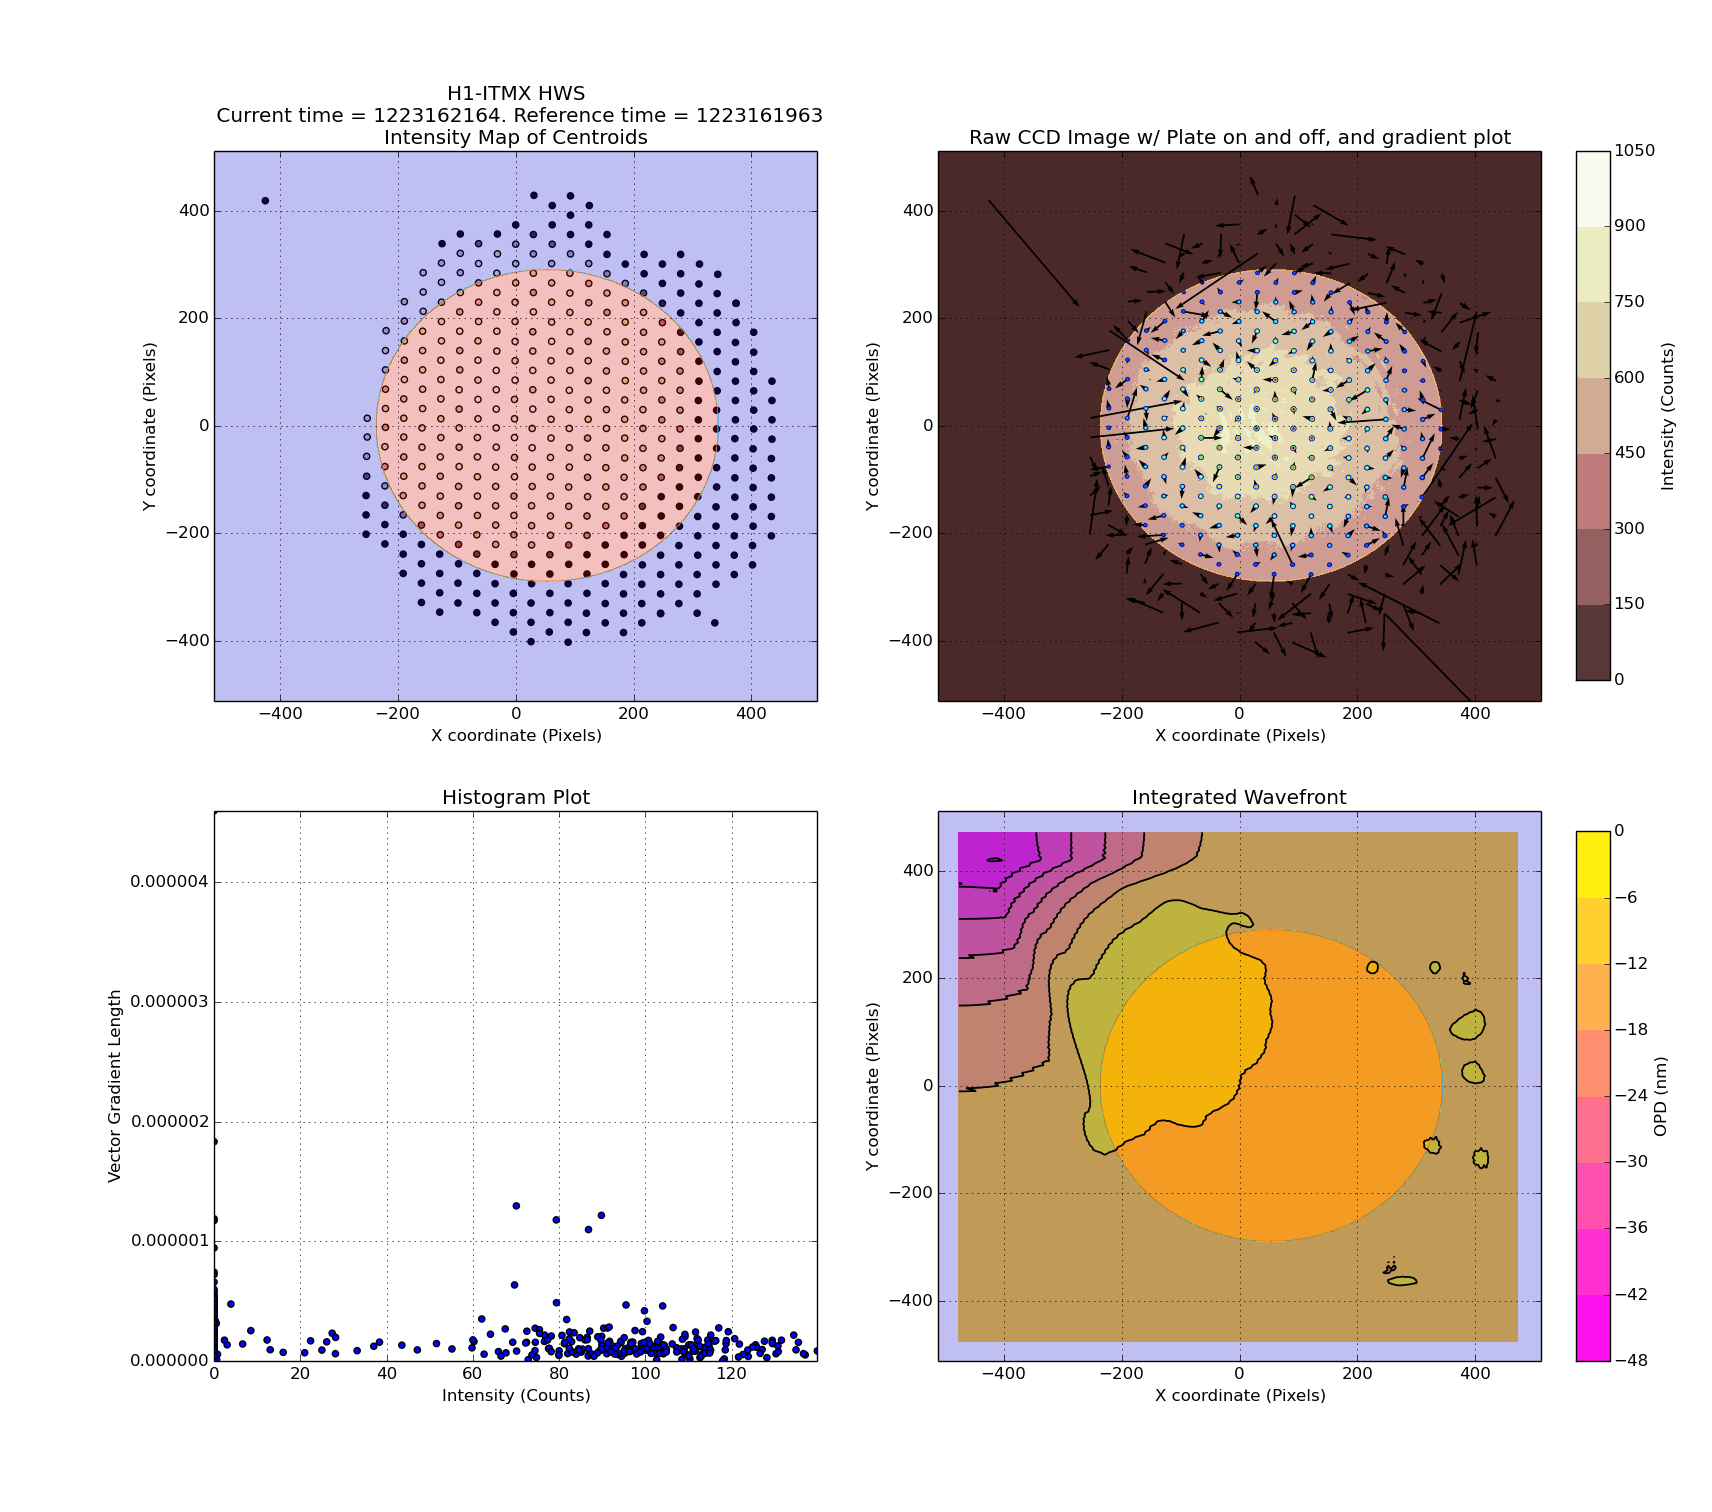
\includegraphics[width=0.7\textheight]{../Figures/20181011_ITMX_HWS_histogram_Masked.png}
		\caption[ITMX Hartmann Sensor output.] 
		{\textbf{ITMX Hartmann Sensor output.} Between the reference and current times for this measurement, no heating was applied to the test masses so the expectation is a relatively flat and smooth wavefront. This is mostly true except for a large, anomalous arrow at pixel coordinate [X,Y] = [-410, 405] of the gradient plots (upper right) which leads to a false wavefront distortion in the same area for the contour plot (lower right).  The sharp iris in the middle represents a digital mask that is can be turned on to reduce the effects of fringing.  A histogram in the bottom left plot shows the intensity distribution for each of the gradients; if the HWS beams are co-aligned well with the interferometer beam, then most of the information about thermal lensing occurs near the center of the intensity distribution.}
		\label{fig:HWS_Histogram}
	\end{figure}

	It was also found that the CCDs (Dalsa pantera 1m60) had a number of pixels which would create large spikes in their intensity counts and produce large artifacts in the gradient plots that corrupted the spherical lens fitting (see Figure \ref{fig:HWS_Histogram}).  One of the requirements for the HWSs is a wavefront distortion resolution of 1.35 nm \cite{AWC_current} and a single glitch could register a few orders of magnitude higher.  A solution for this was implemented by using the dark images to locate the bad pixels by averaging the counts over a few minutes and finding all the pixels which have counts higher than a particular threshold, generally 1.5 times above the average ambient dark noise level (about 50 counts).  The dark frames would be read in by the Hartmann code which has a module written by Adelaide that uses the dark images as references to find the average of surrounding pixels and replace the problematic pixel.  This digital procedure greatly reduced the amount glitches found in the Hartmann sensor data.
	
	\begin{figure}[t!]
		\centering
		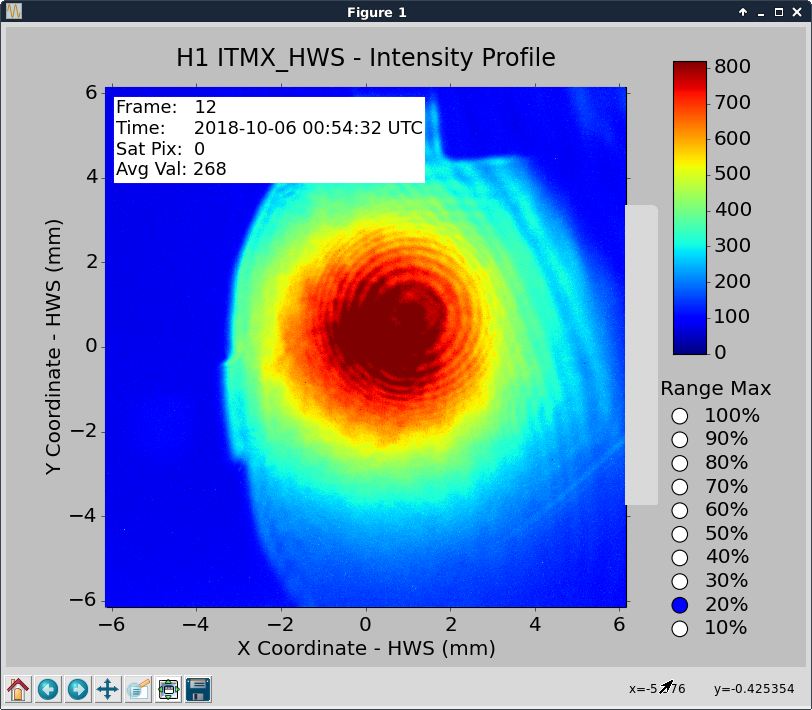
\includegraphics[width=0.4\textheight]{../Figures/ITMX_HWS_clipping.png}
		\caption[Clipping on ITMX Hartmann Sensor.] 
		{\textbf{Clipping on ITMX Hartmann Sensor.}  A source of systematic noise found at both sites when trying to simultaneously align ITMX and ITMY Hartmann Sensors.  The CCD spot positions are very sensitive to the SR3 alignment so control loops and initial alignment are not recommended for this particular optic.  An in-vacuum pico-motor may help alleviate the clipping.
		}
		\label{fig:ITMX_clipping}
	\end{figure}
	
	When increasing the input power into the interferometer, there were large spikes associated with the spherical power estimation on the ITMX.  This was eventually tracked down to leakage beam introduced by stray light from the interferometer.  At times, the leakage beam was 40\% the intensity of the main Hartmann beam which severely distorted the fitting algorithms. ITMY HWS did not see this effect because SR2 is such a good high reflector and attenuated any 1064 nm contributions down to the PPM level.
	
	\begin{figure}[t!]
		\centering
		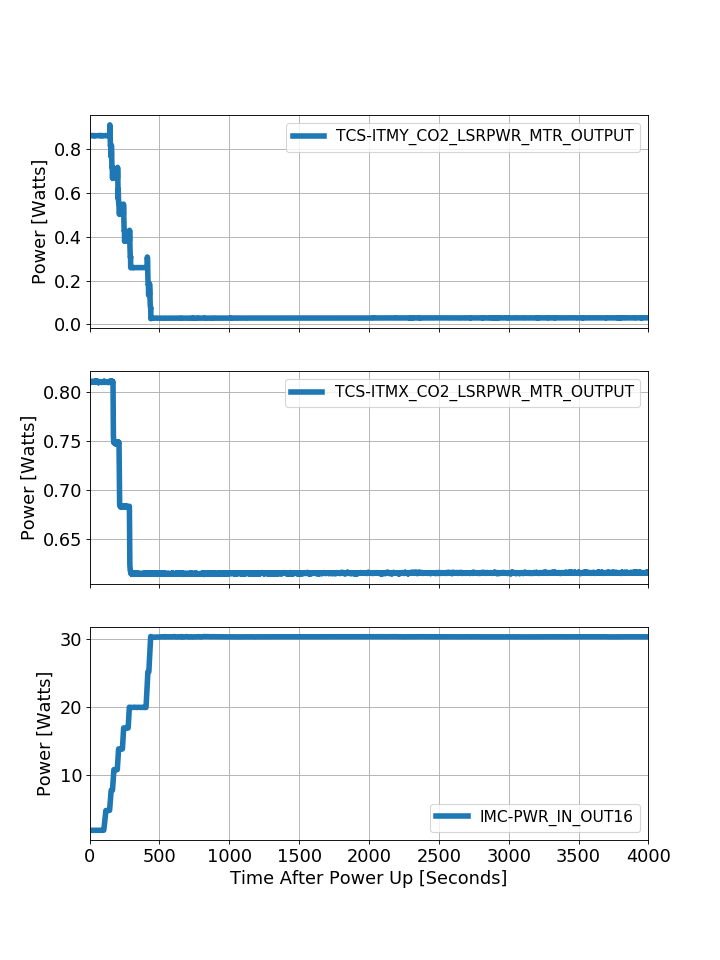
\includegraphics[width=0.45\textwidth]{../Figures/1231726400TCS_and_PSL_powerup.png}
		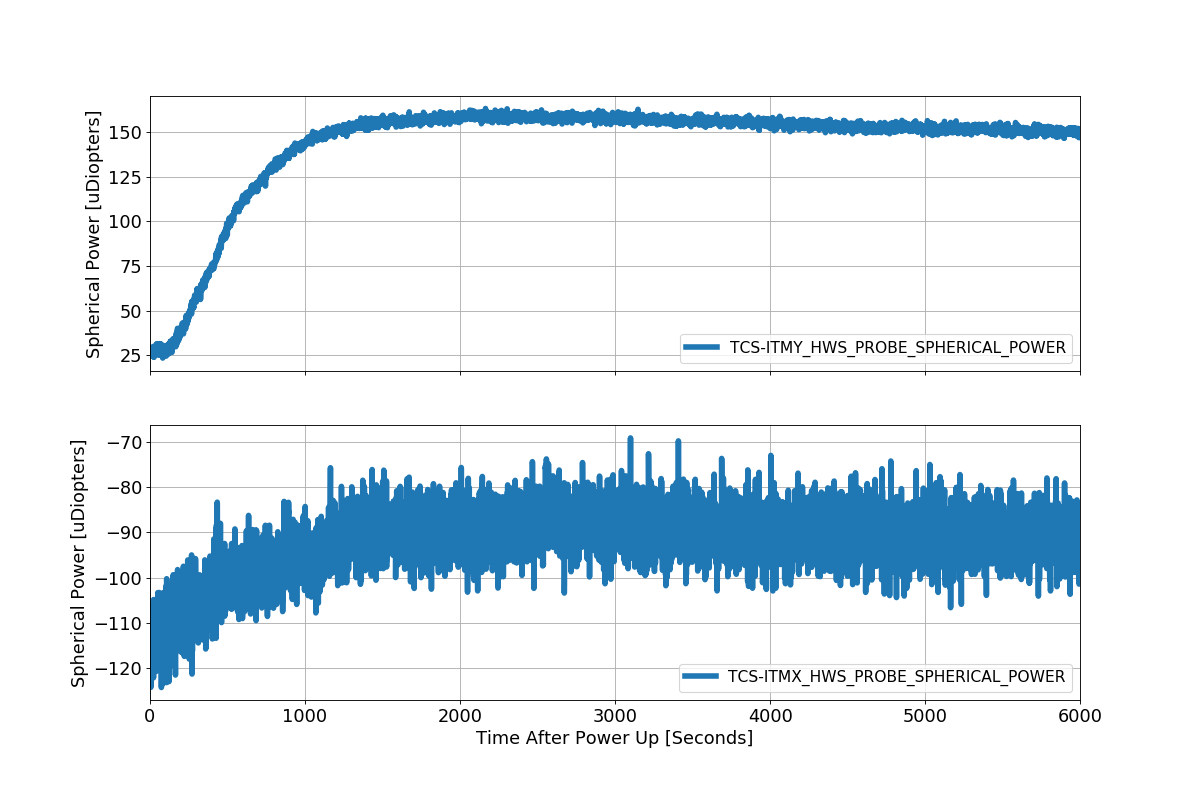
\includegraphics[width=0.45\textwidth]{../Figures/1231726400HWS_powerup.png}
		\caption[A time series of the interferometer power increase sequence.] 
		{\textbf{A time series of the interferometer power increase sequence.} 
			During this time, the interferometer is using DC-readout and locked at 2 watts of PSL input power with all of the angular control loops closed with high-bandwidth, in this configuration, the power recycling gain is approximately 45.  The left figure shows the increase of PSL input power and the CO2 lasers stepping down in power where levels of compensation were experimentally determined such that the angular control loops were stable and sideband build ups remained as high as possible.  The right plot shows the Hartmann sensor spherical power as a function of time with the starting point scaled to zero micro-diopters.  Although the point absorbers do not exhibit the same spatial structure as uniform heating so it is difficult to derive absolute absorption for ITMY, the spherical fitting gives some information about the relative scale of heating absorption between the two optics.}
		\label{fig:pwr_up_time}
	\end{figure}
	
	\begin{figure}[t!]
		\centering
		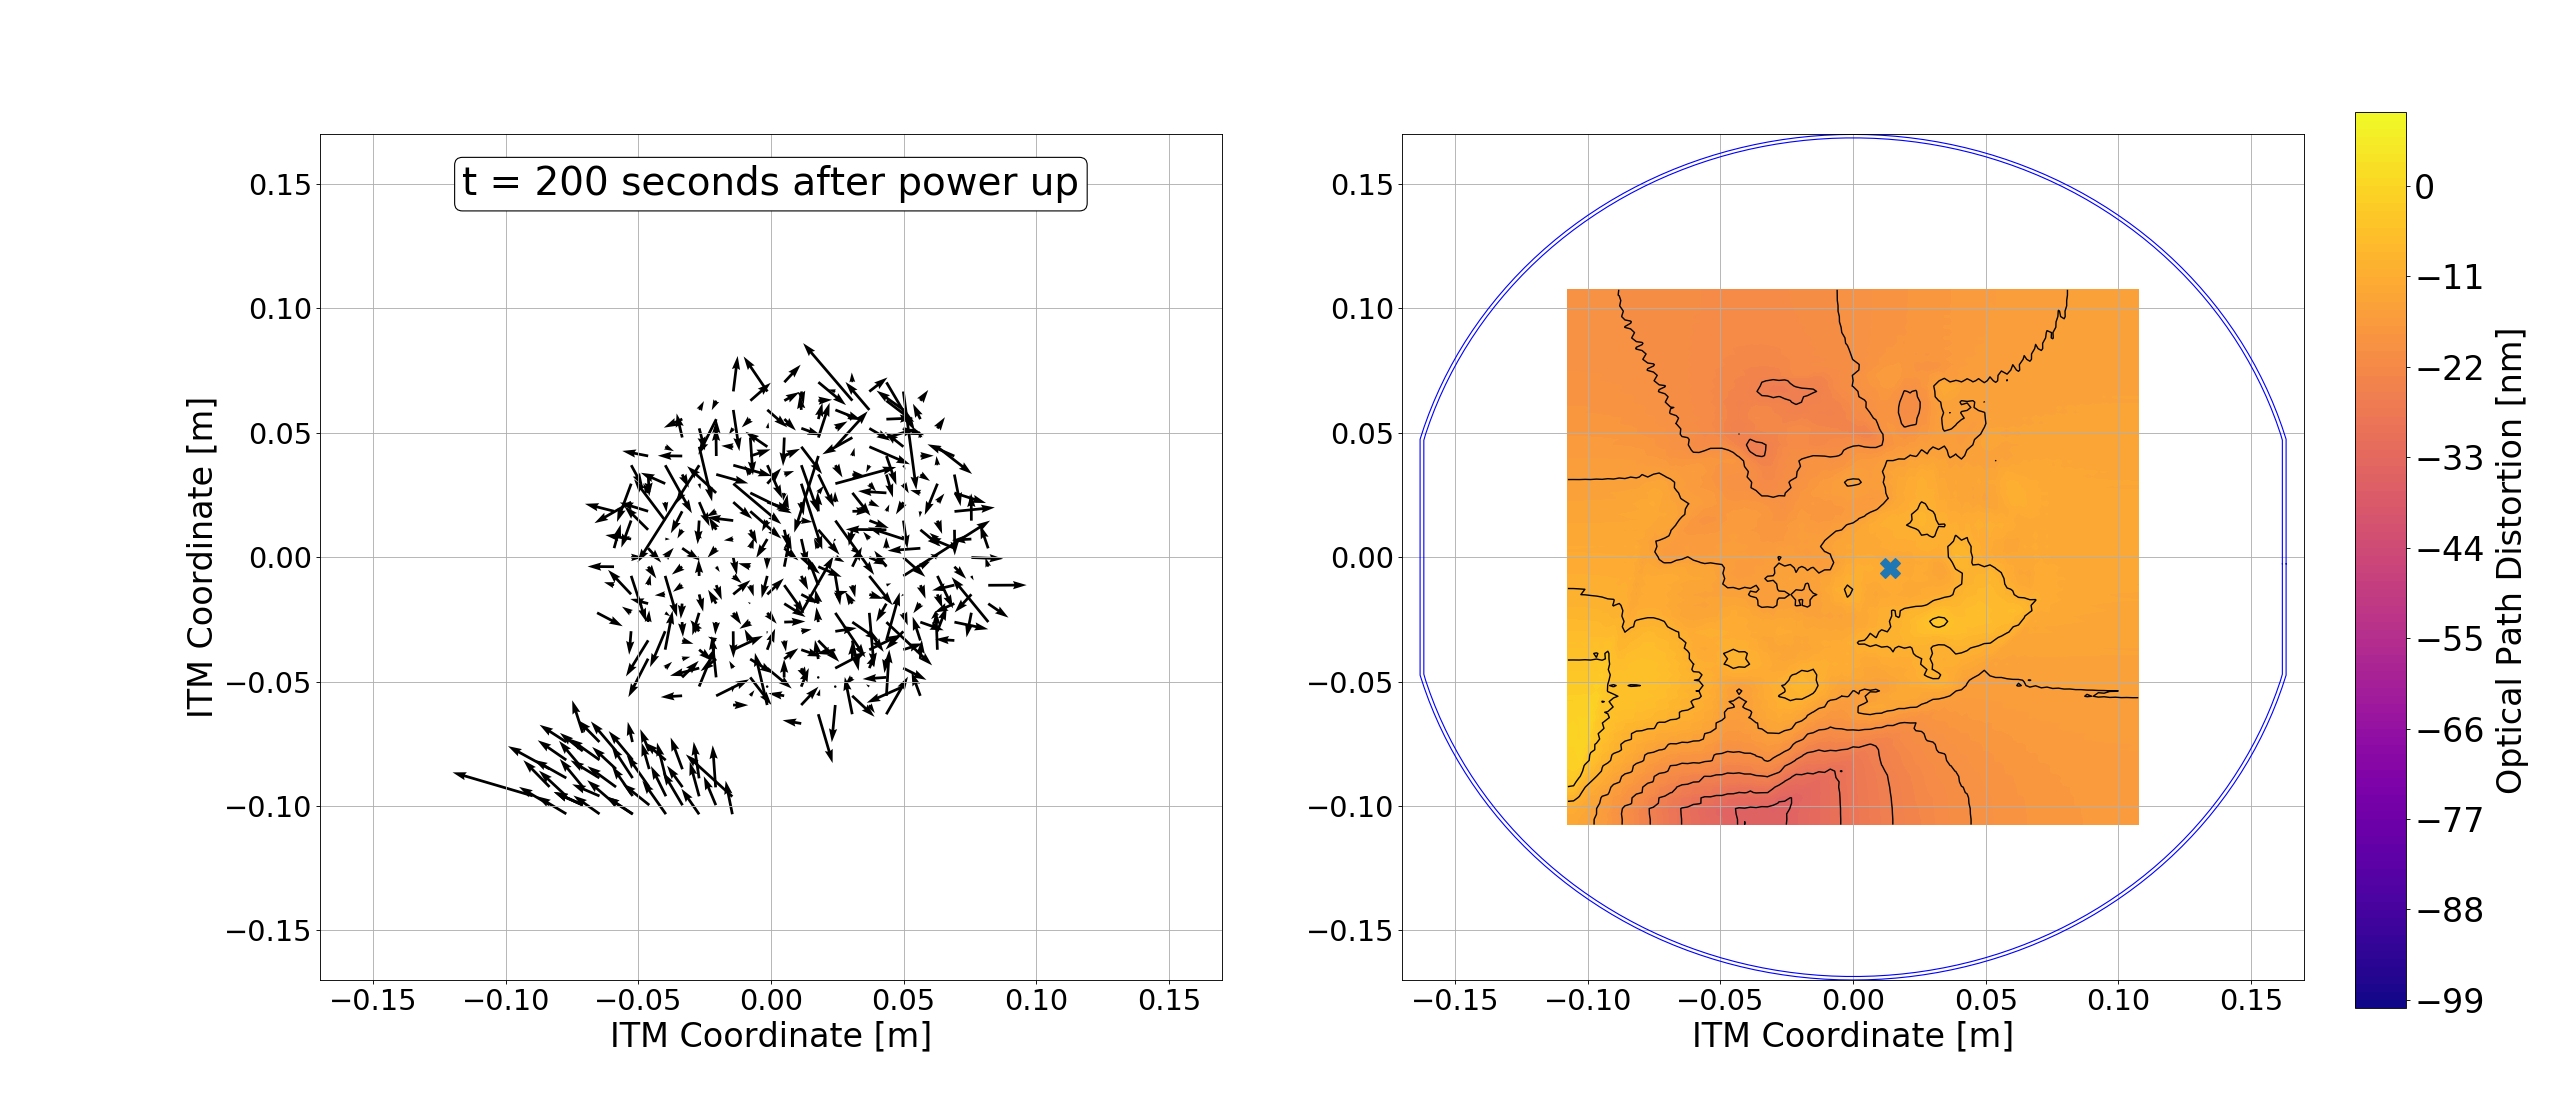
\includegraphics[width=0.55\textheight]{../Figures/1231726400_200dur_30W_ITMx.png}\quad
		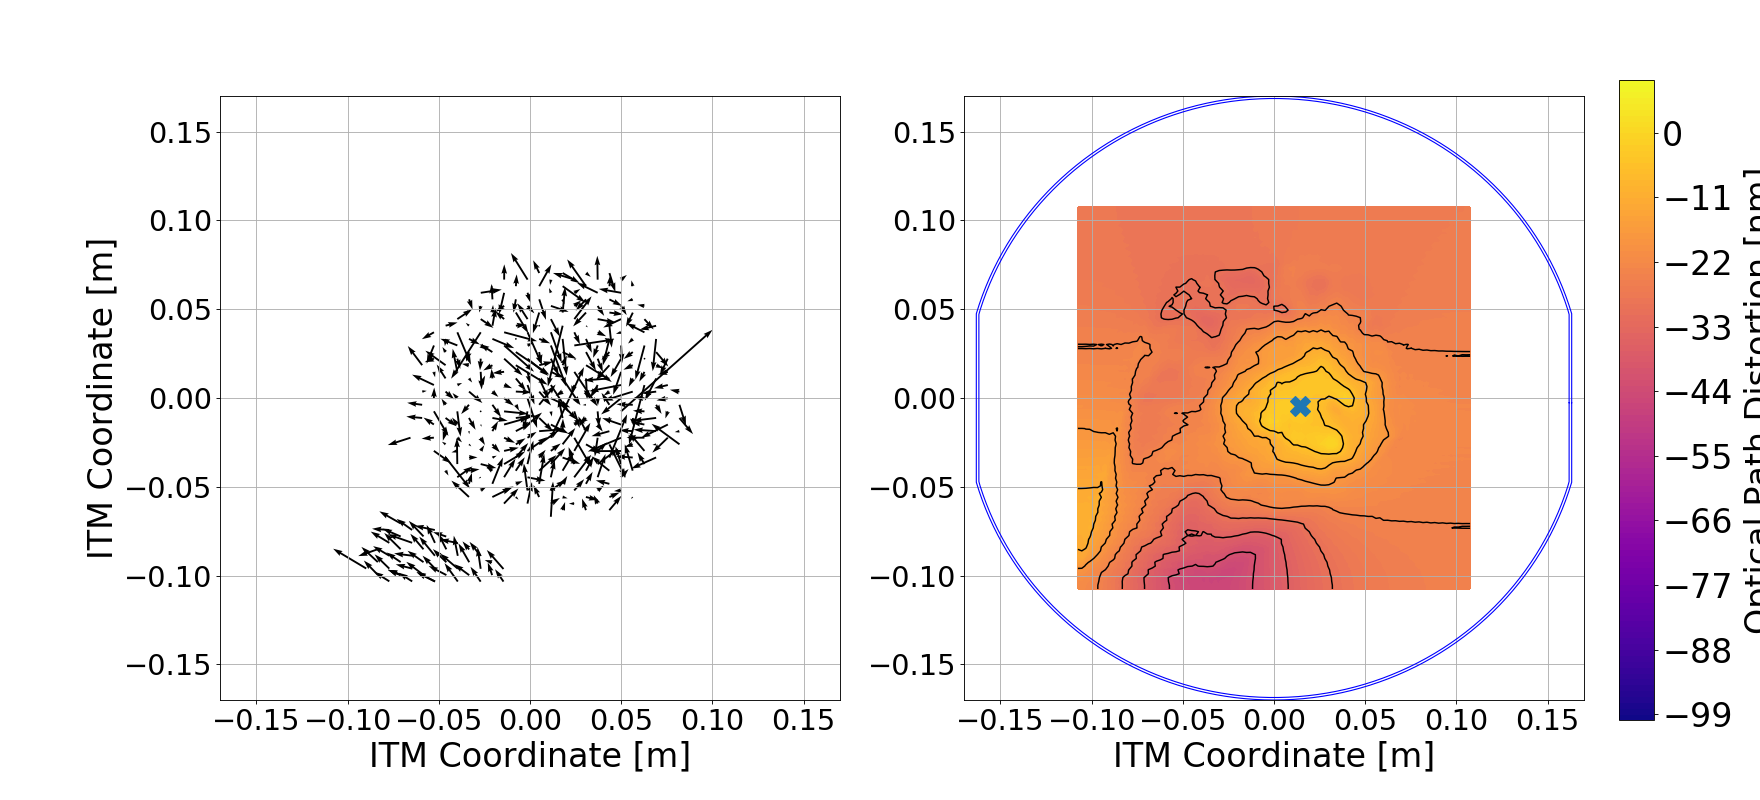
\includegraphics[width=0.55\textheight]{../Figures/1231726400_500dur_30W_ITMx.png}\quad
		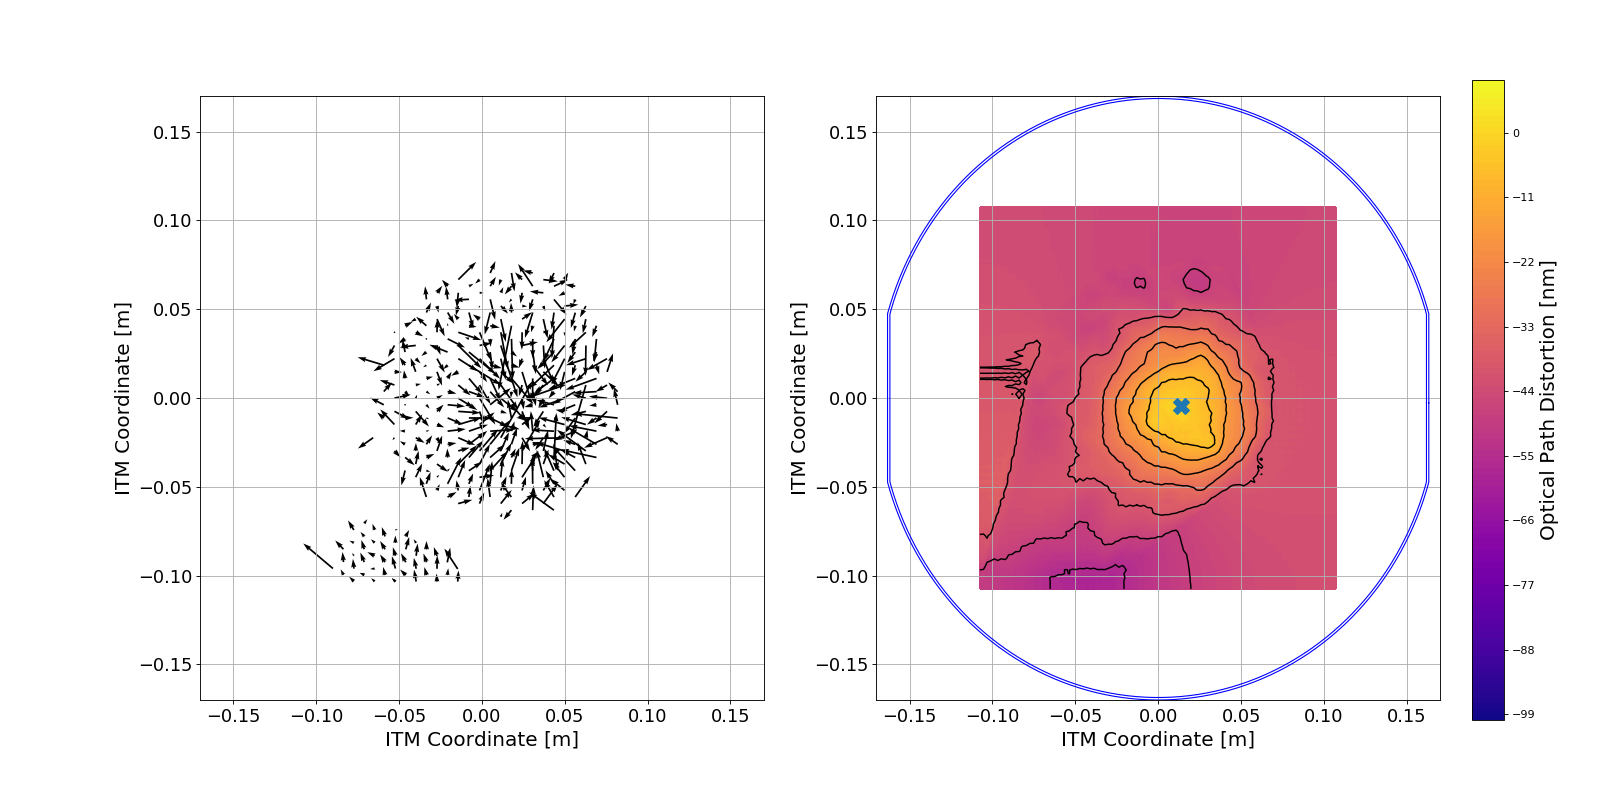
\includegraphics[width=0.55\textheight]{../Figures/1231726400_1000dur_30W_ITMx.png}\quad
		\caption[ITMX gradient plots (left) and wavefront maps (right) during a power up to 30 Watts of input power.]  
		{\textbf{ITMX gradient plots (left) and wavefront maps (right) during a power up to 30 Watts of input power.}
			It is important to note that there is a back-reflected stray beam from the super-luminous LED that is incident in the bottom left portion of the camera which is digitally cropped out during the real-time analysis. As previously noted, this particular Hartmann sensors suffers from beam clipping on the right side of the image which adds to the systematic noise.  A blue cross denotes the origin which is fitted with the Zernike polynomials to derive a spherical power.  The arrow lengths in the gradient plots are normalized to each individual plot and are meant to guide the eye in discerning the directionality and pattern of lensing.}
		\label{fig:ITMX_HWS_plot}
	\end{figure}
	
	\begin{figure}[t!]
		\centering
		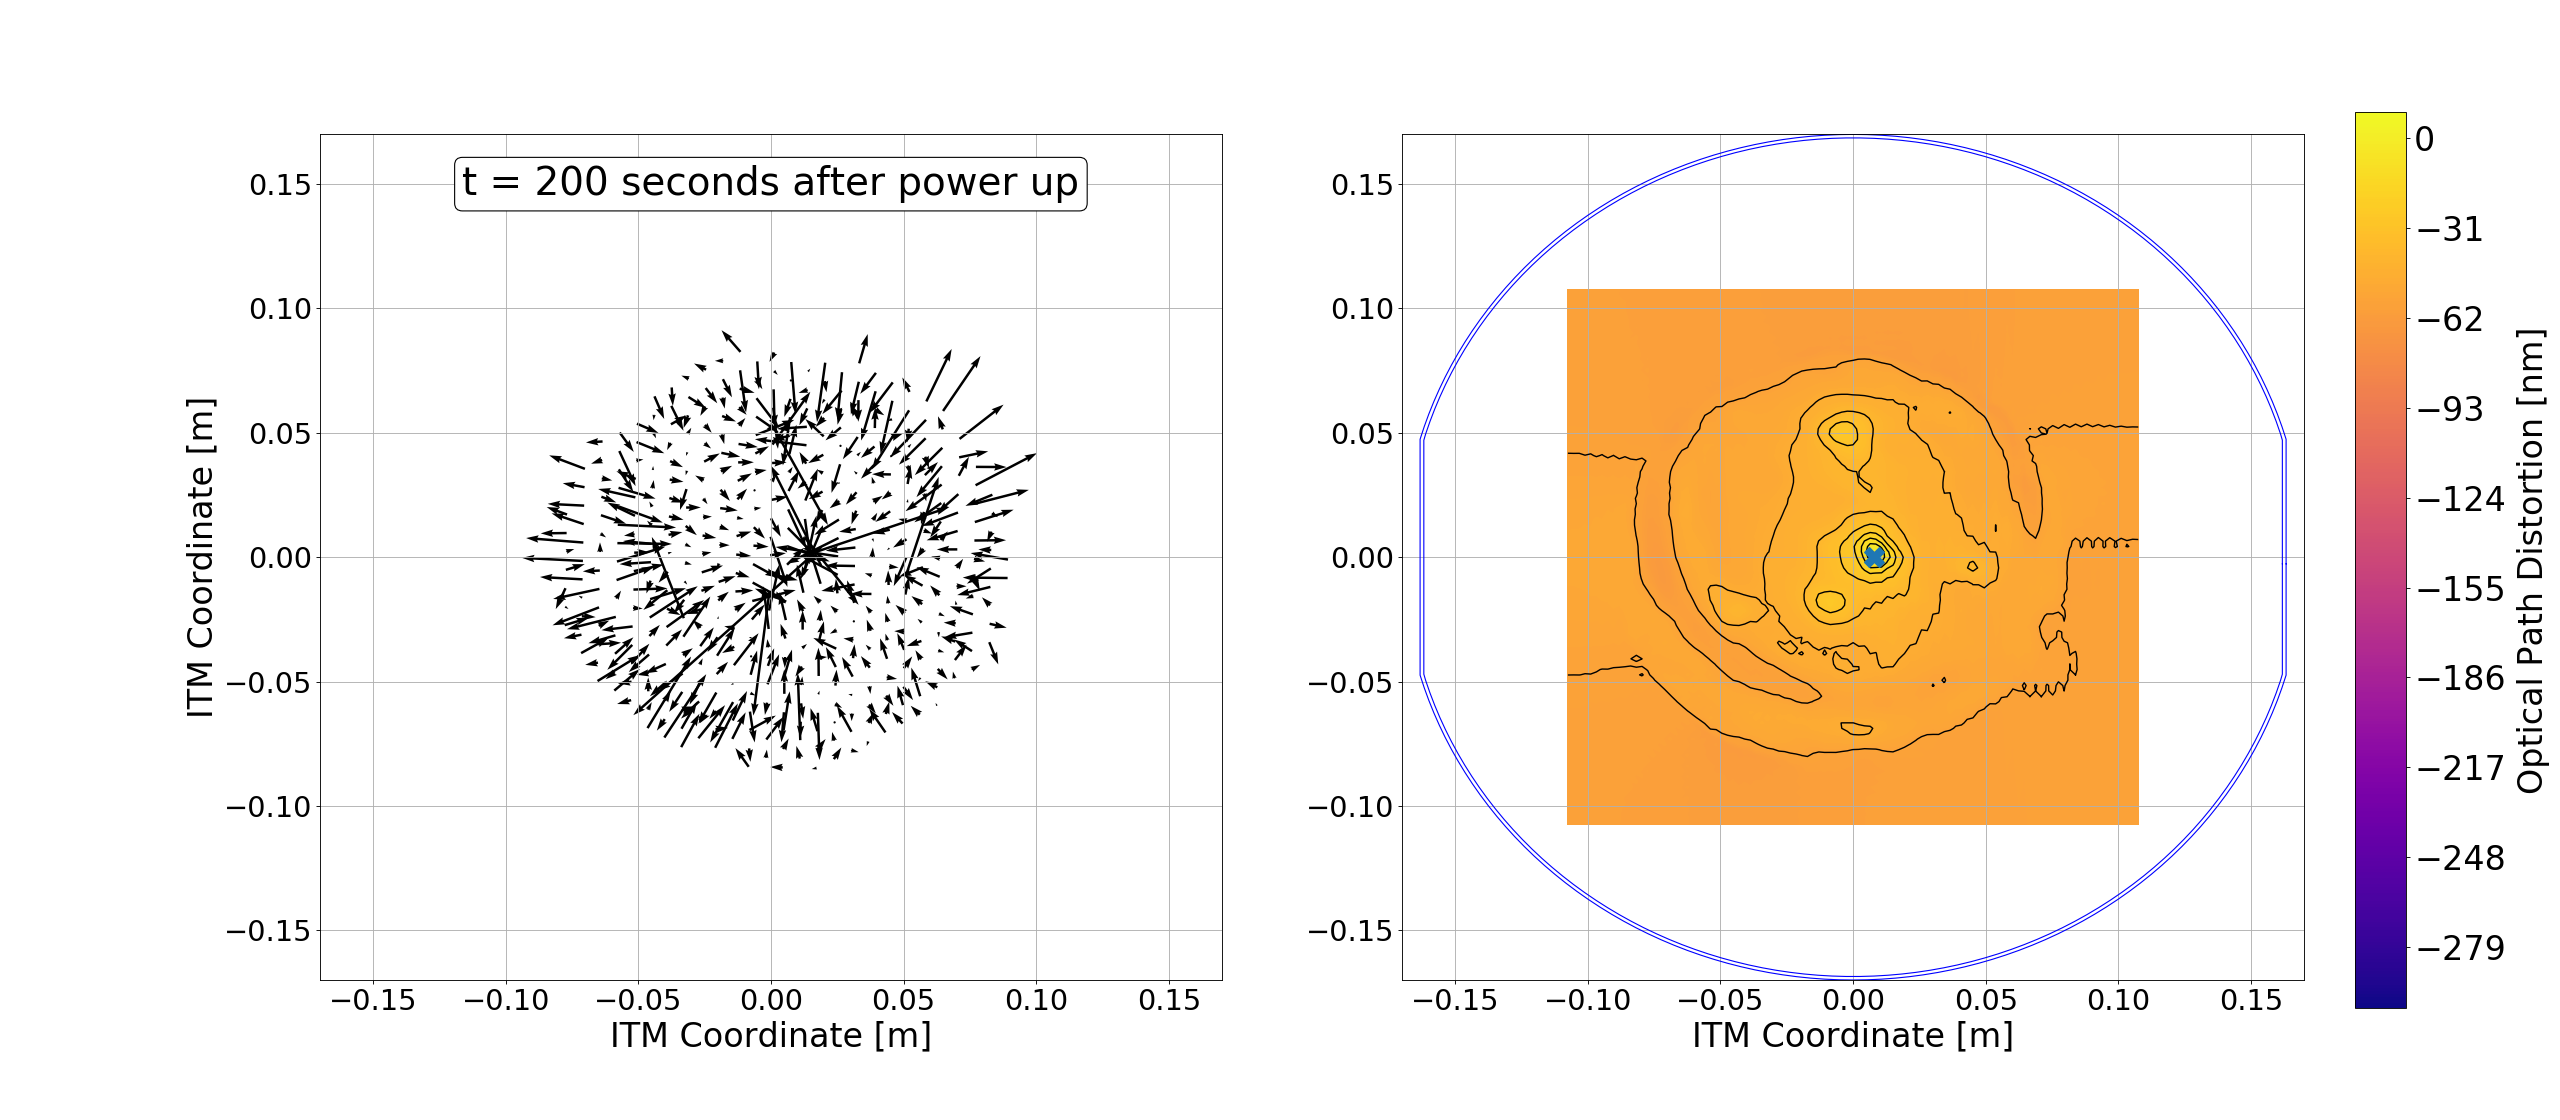
\includegraphics[width=0.55\textheight]{../Figures/1231726400_200dur_30W_ITMy.png}\quad
		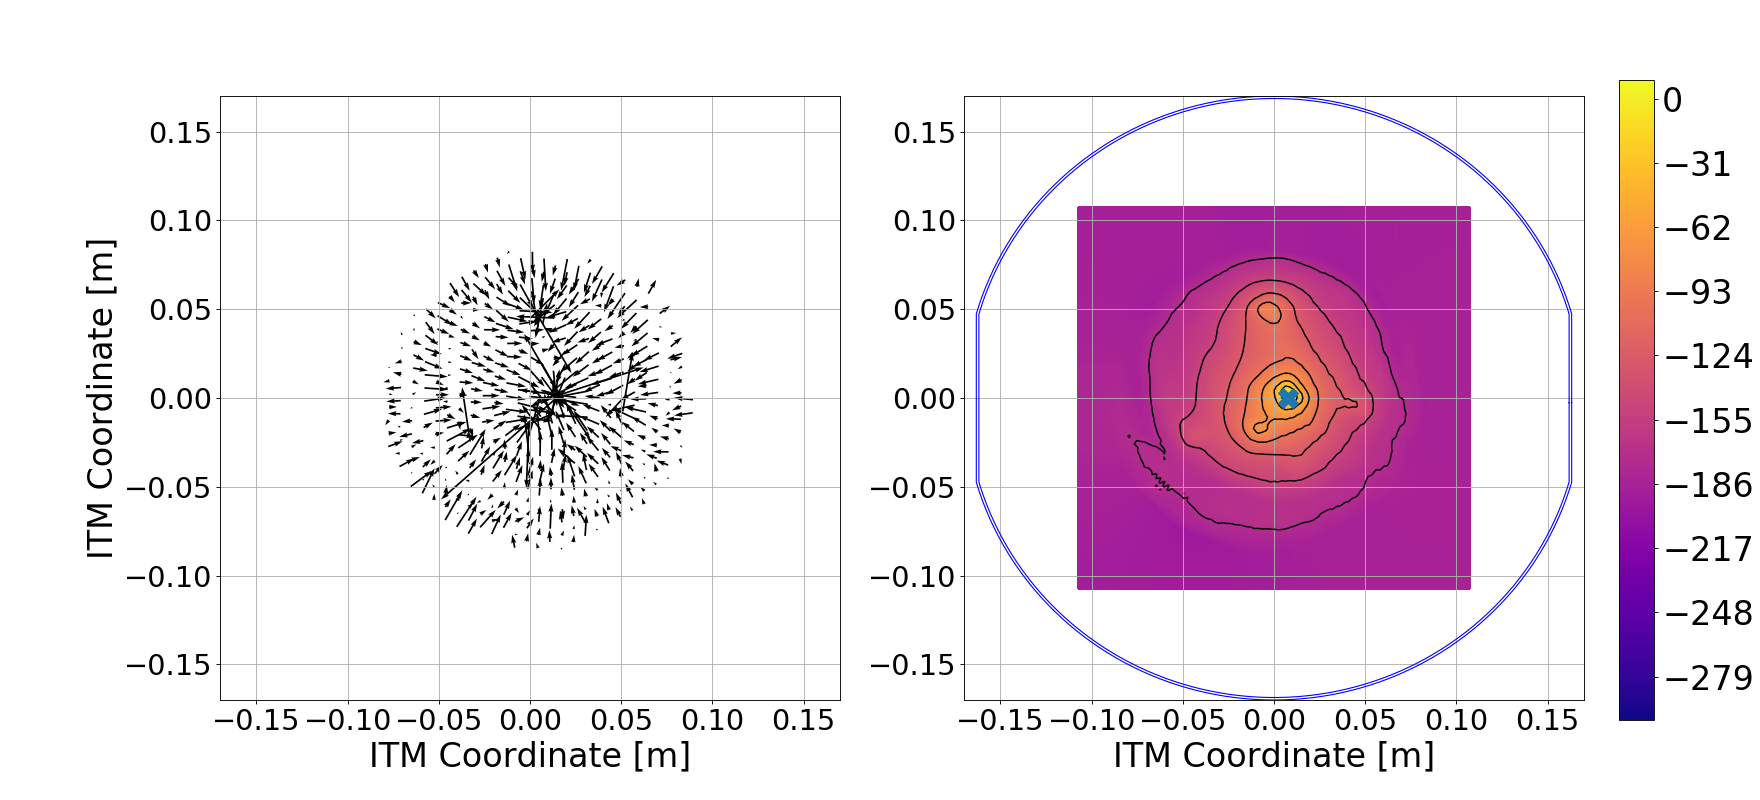
\includegraphics[width=0.55\textheight]{../Figures/1231726400_500dur_30W_ITMy.png}\quad
		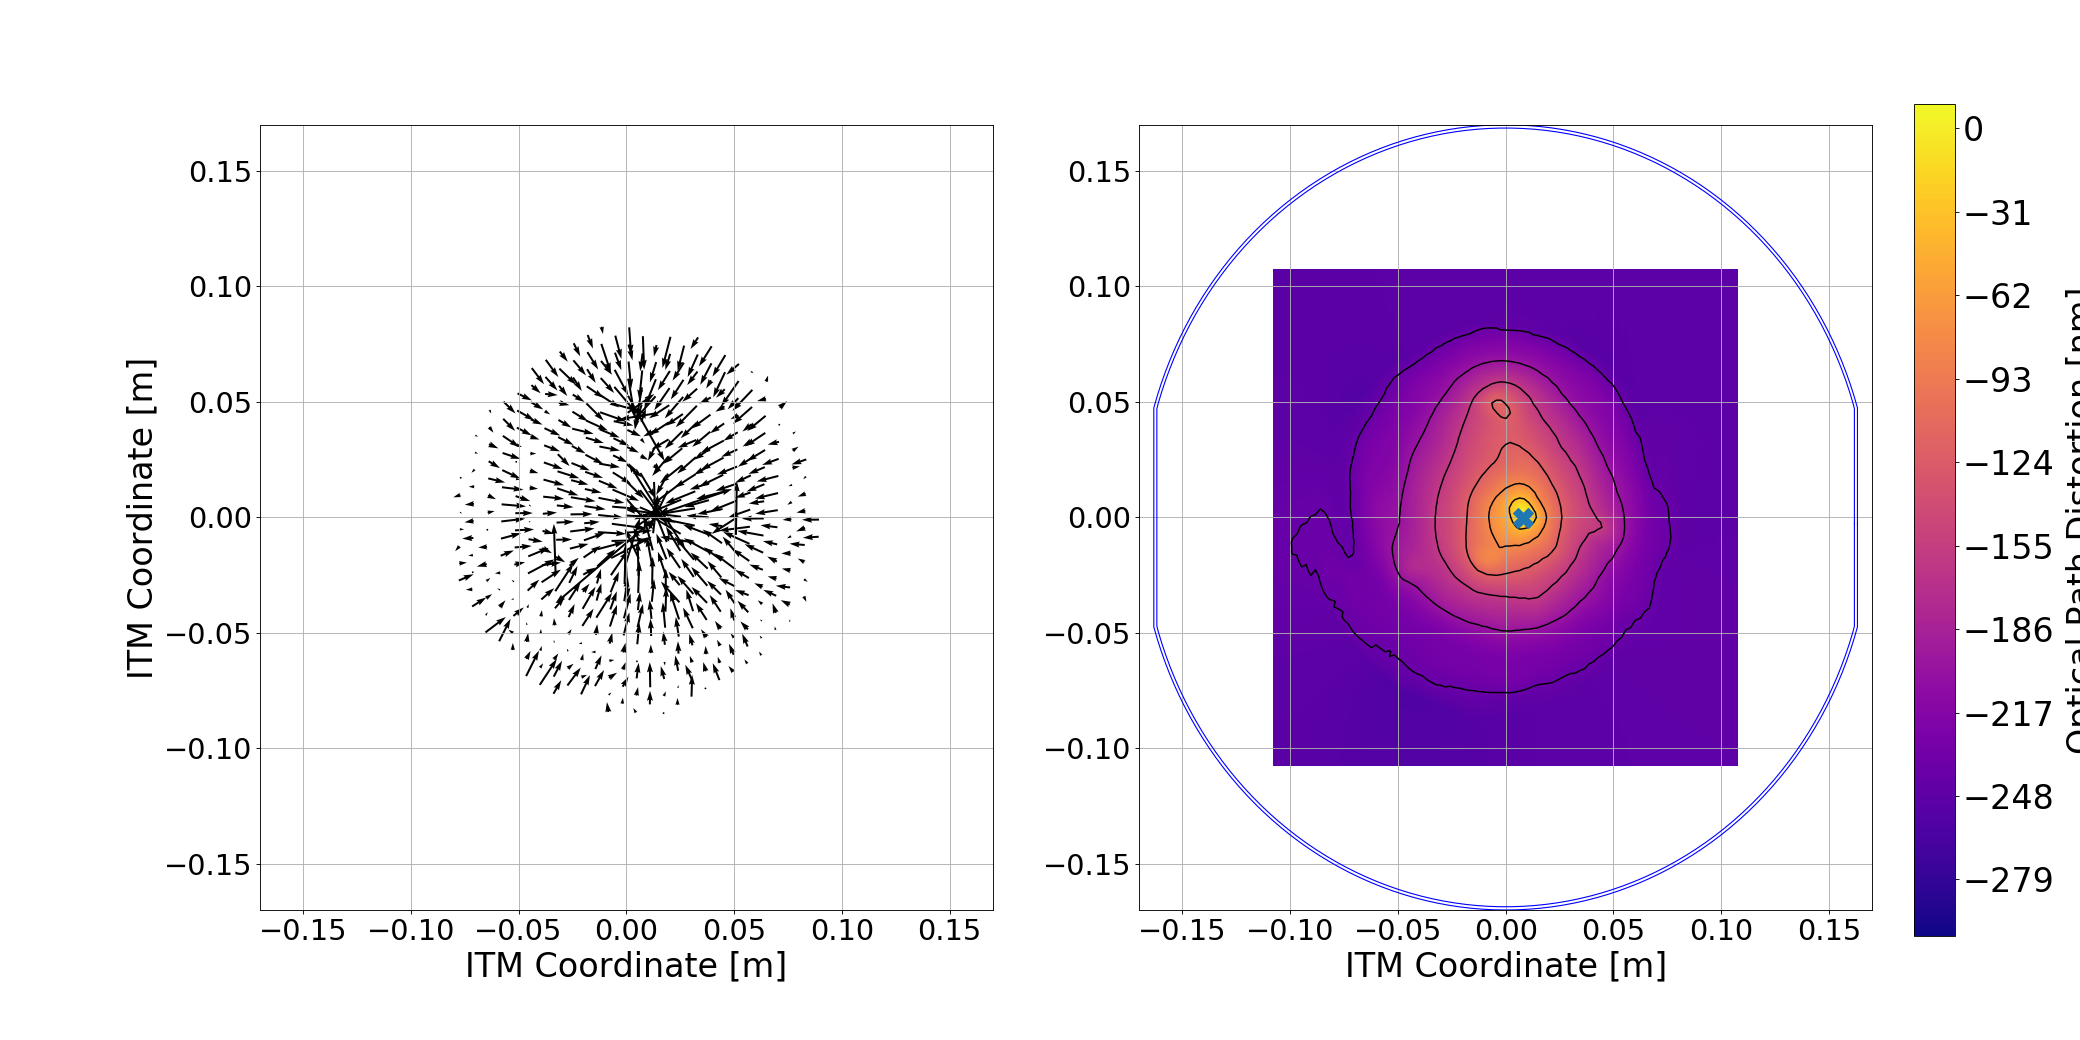
\includegraphics[width=0.55\textheight]{../Figures/1231726400_1000dur_30W_ITMy.png}\quad
		\caption[ITMY gradient plots (left) and wavefront maps (right) during a power up to 30 Watts of input power.]  
		{\textbf{ITMY gradient plots (left) and wavefront maps (right) during a power up to 30 Watts of input power.}
			Compared to the ITMX phase map in Figure \ref{fig:ITMX_HWS_plot}, ITMY has a much larger overall heating pattern and higher spatial frequencies in the contours which was the first clue that revealed multiple (possibly 4) point absorber on the test mass.  There is also a halo of gradients on the outer rim of the plots which is most prominent on the lower left corner.  This is due reducing the CO2 laser power in an attempt to compensate the lensing effects as the interferometer beam heats up the test mass.  The overall scale of self-heating with the higher spatial frequencies of the point absorbers makes it incredibly difficult to compensate with using the CO2 lasers as designed by Advanced LIGO. }
		\label{fig:ITMY_HWS_plot}
	\end{figure}

	\subsubsection{Measuring Uniform Absorption}
	After the arm power drops suddenly, the lensing decays exponentially depending on the amount of absorption on the high reflective surface of the arm cavity.  Using the HWS, it is possible to fit the decay rate to a finite element model of a cylindrical mass.  A fitted parameter for absorption is extremely important in pre-determining the amount compensation necessary to prepare the test masses for lock acquisition.  
	
	Applying an Markov Chain Monte-Carlo method allows some statistical uncertainty estimates for the exponential fitting to the data shown in Figure \ref{fig:mcmc_hws_abs}, where the priors are assumed to be random Gaussian noise and the initial guesses are scaled roughly with a least squares fitting algorithm. Figure \ref{fig:hws_abs} shows the measured spherical power from interferometer heating for ITMX/ITMY and comparing the two optics shows that the spherical power difference for ITMY is almost a factor of 2 larger than ITMX. One of the main differences between the O2 and O3 observing runs was the replacement of ITMX, ETMX, and ETMY test masses.  With a fully running Hartmann Sensor system in place which monitors the wavefront curvature across the optic, long-term trends over the observation runs will be able to determine how absorption changes as a function of time and whether test masses have an innate lifetime.  This will be particularly important if the next generation of detectors use much higher power levels in order to achieve better high frequency sensitivity \cite{DanBrown_prvt}.  Using this method, the current absorption estimates for the H1 input test masses are as follows:
	\begin{equation}
	\begin{aligned}
	A_{\text{ITMX}} &= 328 \pm 84 \; \text{ppb}\\
	A_{\text{ITMY}} &= 688 \pm 85 \; \text{ppb}
	\end{aligned}
	\end{equation}
	\begin{figure}[!]
		\centering
		\begin{subfigure}[a]{0.8\textwidth}
			\centering
			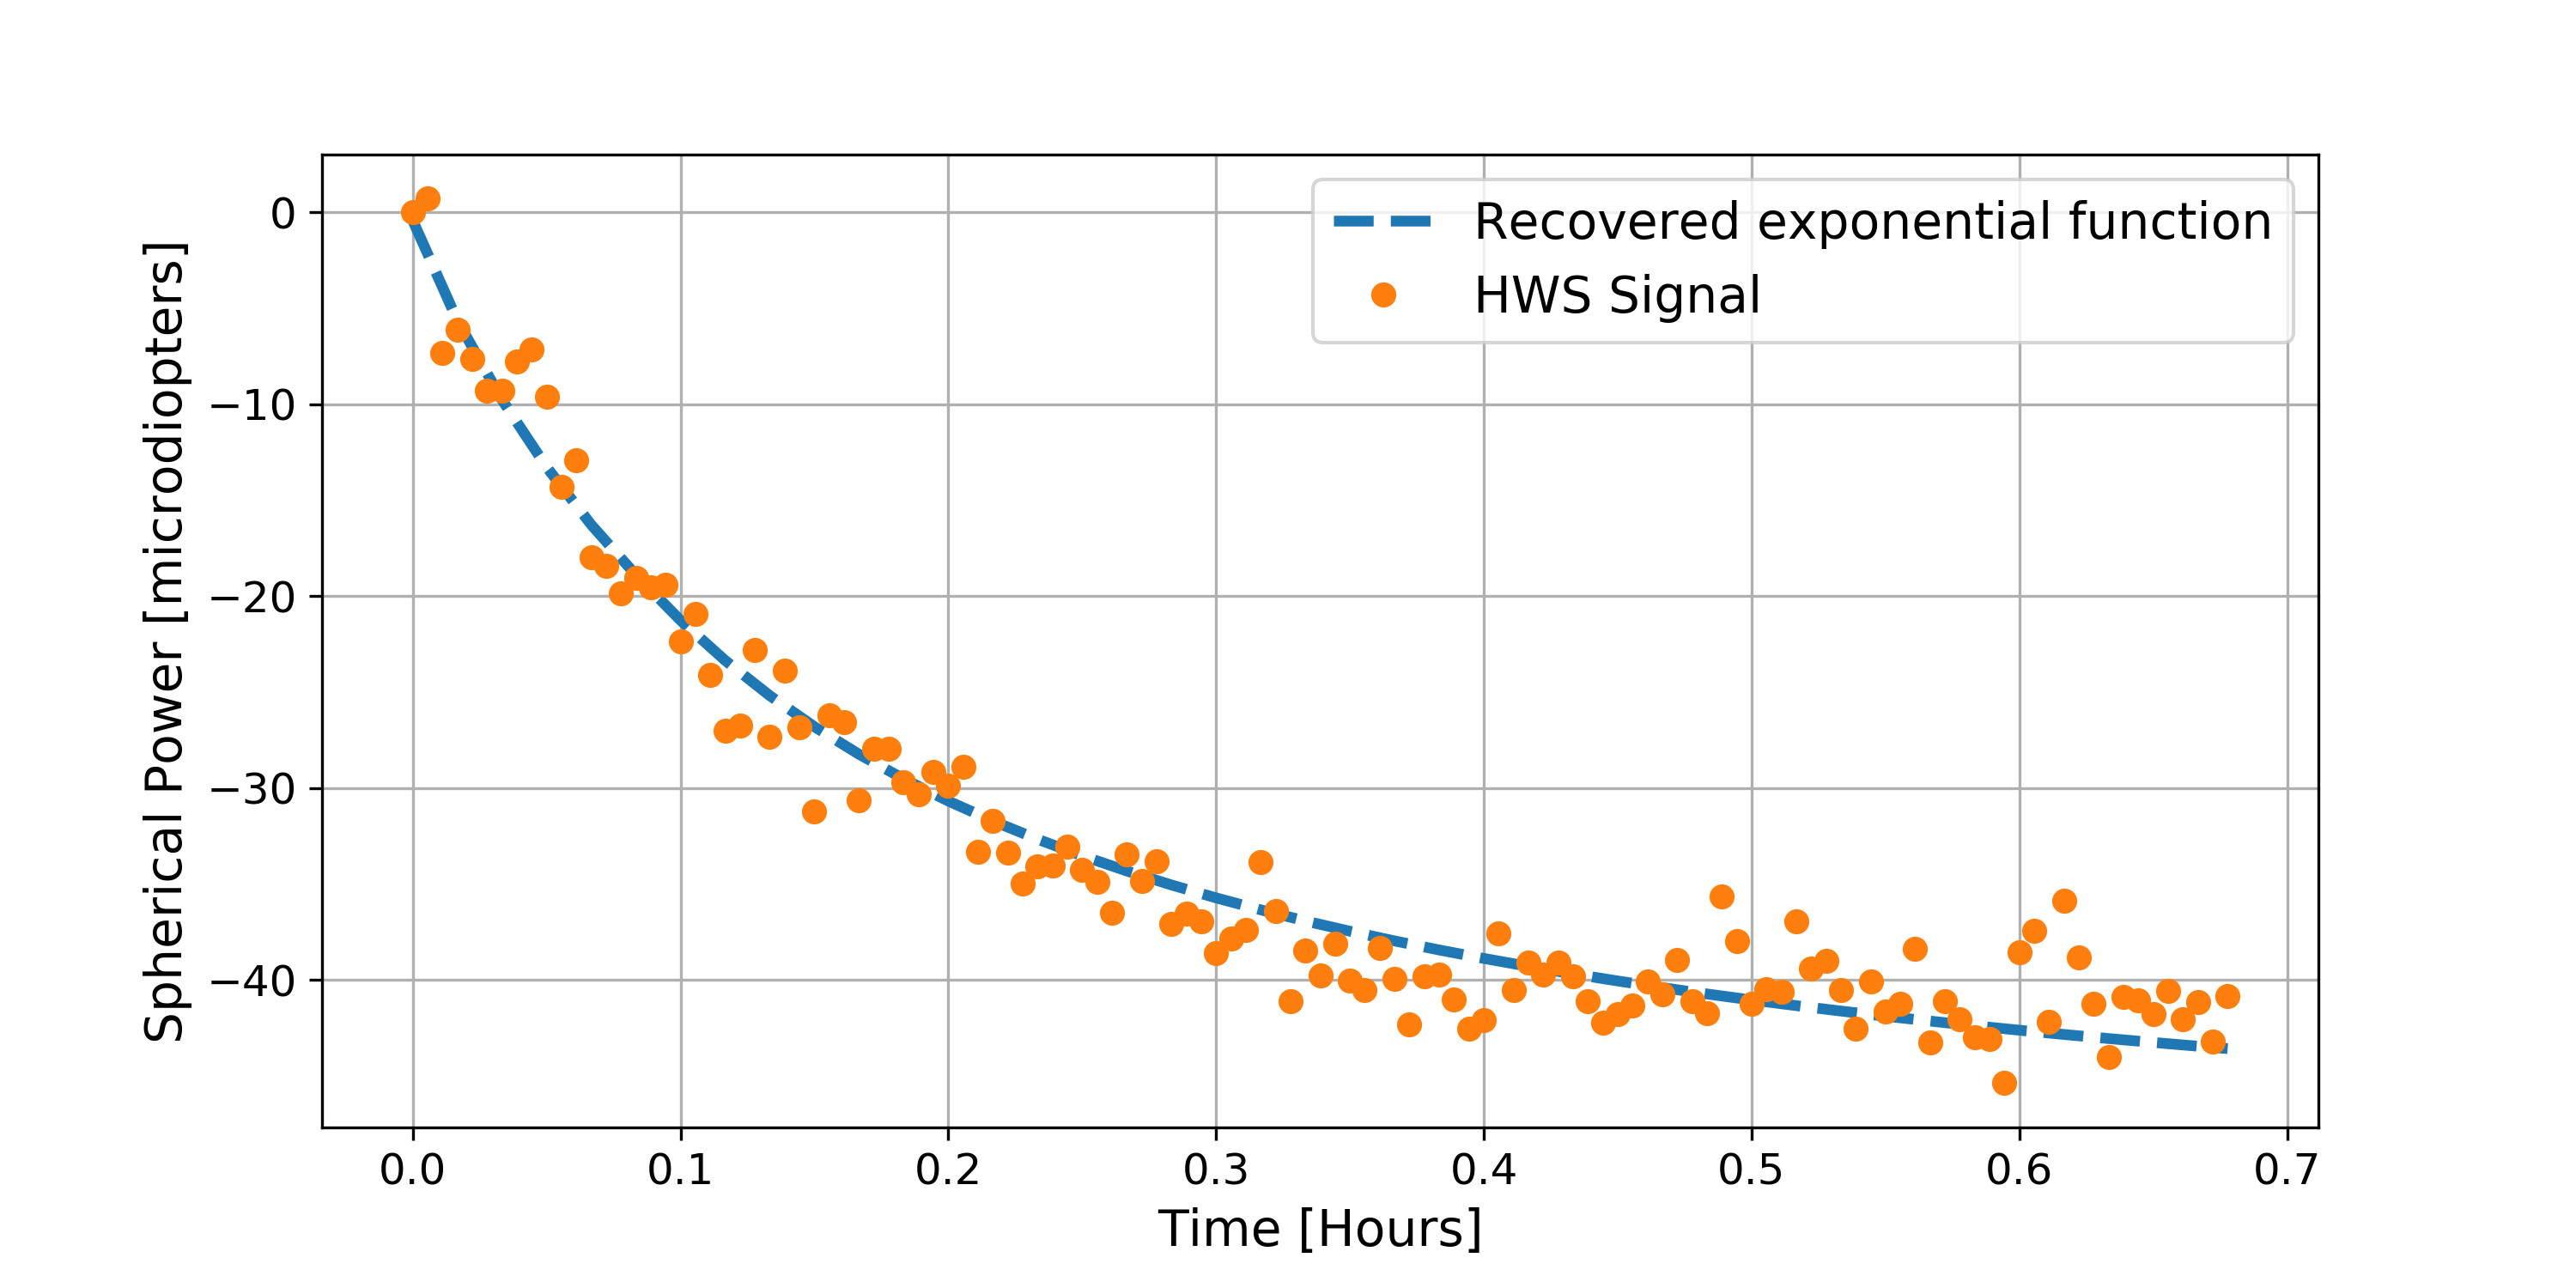
\includegraphics[width=\textwidth]{../Figures/MCMC_ITMX_ABS_FIT.png}
			\caption{ITMX absorption}
			\label{fig:itmx_abs}
		\end{subfigure}
		\hfill
		\begin{subfigure}[b]{0.8\textwidth}
			\centering
			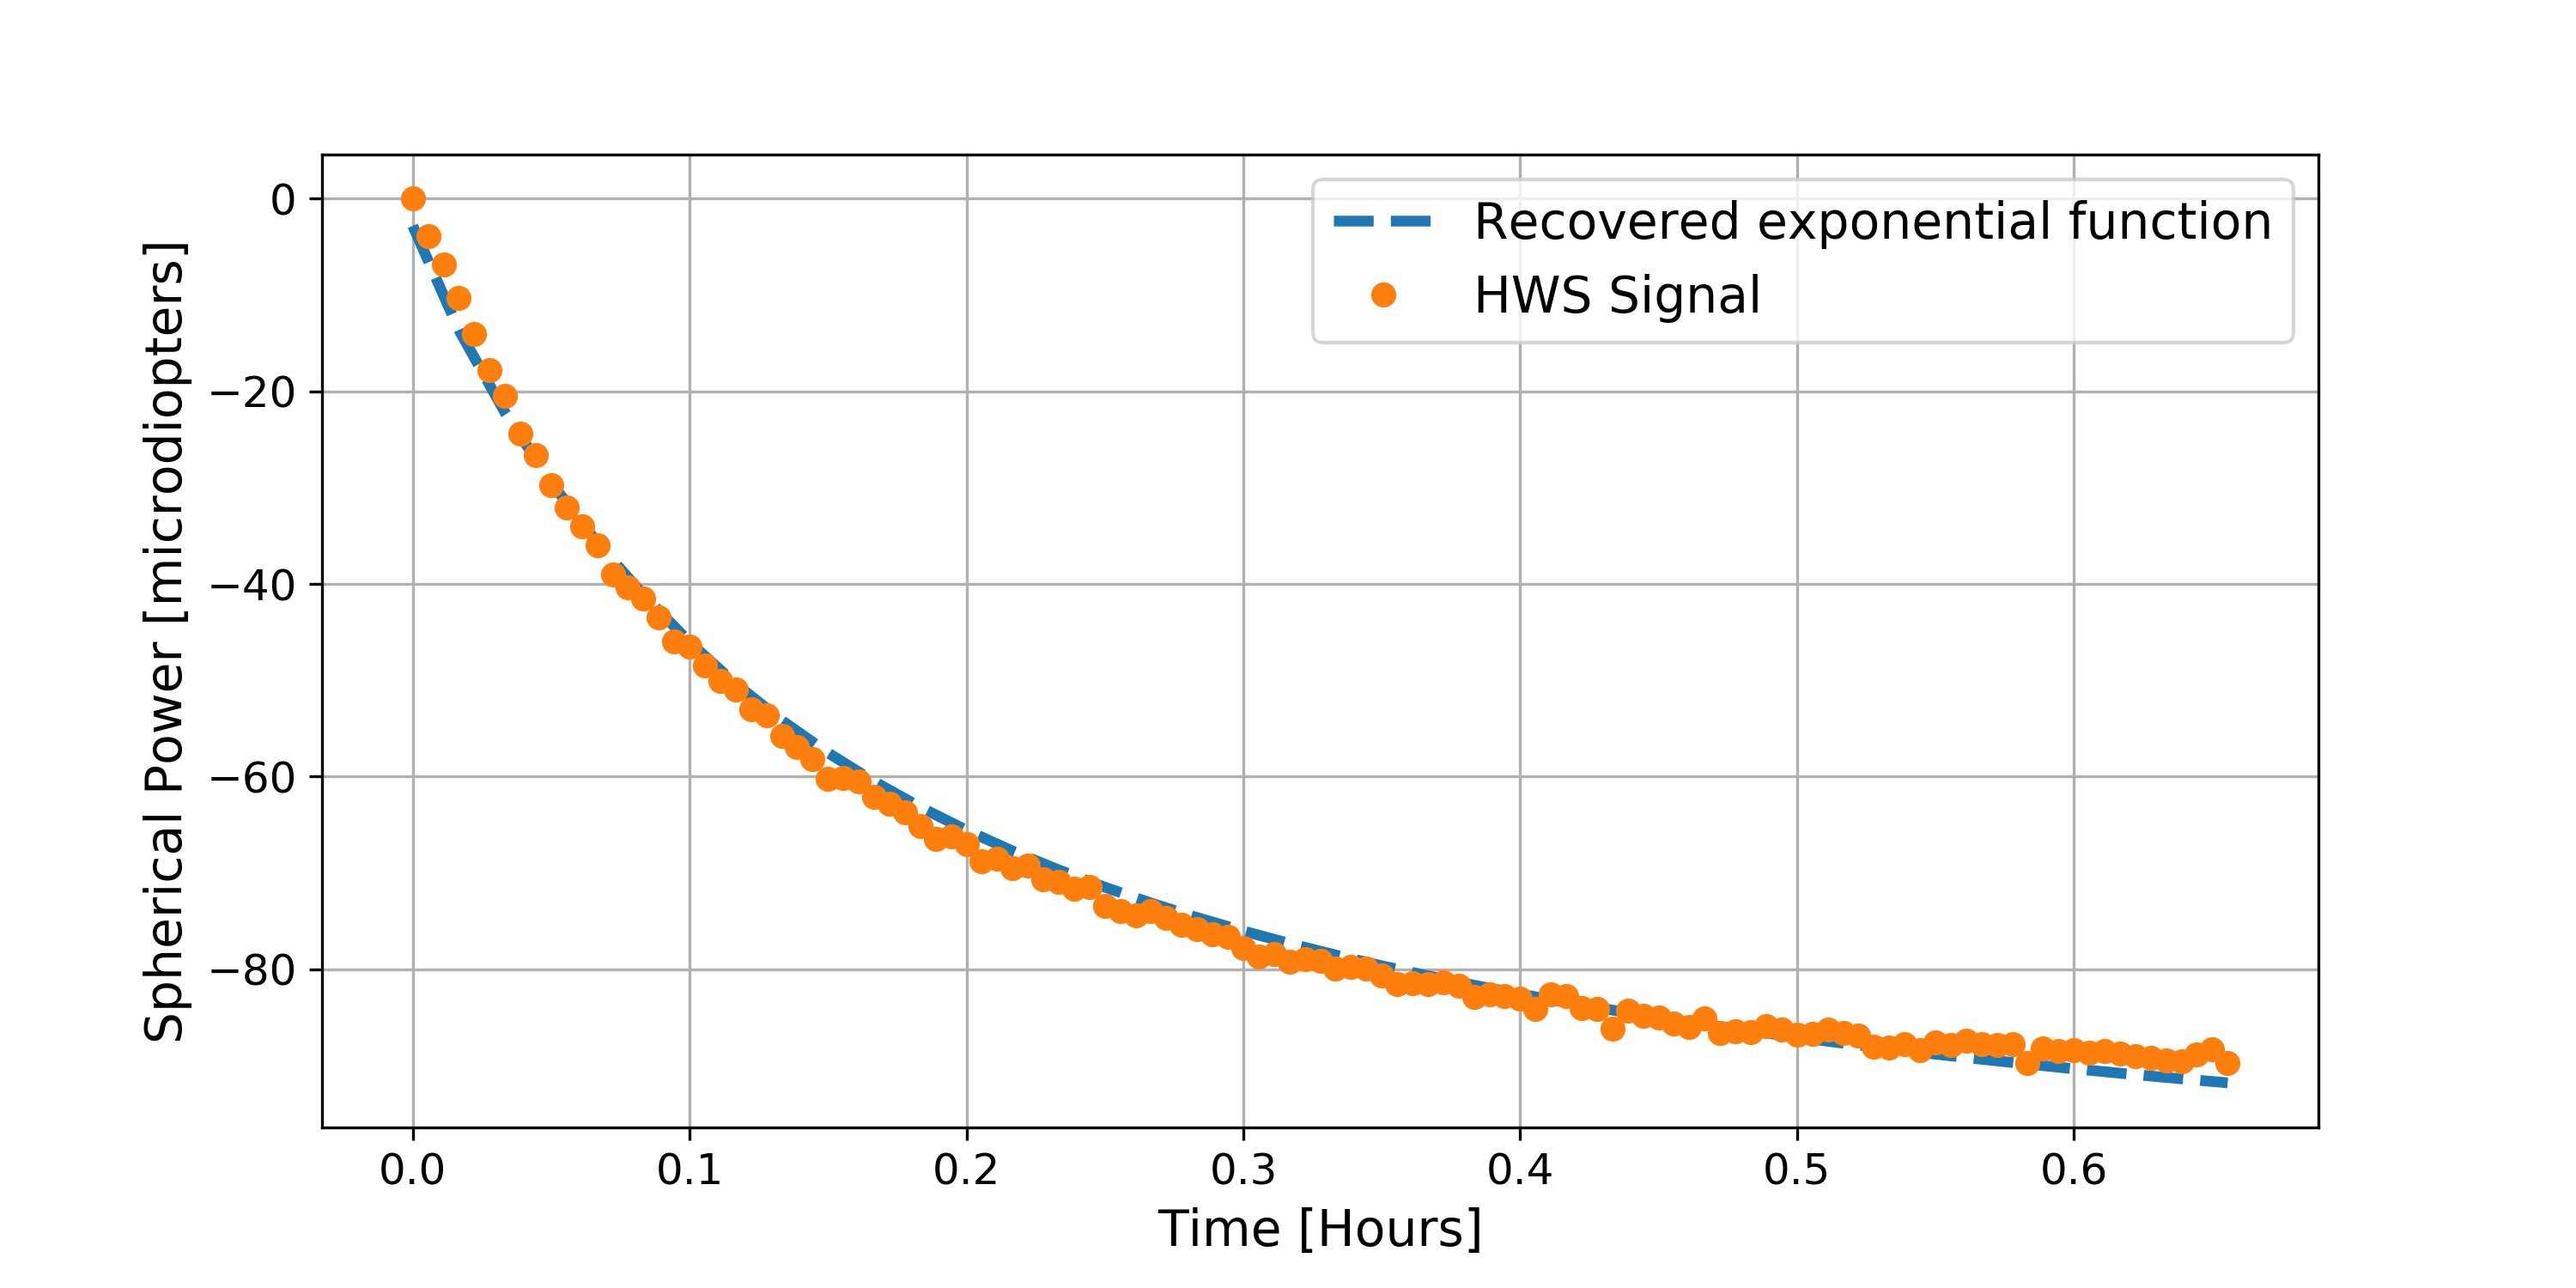
\includegraphics[width=\textwidth]{../Figures/MCMC_ITMY_ABS_FIT.png}
			\caption{ITMY absorption}
			\label{fig:itmy_abs}
		\end{subfigure}
		\caption[Thermal lensing as seen by the ITM Hartmann Sensors after a lock loss.]  
		{\textbf{Thermal lensing as seen by the ITM Hartmann Sensors after a lock loss.} A finite element simulation from COMSOL shows an impulse response which resembles an exponential decay can be linearized and fitted to the spherical power. The model assumes a beam size of 54 mm and 1 Watt of uniformly absorbed power then uses MCMC to fit the offset and scale to the data. Comparing ITMX and ITMY at Hanford shows a huge overall difference between the two optics, mostly due to the fact that ITMY has multiple point absorbers adding to the absorption estimate.  In addition, fitting ITMY data points with the model does not seem to agree very well which indicates extra physics that stems from non-uniform heating by a 54 mm beam.}
		\label{fig:hws_abs}
	\end{figure}
	
	\begin{figure}[!]
		\centering
		\begin{subfigure}[b]{0.5\textwidth}
			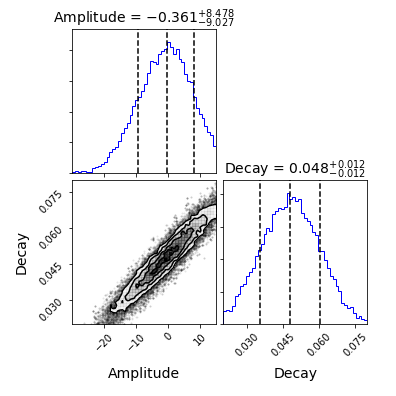
\includegraphics[width=\linewidth]{../Figures/MCMC_ITMX_abs.png}
			\caption{ITMX}
			\label{fig:mcmc_itmx_abs}
		\end{subfigure}%
		\begin{subfigure}[b]{0.5\textwidth}
			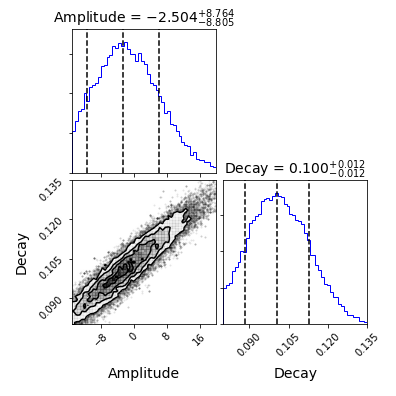
\includegraphics[width=\linewidth]{../Figures/MCMC_ITMY_abs.png}
			\caption{ITMY}
			\label{fig:mcmc_itmy_abs}
		\end{subfigure}
		\caption[Posterior distributions from fitting the Hartmann sensor spherical power.]  
		{\textbf{Posterior distributions from fitting the Hartmann sensor spherical power.}  
			Using the MCMC Hammer \cite{MCMC_Hammer}}
		\label{fig:mcmc_hws_abs}
	\end{figure}
	
	\subsection{Ring Heater and CO2 Commissioning}\label{Sec:RH}
	To counteract the effects of interferometer heating, Advanced LIGO uses a ring heater \cite{ramette_analytical} \cite{wang_thermalmodel} which has two heating elements mounted on the suspension cage. Each of them are glass formers wrapped by nichrome wire that has current running through it and radiates an annular heating pattern. The ring heaters will have two effects, it will induce a substrate lens and a radius of curvature change.  As shown in Section \ref{sec:hotcoldifo}, the carrier beam will not see the substrate lens but the radius of curvature difference will change the overall modal shape of the cavity.  Similar to the distortion derived in section \ref{sec:wf_dist} where the thermo-refractive effect dominates when dealing with a Gaussian beam, the same is true from the ring heaters. Using equation \ref{gauss_power_ovl}, one can directly calculate the power overlap between a pre-loaded cavity and the original, as it turns out, the effect varies the overlap by less than $0.1\%$

	After using the Hartmann sensors to determine the absorption and pre-loading the ring heaters to compensate the interferometer lensing, the substrate is no longer in the nominal configuration during lock acquisition.  Therefore, it is necessary to use CO2 (Carbon Dioxide) lasers to mimic the interferometer's heating on the compensation plate.  The CO2 lasers are located on each input test mass chamber and injected through a double zinc selenide viewport, then two steering mirrors direct the heating beam on the compensation plate of the reaction mass.  In initial LIGO, the CO2 beams were injected onto the high reflectivity surfaces of the test masses which created both a radius of curvature on the cavity side and a thermo-refractive change in the substrate.  However, in advanced LIGO, the CO2 lasers will only affect the substrate lensing.  Tuning the CO2 power will have a dramatic effect on the interferometer auxiliary degrees of freedom because the sidebands get rejected by the arm cavity and only resonate in the recycling cavities.  The self-heating caused by the interferometer beam is assumed to have a Gaussian intensity profile, while the CO2 heating beam is meant to have a uniform profile across the test mass surface which allows for a consistent phase distortion as a beam passes through the substrate.  Settings for the ITM ring heaters and CO2 lasers are calculated in Figure \ref{fig:TCS_ITMs} based off the Hartmann measurements.
	
	Determining the ITM ring heaters and CO2 power levels still leaves the end test mass ring heaters to be set.  In Figure \ref{fig:TCS_ETM}, the goal is to maintain the mode matching between the arms while simultaneously searching for the optimal overlap with the power recycling cavity.  This is done by determining the spatial mode overlap between all three cavities (XARM, YARM, and PRC). The linear portion of the graph shows a combination of common and differential adjustment of each ETM ring heater that keeps the mode matching between the arms at less than 1 PPM 
	
	\begin{figure}[!]
		\centering
		\begin{subfigure}[b]{1.0\textwidth}
			\centering
			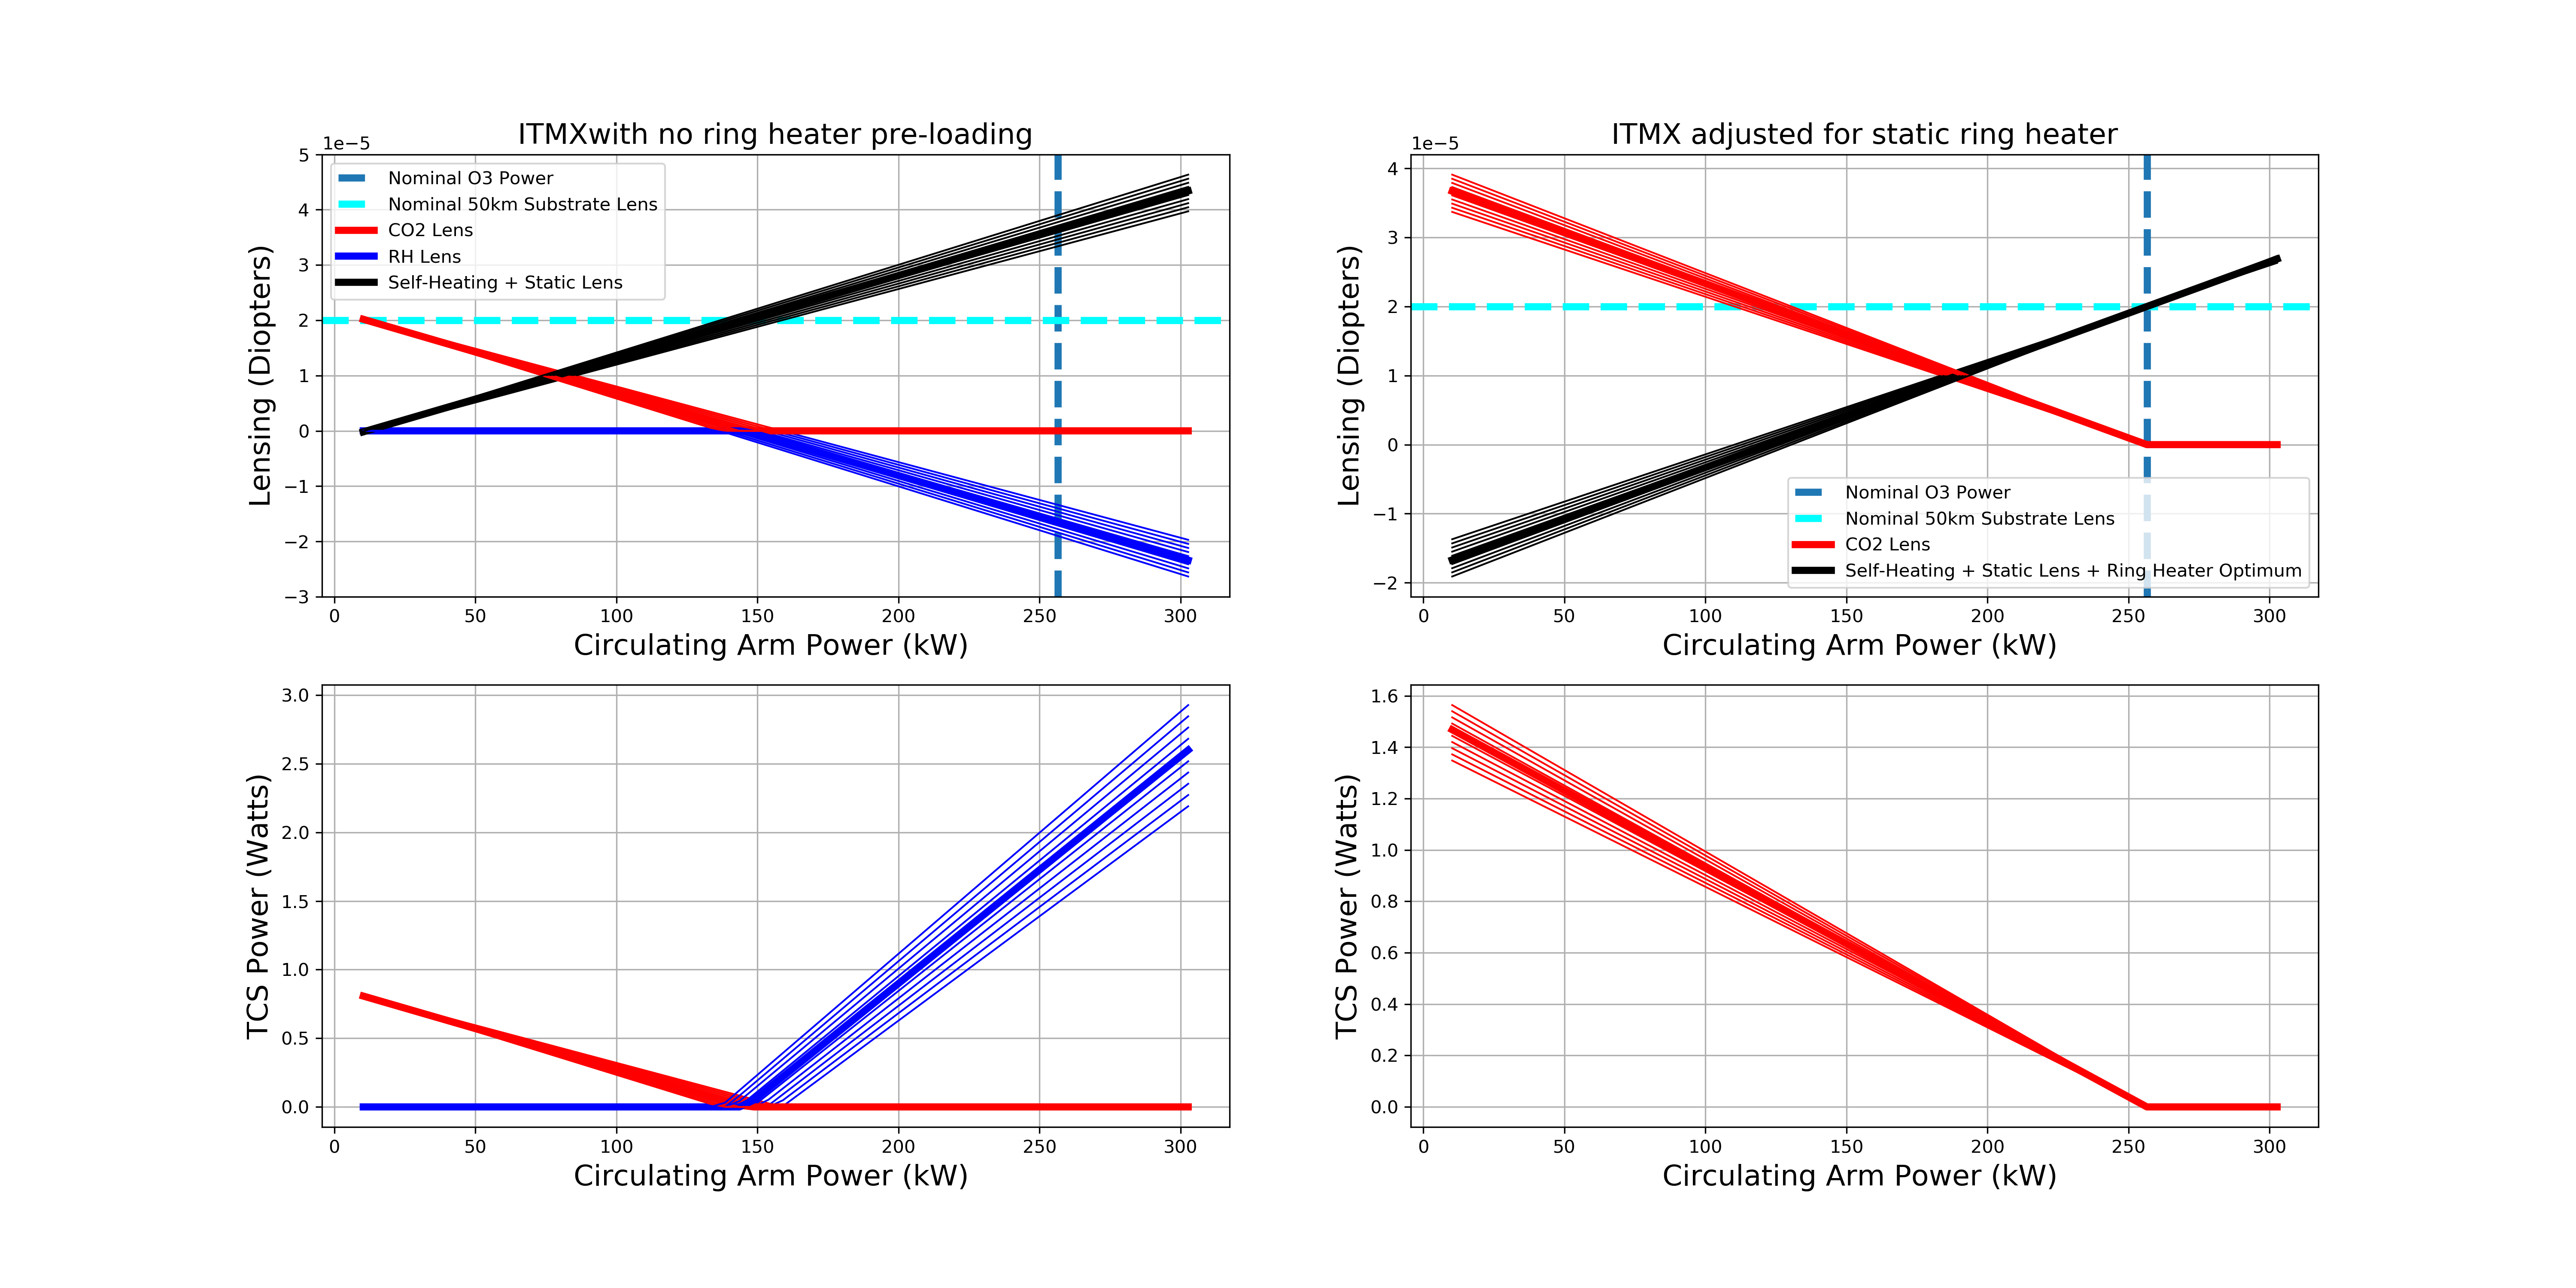
\includegraphics[width=\textwidth]{../Figures/ITMX_TCS_Settings.png}
			\label{fig:TCS_ITMX}
		\end{subfigure}
		\hfill
		\begin{subfigure}[b]{1.0\textwidth}
			\centering
			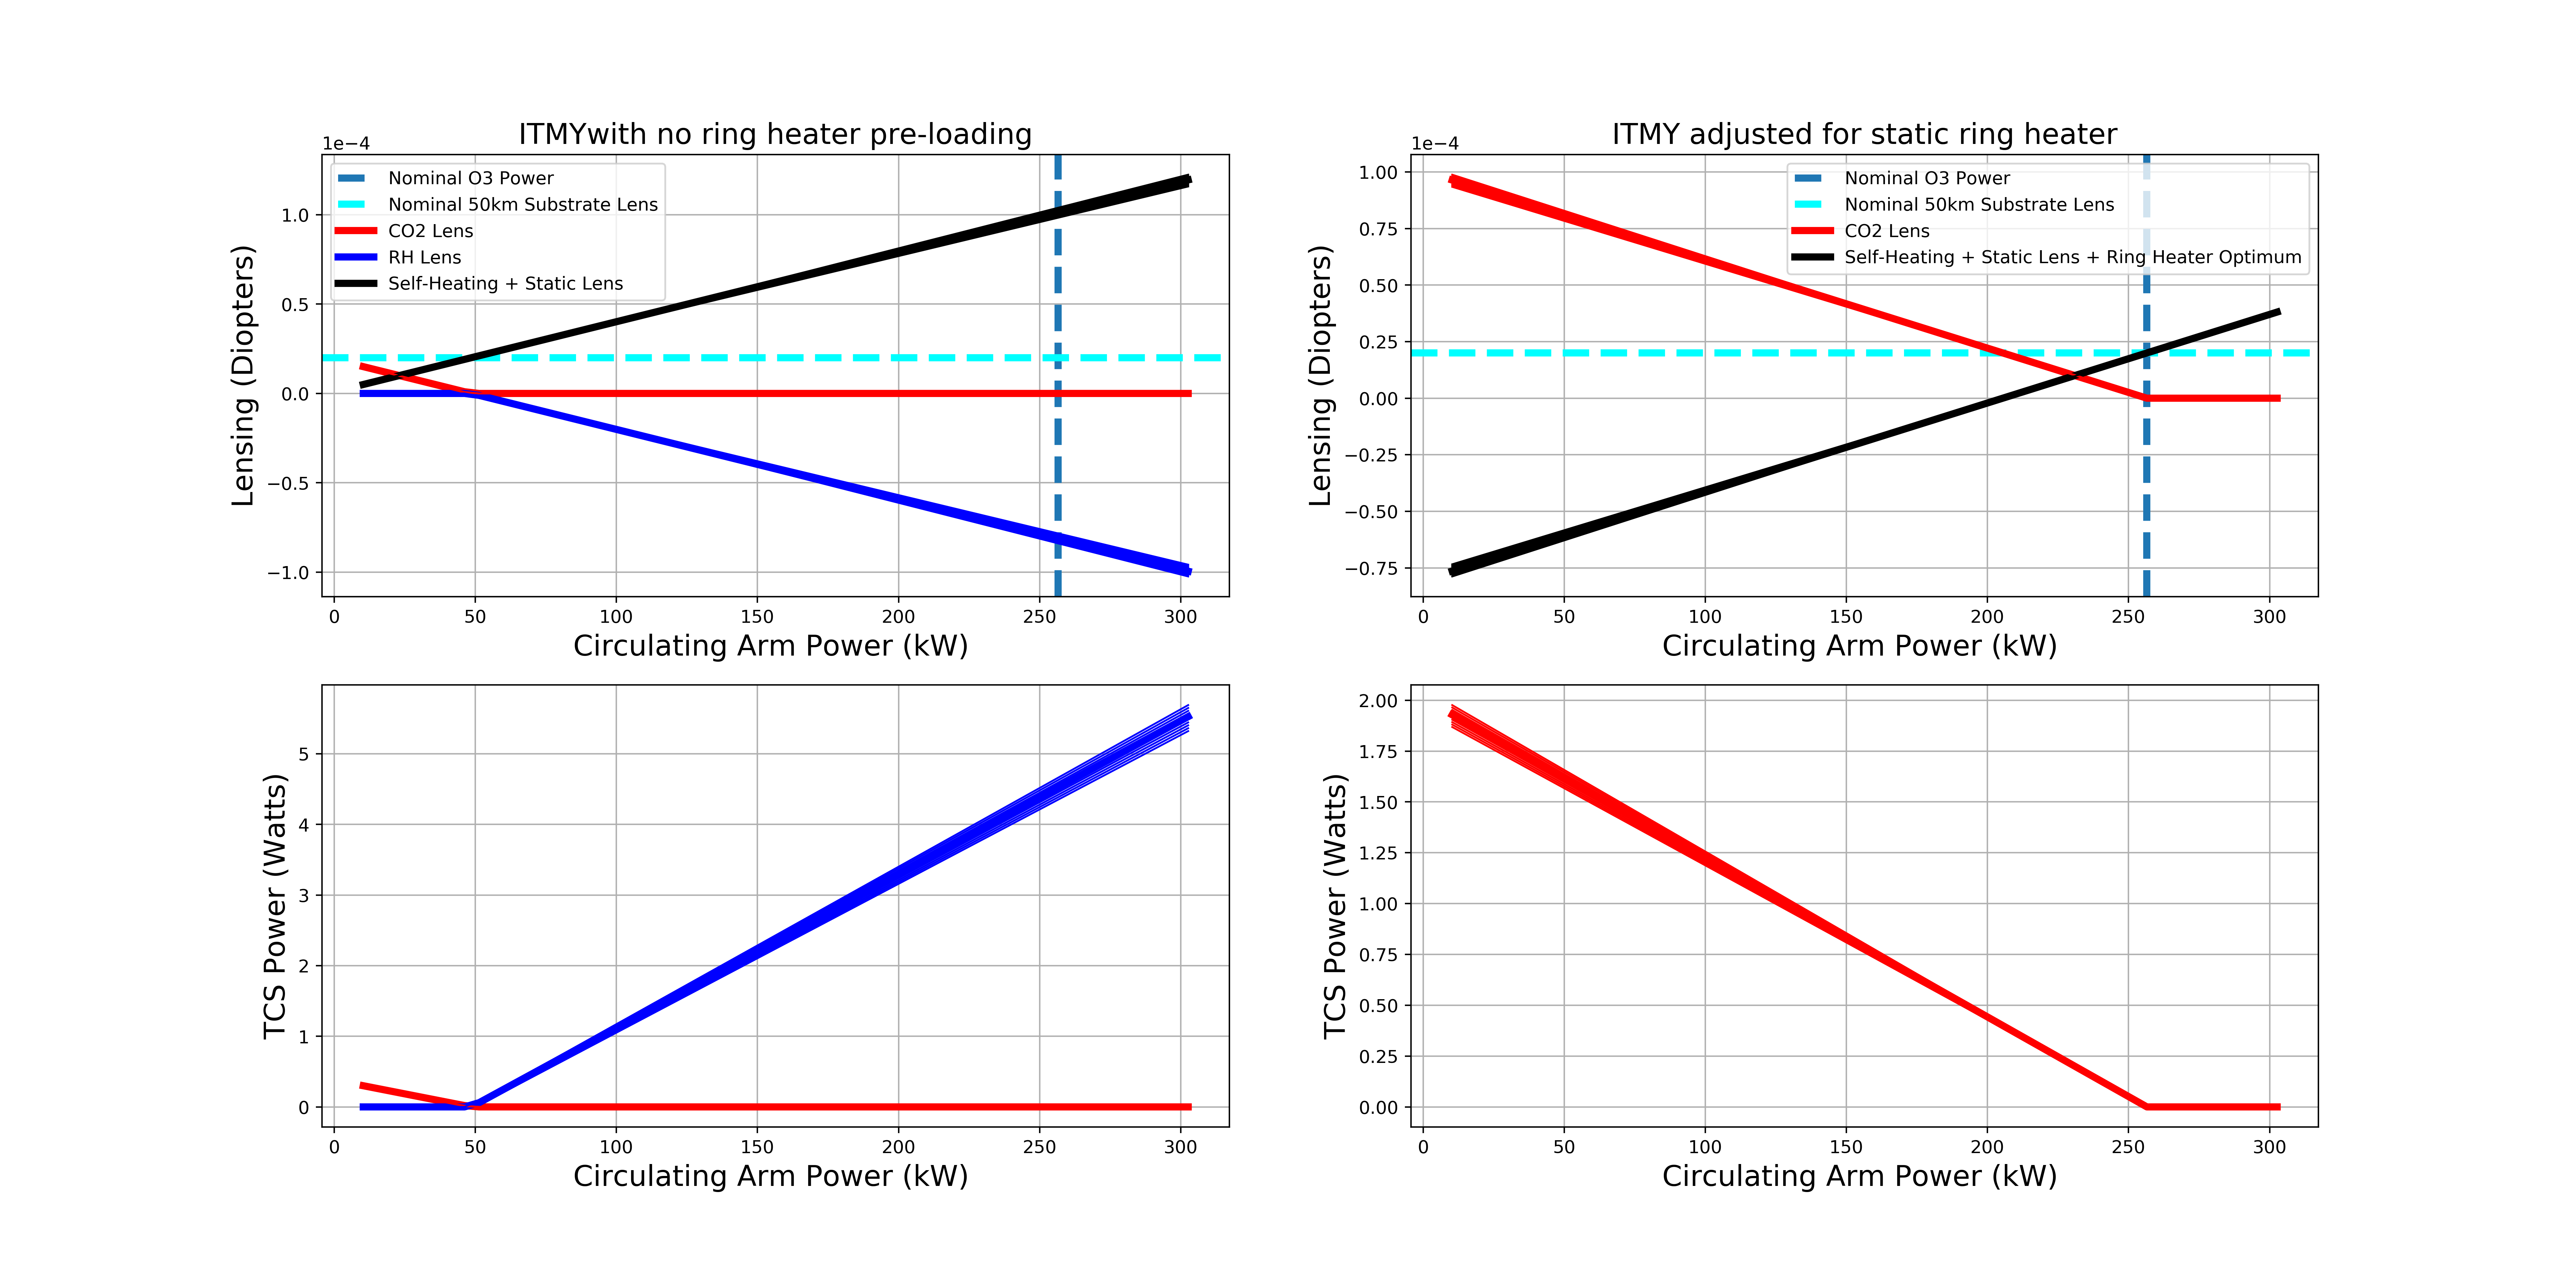
\includegraphics[width=\textwidth]{../Figures/ITMY_TCS_Settings.png}
			\label{fig:TCS_ITMY}
		\end{subfigure}
		\caption[Calculated TCS settings to balance the substrate lens.]{
			\textbf{Calculated TCS settings to balance the substrate lens.}  The nominal circulating power denoted by the vertical blue line is a function of the input power, the recycling gain, and the arm cavity gain.  The nominal input power for O3 will be 50 Watts and the power recycling gain is around 45.  The arm cavity gain can be estimated by calibrating the transmitted power from each of the arms and is approximately 228.  The horizontal, dashed turquoise line represents the nominal substrate lens with a focal length of 50 km.  This value is what the power recycling cavity expects to properly mode match to the arms. 
		}
		\label{fig:TCS_ITMs}
	\end{figure}
	
	\begin{table}[]
		\centering
		\begin{tabular}{|l||r|r|r|}
			\hline
			\hline
			& \multicolumn{1}{c|}{Substrate} & \multicolumn{1}{c|}{HR surface} & \multicolumn{1}{c|}{Compensation Plate} \\ \hline
			Self Heating & *4.9e-4                       & *-3.6e-5                        & N/A                                     \\ \hline
			Ring Heater  & -9.0e-6                       & *9.9e-7                         & N/A                                     \\ \hline
			CO2x         & N/A                            & N/A                             & 1.5e-5                                  \\ \hline
			CO2y         & N/A                            & N/A                             & 2.5e-5                                  \\ \hline
		\end{tabular}
		\caption[Single pass actuator lensing calibrations for aLIGO TCS in micro-diopters/Watt.] 
		{\textbf{Single pass actuator lensing calibrations for aLIGO TCS in micro-diopters/Watt.} The asterisks indicate the values are extracted from a model and the measured values use the Hartmann sensors which cannot distinguish between surface and substrate lensing, however, the latter is larger by an order of magnitude.  CO2x and CO2y were measured to be different in their actuation strength which could stem from either misalignment or a misplaced central mask.  The uncertainty is expressed by the last digit available.
		}
		\label{tbl:Actuaor_calibs}
	\end{table}
	
	\begin{figure}[!]
		\centering
		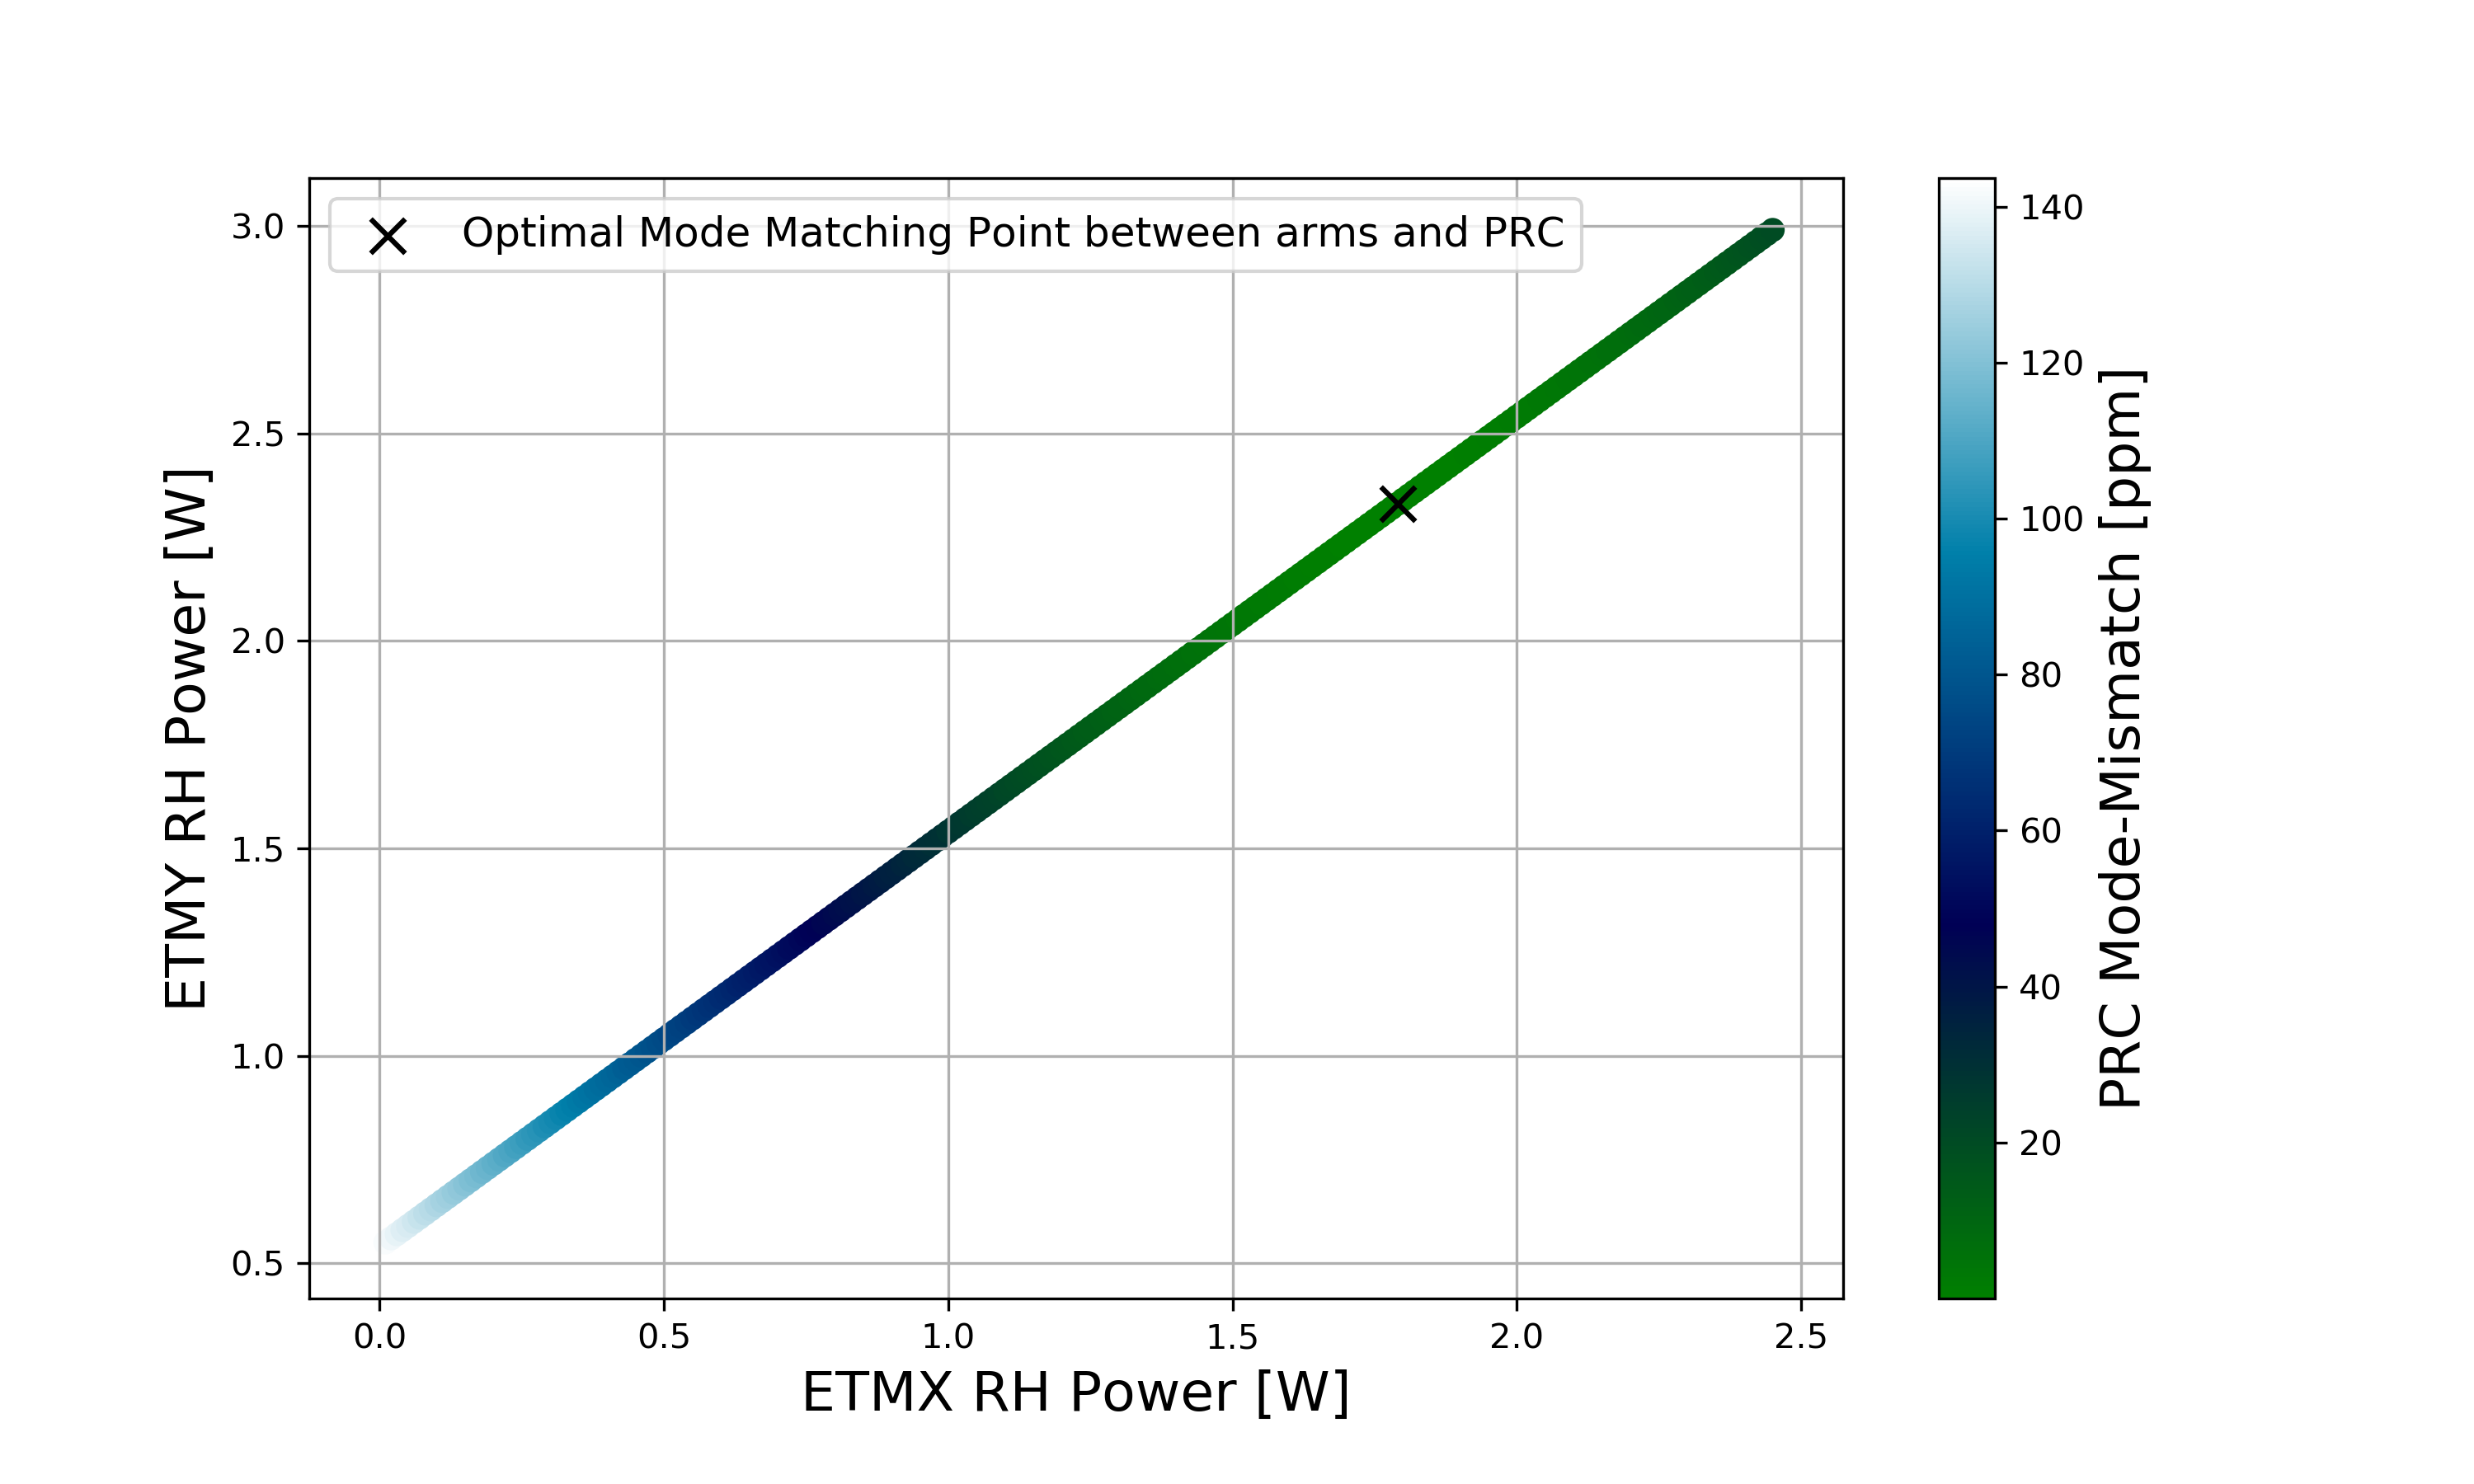
\includegraphics[width=1.0 \textwidth]{../Figures/ETM_TCS_Settings.png}
		\caption[Mode matching the arm cavities to the power recycling cavity.]{
			\textbf{Mode matching the arm cavities to the power recycling cavity.}
		}
		\label{fig:TCS_ETM}
	\end{figure}
\clearpage
\section{Point Absorbers}\label{sec:point_absorbers}
	Up till now, all actuators models, and measurements assumed uniform absorption across the optics which results in second order Hermite-Gauss coupling with the fundamental Gaussian beam .  As it turns out, this assumption is not so simple. One of the main successes for the Hartmann Wavefront Sensors have been the ability to find excess absorption due to point absorbers on the high reflectivity surfaces of the test masses.  During the second observation run (O2), there was an absorber found on ITMX that made increasing the input power past 30 watts extremely difficult and futile because it was thought to couple intensity noise into DARM. The exact origin of these point absorbers is still an active area of research but incursions into the vacuum system will always pose a risk of spreading particulate on the HR surfaces.

	\textbf{\emph{Part way into commissioning for O3, another point absorber on ITMY was detected that showed similar characteristics.}}  Since their spatial frequencies are much higher than the uniform absorption, many of the models for scattered power and thermal effects require significant adjustment to predict the interferometer behavior.  To decompose the differential phase map into the Hermite Gauss basis requires a relatively high order and makes full interferometer simulations very difficult.  For example, FINESSE calculations on a laptop tend to become unwieldy at around $n+m = 6$.  This affects the HWS's ability to properly evaluate total thermal lens from the interferometer, therefore changing the estimated absorption.  There are two main parts which allow point absorbers to adversely affect interferometer performance.   The first is scattering from the arm cavity that takes away carrier light and couples to higher order modes, and secondly, the thermal lens in the substrate distorts the power recycling cavity for the sideband build ups dramatically.
	
	A few ways to try getting around this could be separating the temporal effects which quadratically depend on the point absorber size. The thermo-refractive transient solution found in Vinet \cite{Vinet_Thermal_Issues} has the form
	\begin{equation}\label{Thermal_Dist_time}
	Z_{\text{TR}}(t)   \propto 1-\exp{-t/ \tau}
	\end{equation}
	where $\tau = \frac{\rho C w_\text{pa}^2}{3 \kappa} $ is the characteristic time constant that depends on the beam size $w_\text{pa}$, the thermal conductivity $\kappa$, the specific heat $C$ and the material density $\rho$.  A simple model can consist of two beams with different sizes which will have separate time constants.  Another interesting way of characterizing what can be compensated for O3 could be to Fourier transform the optical path distortion and low pass the high spatial frequency components with a Gaussian filter. The cut-off frequency can be estimated by the approximate point absorber size (10-20 mm).  Of course, early detection and replacement of an optic may be the most efficient way to avoid custom thermal compensation.  Figure \ref{fig:3d_HWS_plot} shows a comparison between ITMX and ITMY while the interferometer is increasing input laser power from 2 to 30 Watts.  Within the first few hundred seconds, the point absorbers begin showing up in the optical path distortion map.
	
	An interesting coupling that was discovered which the point absorbers could be responsible for is higher order mode 9 Mhz leakage through the OMC.  Generally, the OMC is very good at rejecting both the sidebands and first few higher order modes but the addition of point absorbers couples greater spatial frequencies than anticipated.  Careful analysis by Koji Arai \cite{9rin} shows the Hanford OMC can allow some 9th order 9 Mhz onto the OMC DCPDs.  This coupling should provide a decent metric for reducing the point absorber induced noise. 
	
	During commissioning periods, the highest starting priority is to achieve full resonance as quickly as possible and is easier with approximately 2 Watts of input laser power. This requires locking the arm length stabilization (ALS) system with 532 nm, the vertex degrees of freedom (DRMI) and complete the common arm length (CARM) transition. Additionally, closing all angular degrees of freedom (ASC) will take a lot of time and energy.  If major upgrades or fixes have occurred such as replacing main test masses then all the prior steps require many months of commissioning.  Generally, vacuum incursions into the main vertex cost the most time and money because of the large volume needing to be pumped.  All this is to say, the earlier point absorbers are detected, the better.  However, this requires a high level of arm power which historically has come much later on the road to nominal low noise.  In Figure \ref{fig:HWS_spectra}, the signal-to-noise ratio is 10 at 0.01 Hz for 37.5 mW of absorbed power which means the circulating arm power must reach at least 75 kW  (assuming absorption is approximately 0.5 ppm)to be detectable within the time constant of point absorbers. This could still be achieved without full lock if the first priority after pumping down is resonating a single arm with power recycling at the highest input laser power possible (currently 70 Watts).  With a single power recycled arm cavity the expected circulating power absorbed on the HR surface of the test masses is
	\begin{equation}
	\begin{aligned}
	P_\text{PRC-1ARM} &= P_{\text{in}} * g_{\text{PRC}} * g_{\text{ARM}} * 0.25 * \epsilon_a\\
	&\approx 98 \; mW \; \bigg[\frac{P_{\text{in}}}{70 \, \text{Watts}}\bigg] \; \bigg[\frac{g_{\text{PRC}}}{ 45 }\bigg] \; \bigg[\frac{g_{\text{ARM}}}{ 225 }\bigg] \; \bigg[\frac{\epsilon_a}{0.5 \, \text{ppm}}\bigg]
	\end{aligned}
	\end{equation}
	where the factor of 0.25 comes from double passing the main beamsplitter, the coefficient $\epsilon_a$ is the estimated uniform absorption.  Using $ D_{\text{sub}} \approx 487 \frac{\mu \text{D}}{1 \; \text{Watt}}$ as the modeled conversion from absorbed power to steady-state spherical power, the expected substrate lensing in units of micro-diopters [$\mu \text{D}$] is
	\begin{equation}
	S_\text{PRC-1ARM} = P_\text{PRC-1ARM} *  D_{\text{sub}} \approx 48 \mu\text{D}
	\end{equation}
	 which readily detectable by the current Hartmann sensors. Commissioning and installation schedules are ever-changing entities and there have been times when the end stations are not ready for integration simultaneously. This provides a window where only single arm commissioning is available so this method might be able to detect the existence of point absorbers much sooner.
	 
	 \indent Once these anomalies are found, the question remains, what can be done?
	 
	 One consideration is a complete re-design of Thermal Compensation to account for higher frequency spatial corrections. There are already custom masks at Hanford which are designed to smooth the optical path distortion in the substrate and can be implemented with the CO2 lasers on the compensation plate to increase the sideband build ups, which is one of the biggest difficulties associated with point absorbers.  However, this does not solve the fundamental problem of losing power recycling gain due to power scattering where the quadratic losses of the arm cavity set an upper limit for increasing power.  Another way to avoid these effects is to move the beam spot away from the point absorber on the HR surface but it must be sufficiently far or the odd higher order modes will couple very strongly with asymmetry. These two strategies are not necessarily orthoganal since moving the spot position changes the required correction mask.
	 
	 In terms of noise, the 9 Mhz RIN coupling to the OMC DCPDs could be reduced with changing the OMC transverse mode spacing by locking on a different carrier resonance a free spectral range away.  The introduction of a well-tuned custom mask should also reduce higher order mode content in the recycling cavities.
	 
	 \begin{figure}[t!]
	 	\centering
	 	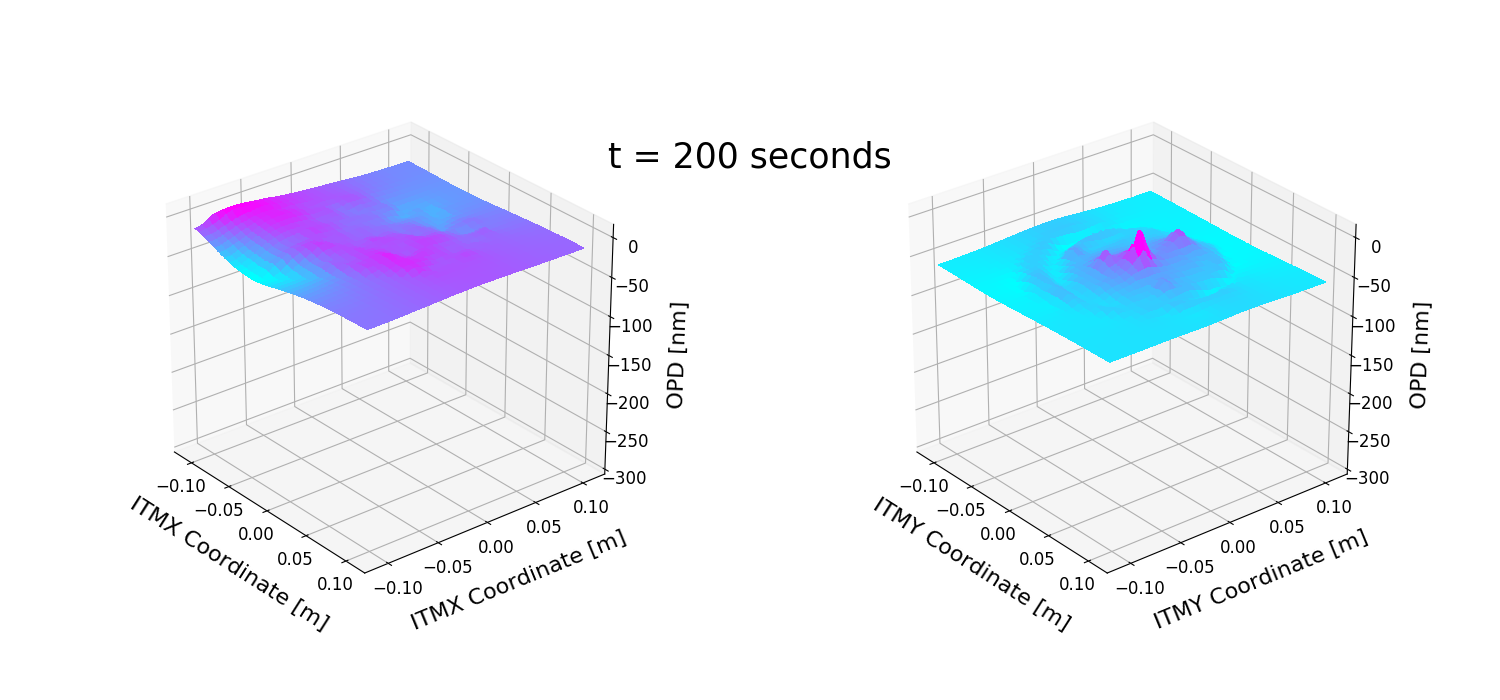
\includegraphics[width=0.4\textheight]{../Figures/1231726400_3d_200dur_30W_ITM.png}\quad
	 	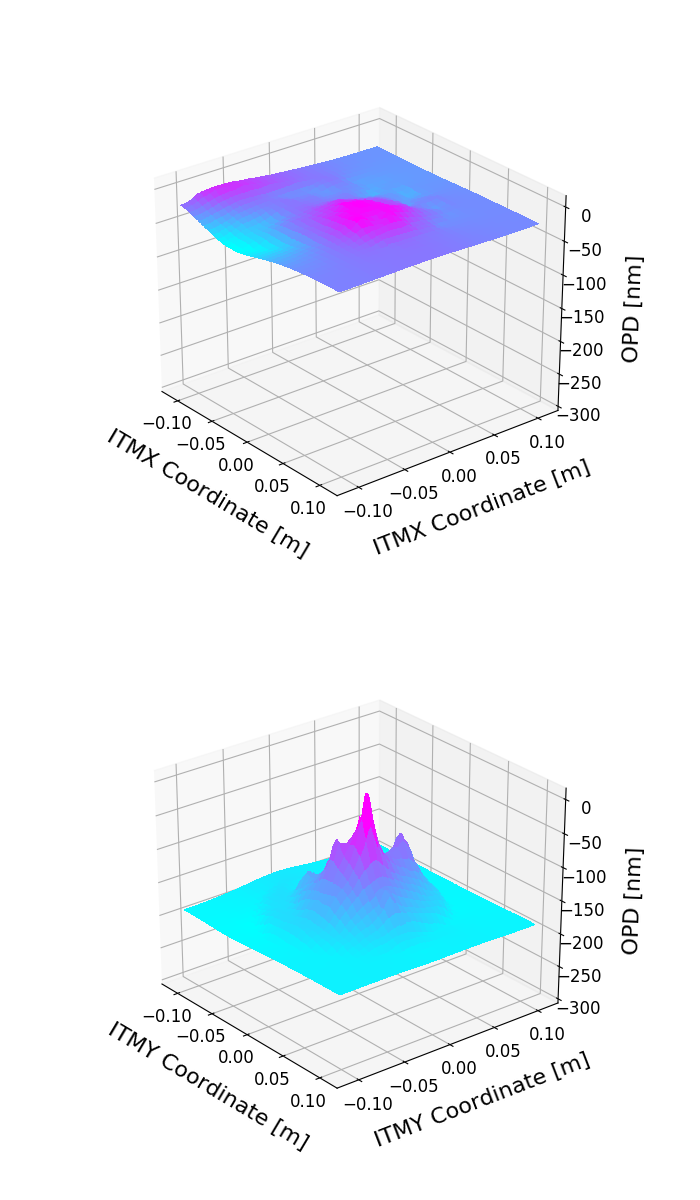
\includegraphics[width=0.4\textheight]{../Figures/1231726400_3d_500dur_30W_ITM.png}\quad
	 	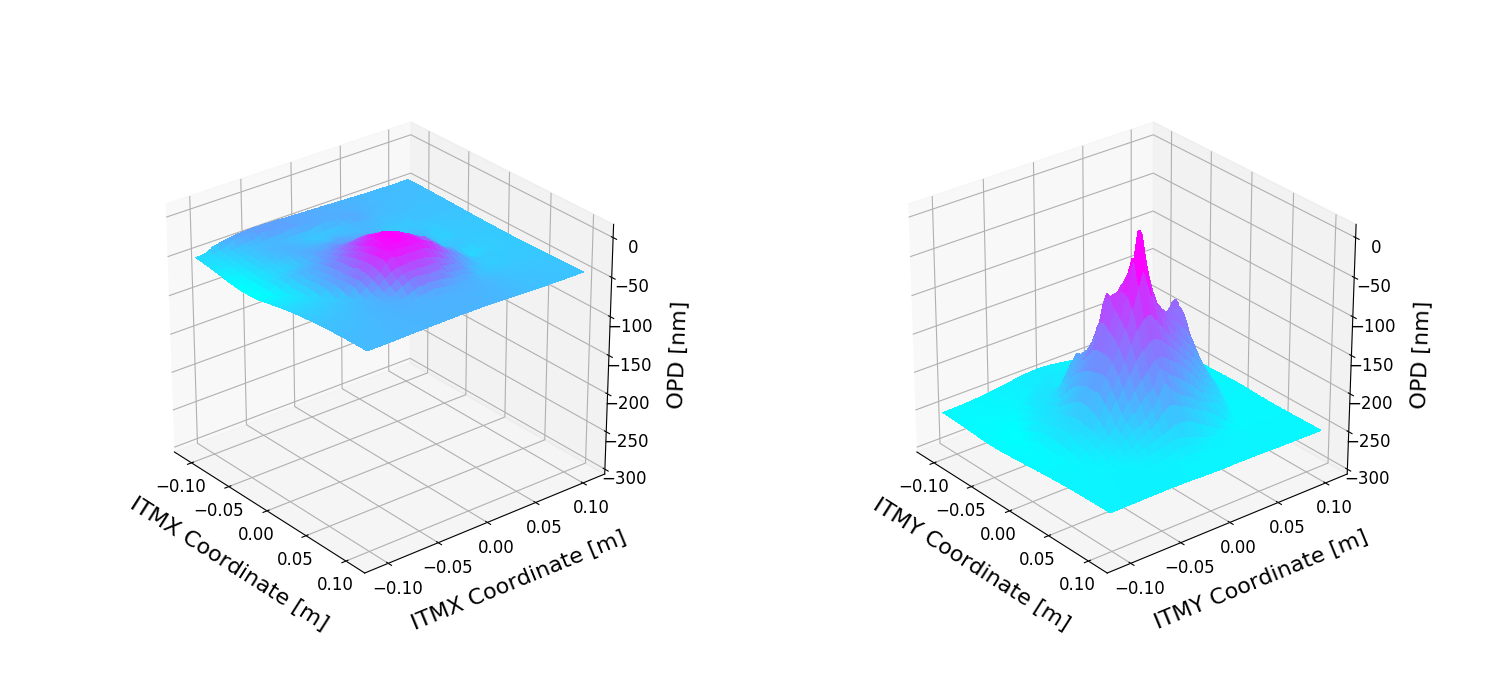
\includegraphics[width=0.4\textheight]{../Figures/1231726400_3d_1000dur_30W_ITM.png}\quad
	 	\caption[Comparing 3-D plots of the optical path distortion for ITMX and ITMY test masses after powering up the interferometer.]  
	 	{\textbf{Comparing 3-D plots of the optical path distortion for ITMX and ITMY test masses after powering up the interferometer.}
	 		The horizontal axes represent the test mass coordinates as seen on the Hartmann sensors and the vertical axis is the optical path distortion in units of nanometers. The color map is scaled for each plot and is meant to show particularly hot areas and roughly compare the high frequency spatial distribution of point absorbers. Plots in the left column (ITMX) have smooth spatial features that stem from uniform absorption and the effects are not prominent till after approximately 500 seconds.  In contrast, plots in the right column (ITMY) have very sharp spatial features which already rise above the floor at 200 seconds into powering up.  Comparing the overall surface deformation on the same scale, the difference between ITMX and ITMY is striking and it is clear how an interferometer with point absorbers on the surface will struggle to increase powers above 200 kW within the arm cavities.
	 	}
	 	\label{fig:3d_HWS_plot}
	 \end{figure}

	\begin{sidewaysfigure}[t!]
		\centering
		\begin{minipage}{0.5\textheight}
			\centering
			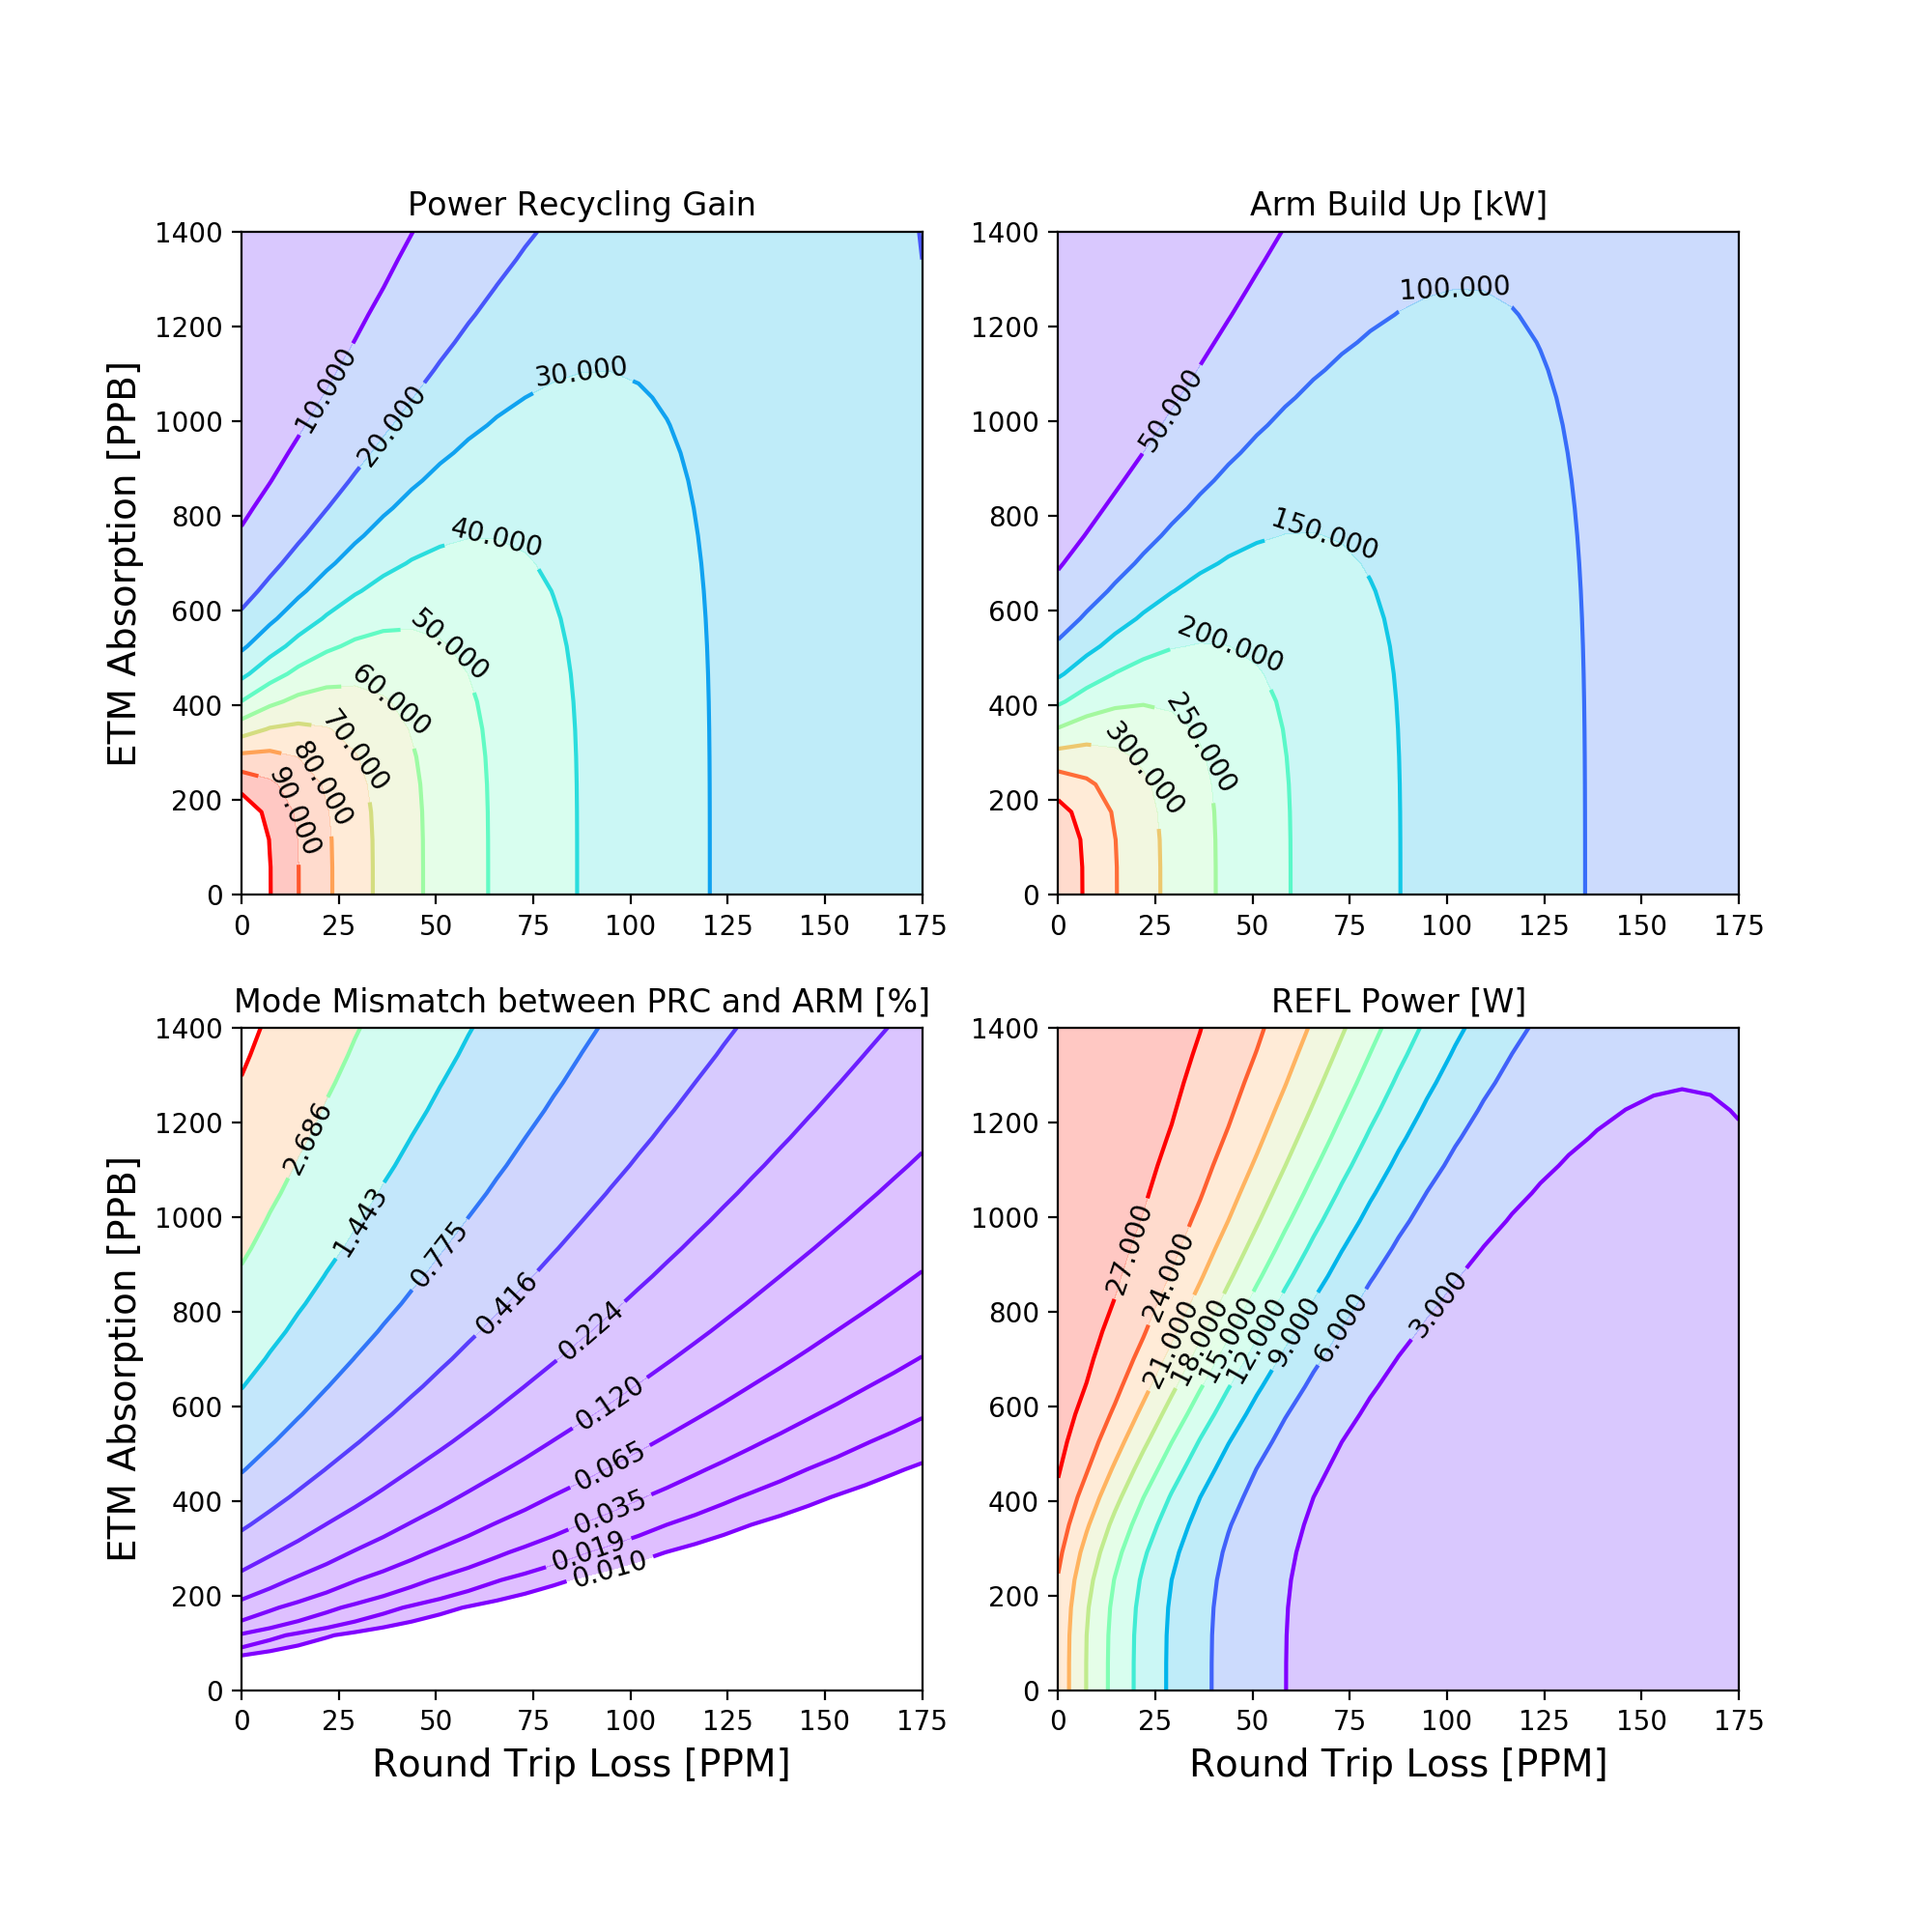
\includegraphics[height=0.5 \textheight]{../Figures/Simplified_PRC_ARM_etm_abs.png}
		\end{minipage}\hfill
		\begin{minipage}{0.5\textheight}
			\centering
			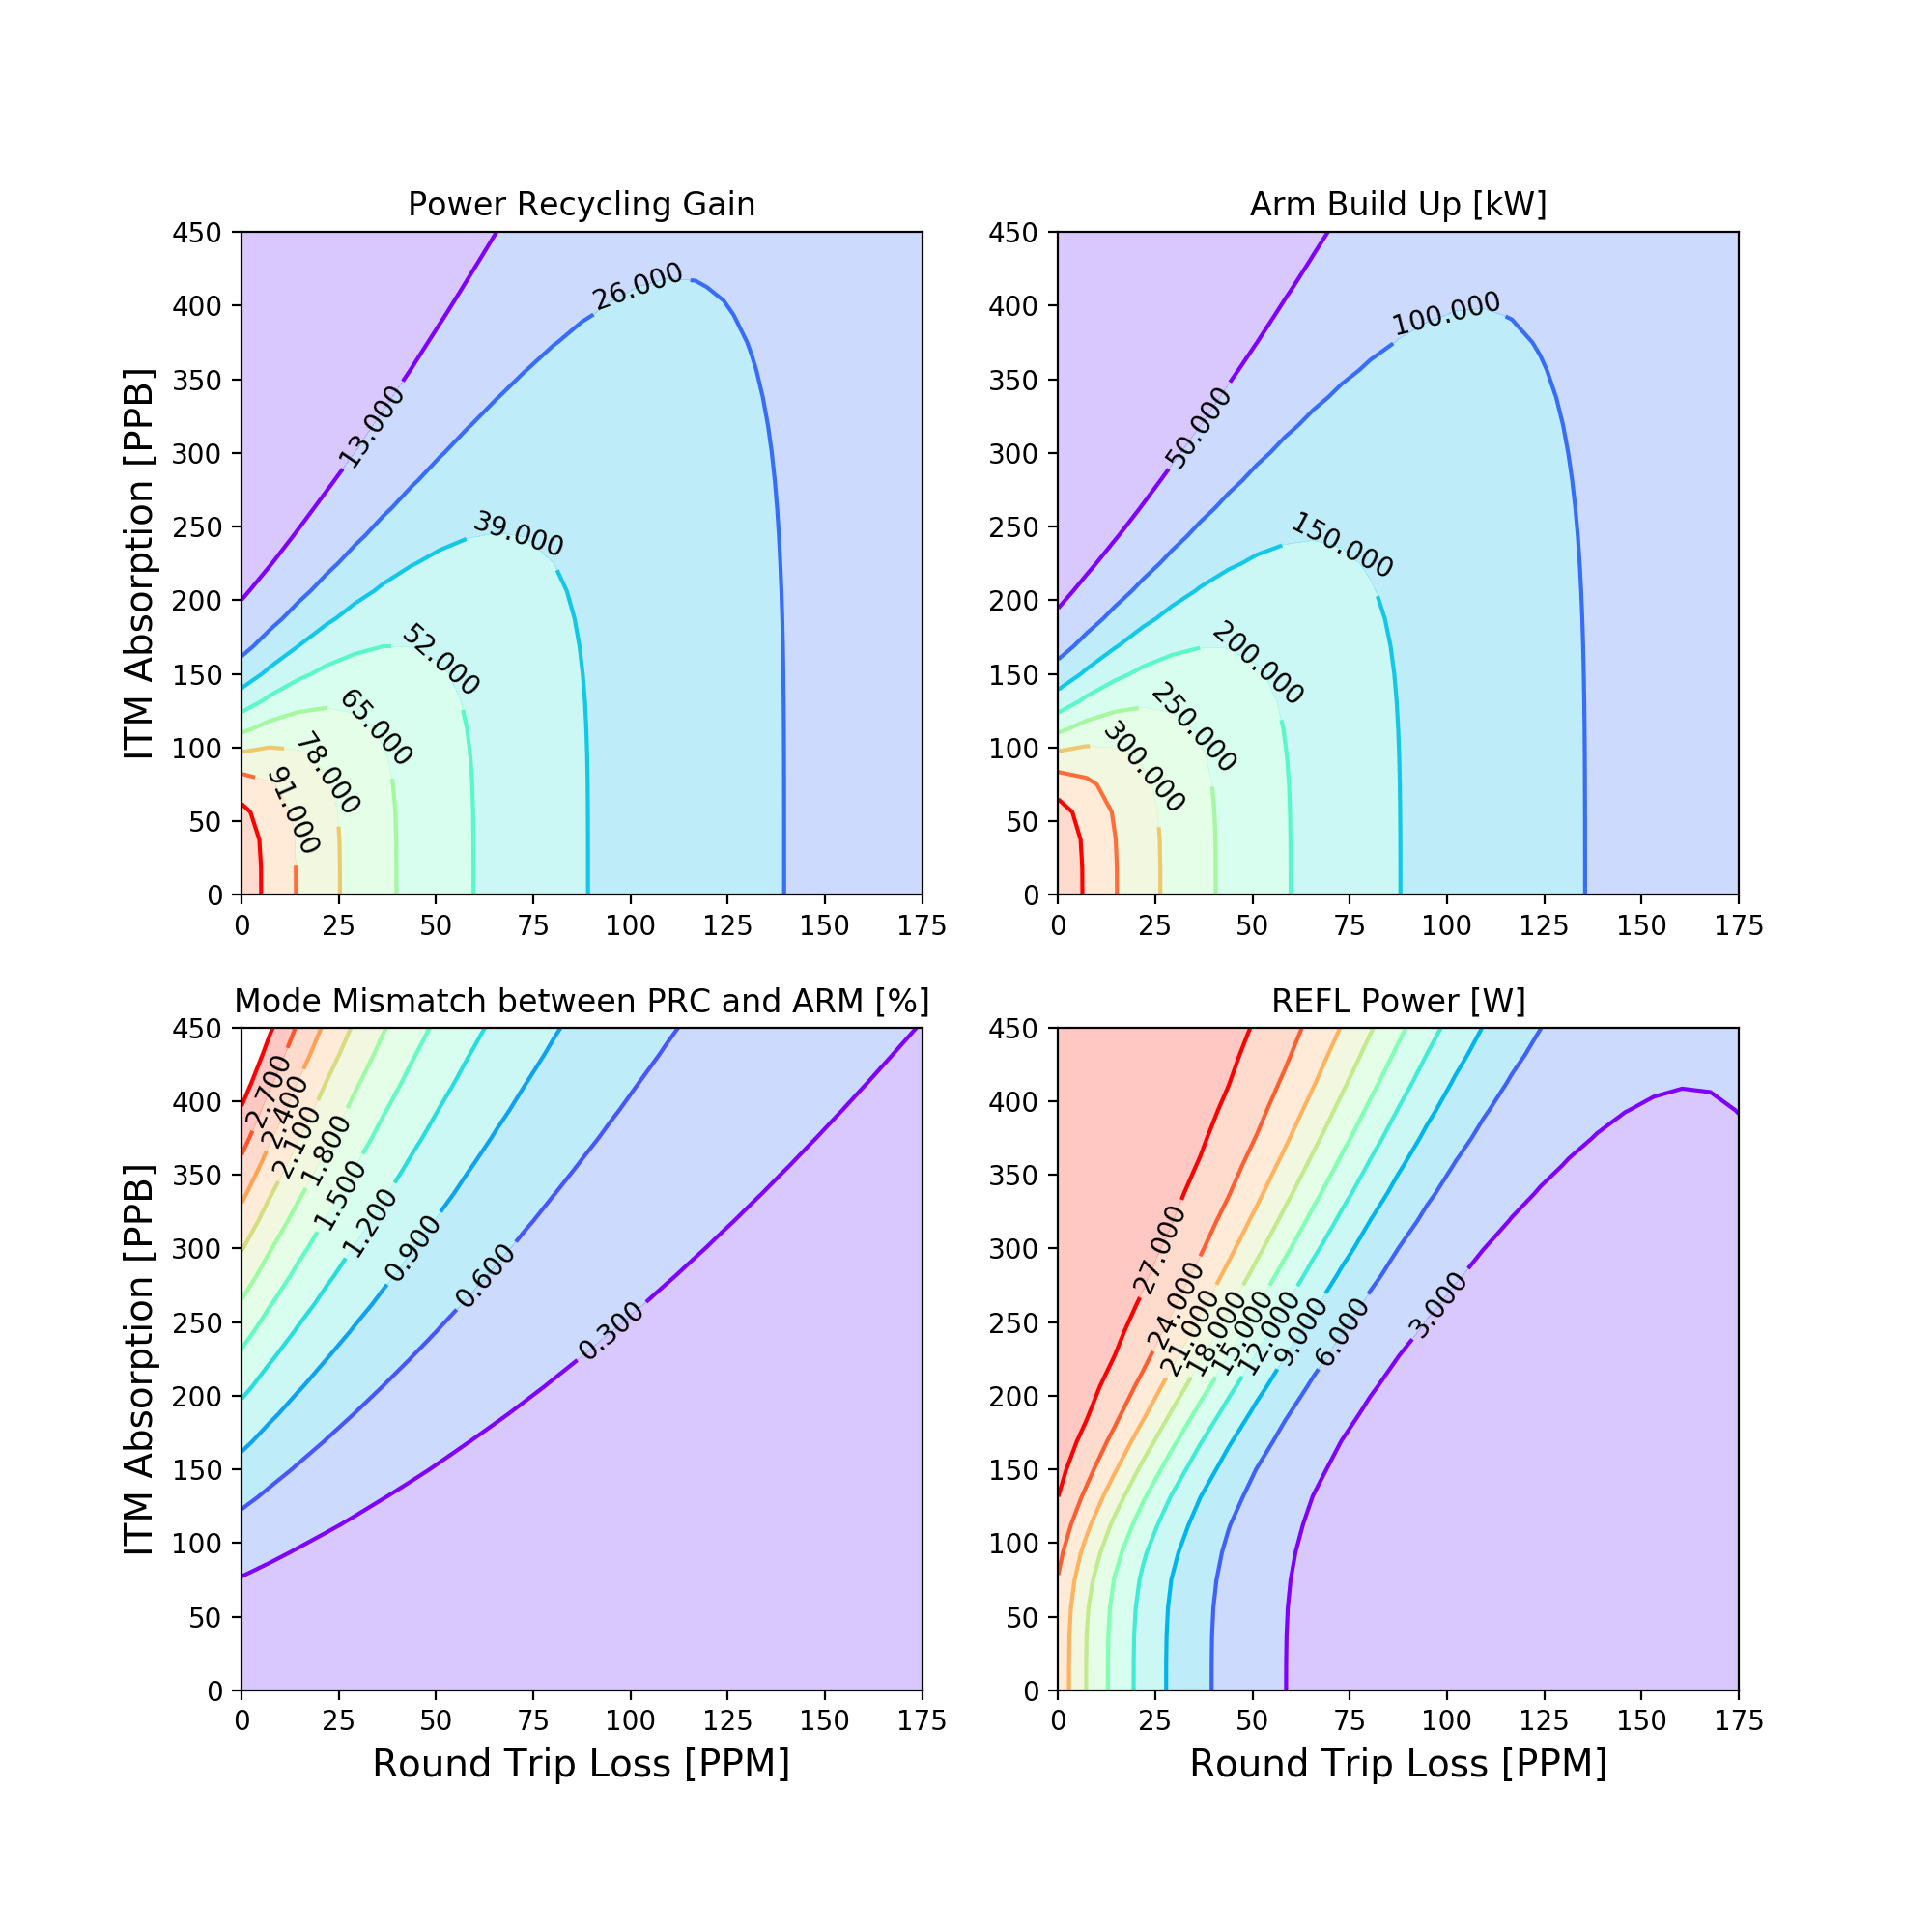
\includegraphics[height=0.5 \textheight]{../Figures/Simplified_PRC_ARM_itm_abs.png}
		\end{minipage}
		\caption[Interferometer DC powers as a function of round trip arm loss and test mass absorption.]  
		{\textbf{Interferometer DC powers as a function of round trip arm loss and test mass absorption.}
			Simplifying the power recycling cavity and a combined arm model to understand the powers as a function of loss has a few advantages with regards to computational time and the results are easier to conceptually understand.  Here, absorption changes the radius of curvature and substrate thermal lens which results in some mode mismatch while the round trip loss takes into account the rest of the higher order modes from point absorbers.  The ITM absorption has a much larger effect on the overall power recycling gain loss by almost a factor of 3 compared to ETM absorption.  Of course, the simplified model will fall short in describing effects on the antisymmetric signals of the full interferometer.
		}
		\label{fig:simple_prc_arm}
	\end{sidewaysfigure}

\clearpage

\section{Higher Power Operation}
	The goal for O3 is 150 kW of circulating power in the arms. With the sensors and tests described in the preceding sections, a cohesive plan to pre-load the interferometer was implemented in order to achieve stable higher power operation in the detectors.  Generally, the Thermal Compensation System has two goals: Firstly, the actuators are used to pre-load the test masses with heat in anticipation of the lensing due to the interferometer while operating at full lock and higher power.  Secondly, the amount of mode-matching between the coupled cavities must be optimized in order to achieve the best sensitivity.  Using the absorptions measured in Figure \ref{fig:hws_abs}, it is possible to estimate the total amount of lensing from self-heating as a function of input power (see Figure \ref{fig:TCS_ITMs}).

	In principle, the Hartmann measurements of absorbed power should provide sufficient information to pre-loaded the interferometer in anticipation for 50 Watts of input power.  The biggest difficulty associated with implementing this thermal compensation scheme was consistently locking DRMI in high micro-seismic conditions. This could be contributed to misalignment of CO2 lasers to the test masses, which were initially aligned using the Hartmann sensors and double-checked by cycling the lasers on/off to measure the single bounce interferometer beam deflection at the anti-symmetric port. At Hanford, this difficulty for reliably locking the interferometer forced a reduction in pre-loading, so with the combination of estimates provided by the Hartmann Sensors and experimentation with the CO2 power levels at each stage of increasing the PSL power, the interferometer is able to consistently lock at 30 Watts of PSL input power and $\approx 140 \; kW$ of circulating arm power. 
	
	\begin{figure}[t!]
	\centering
	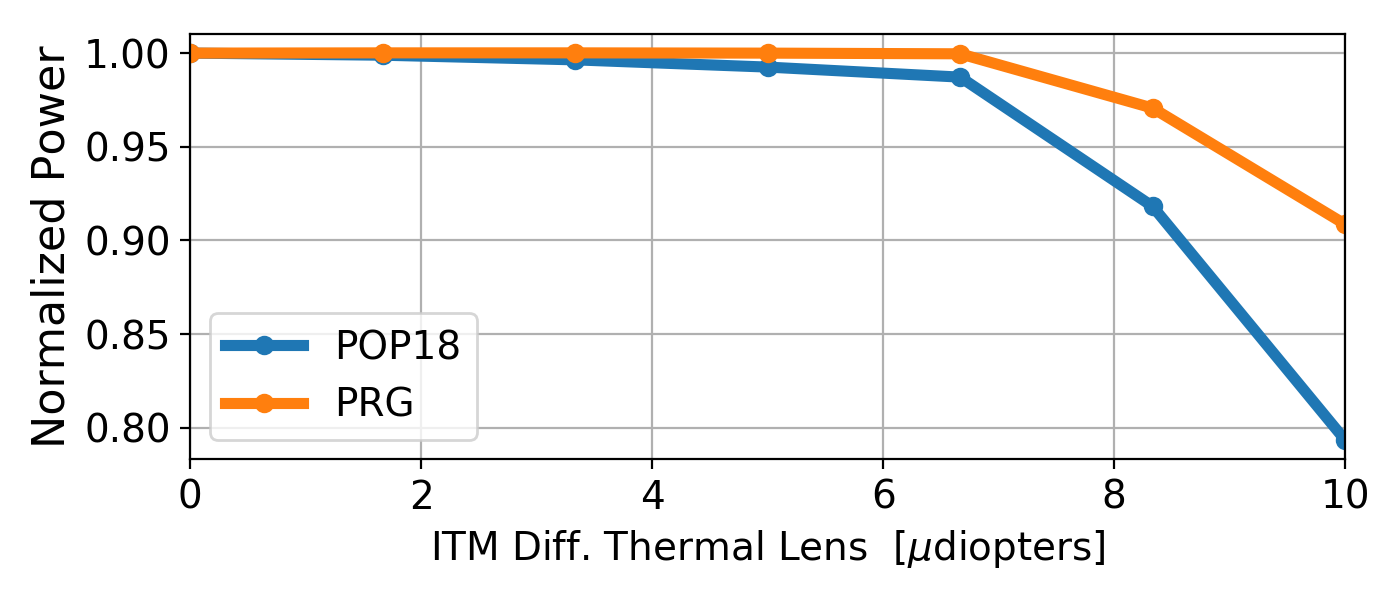
\includegraphics[width=0.75 \textwidth]{../Figures/POP_18dive.png}
	\caption[Model of POP-18 as a function of differential thermal lensing using FINESSE.]  
	{\textbf{Model of POP-18 as a function of differential thermal lensing using FINESSE.}
		The horizontal axis is differential lensing between the ITMX/ITMY substrates and the vertical axis represents the normalized power when locked with nominal mode matching.  Even with modest differential lensing (10 microdiopters), the buildup drops by 20 percent and eventually the simulation has trouble maintaining resonance, similar to the actual interferometer.
	}
	\label{fig:POP18}
	\end{figure}

	During the early phases of commissioning for higher power at Hanford, most of the lock losses occurred when the 18 Mhz sidebands in transmission of PR2 (POP-18) would fall below a certain threshold level of approximately 70\% of buildup compared to locking at 2 Watts of input power.  This effect was not observed at Livingston and can be attributed to the point absorber that uniquely contaminated H1-ITMY.  To study the effects of differential uniform lensing in an interferometer, FINESSE is able to simulate the POP-18 signal at the power recycling pick-off port demodulated at 18 MHz which shows the sideband power buildup in the power recycling cavity (see Figure \ref{fig:POP18}). In this particular simulation the differential lensing requires finding a new operational point to continually lock the longitudinal degrees of freedom.  Additionally, the simulated sensors which are used to maintain resonance and measure the RF power need to be re-phased; this agrees with the analytical calculation mentioned in Section \ref{Sec:TL_lensing} where the carrier power recycling gain is not as adversely affected by the substrate thermal lens compared to the sideband fields.
	
	In the ideal mode matching scenario, the carrier and sidebands resonate differently in the power recycling cavity; where the 9 Mhz modulation sidebands has approximately a factor of 10 larger finesse than the carrier \cite{kiwamu_freq1}.  However, this assumes a lossless interferometer and needs to be revisited in the presence of substrate thermal lensing.   As with all Pound-Drever-Hall locking, an error signal relies on the static and varying field accumulating different phases to lock the cavity. As lensing causes more losses for the sideband compared to the carrier, the difference in accumulated phase between the two fields is reduced hence the optical gain starts to diminish.  For the current Advanced LIGO configuration, all vertex degrees of freedom (PRCL, SRCL, MICH) utilize the POP port for their error signals shown in Figure \ref{fig:vertex_OLTF}. The degradation can be estimated by injecting a dither line into each degree of freedom and digitally demodulating the respective sensors at the excitation frequency, see Figure \ref{fig:POP18_POP90}.  This provides insight on how much the optical gain/phase shifts as a function of heating.  When powering up to 30 Watts, the loss of optical gain in PRCL is almost 80\% with a 10 degrees phase shift, which enough to drive the system towards an unstable loop.  This can be compensated by adjusting the digital gain but that fix is only temporary because the problem stems from an optical loss so eventually, the error signal will have no linearity about the zero-point.  Alternatively, searching for optimal thermal compensations settings to re-gain theses losses can be very time consuming because of the long thermal time constants and in the case of point absorbers, the current thermal compensation system is not designed to correct the high spatial frequencies.  As previously mentioned, one of the main limiters to higher power operation will be reducing the optical loss from mode mismatch.

	\begin{figure}[t!]
		\centering
		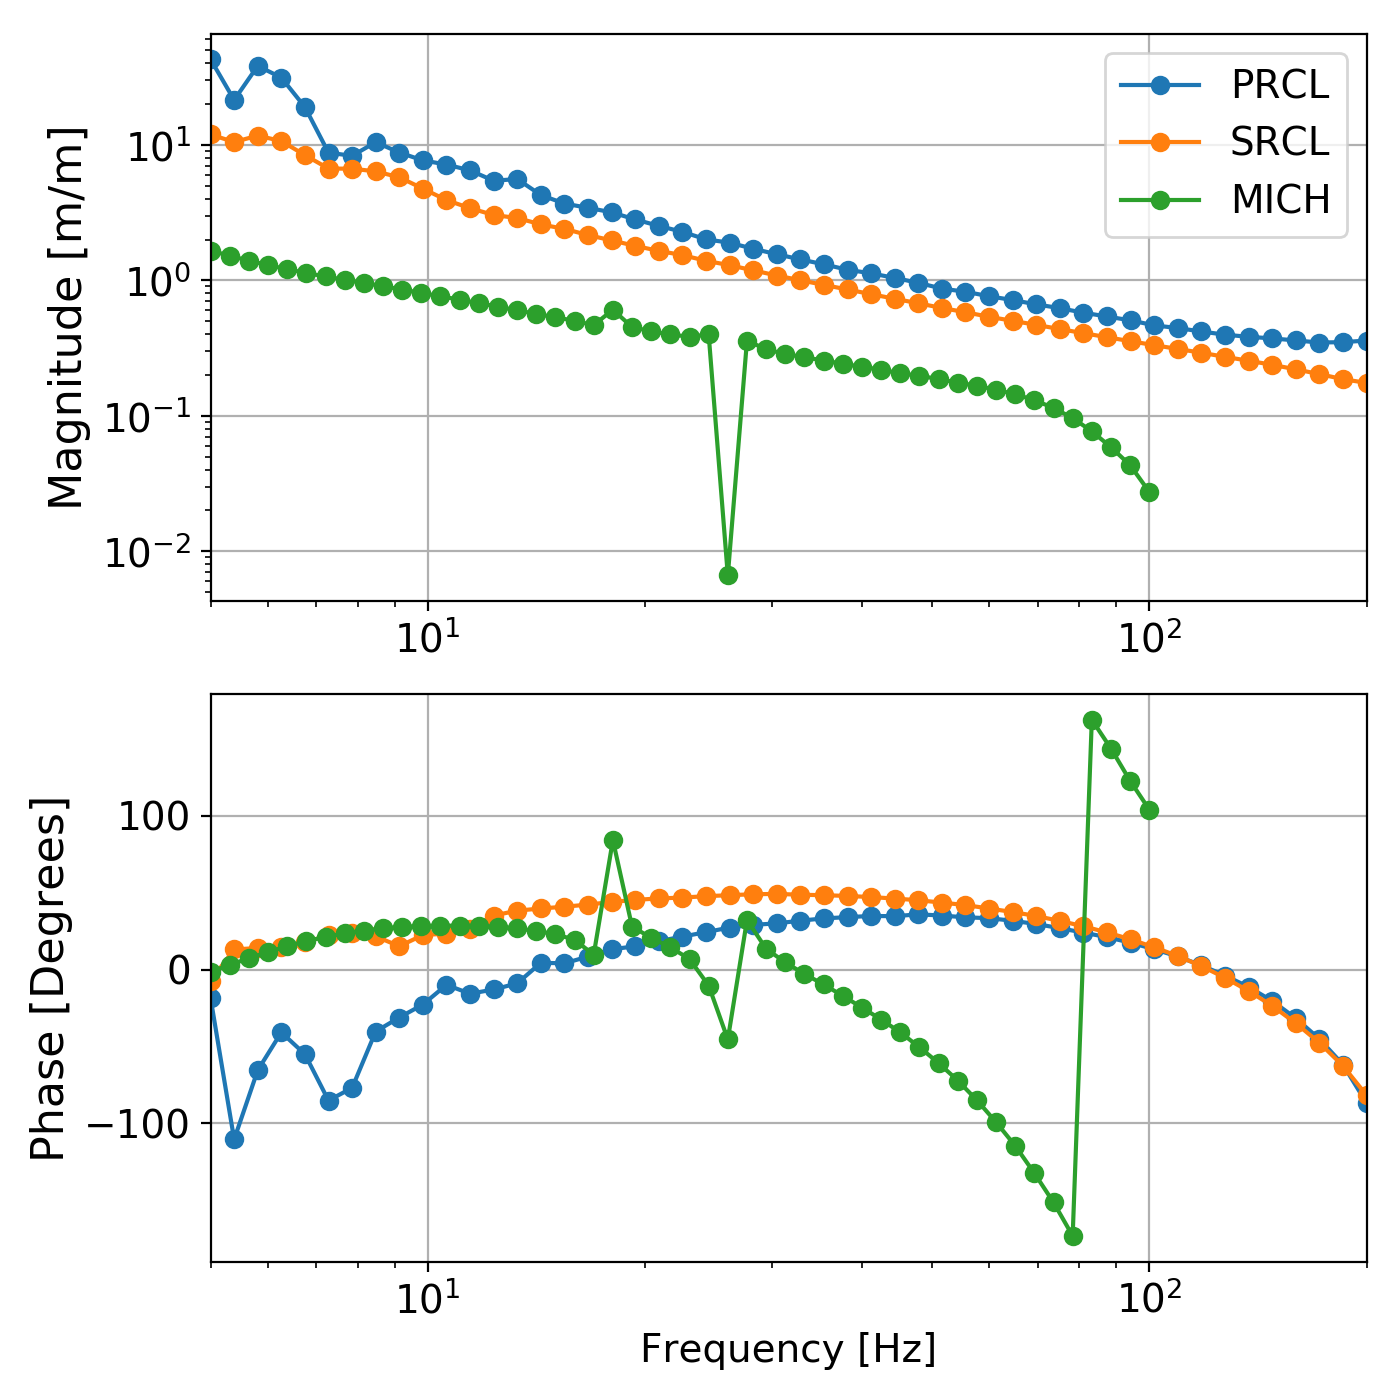
\includegraphics[width=0.75 \textwidth]{../Figures/MeasuredVertexOLF.png}
		\caption[Vertex open loop transfer functions while in Nominal Low Noise.]  
		{\textbf{Vertex open loop transfer functions while in Nominal Low Noise.}
			The nominal UGF for PRCL is around 45 Hz.
		}
		\label{fig:vertex_OLTF}
	\end{figure}
	
	\begin{figure}[t!]
		\centering
		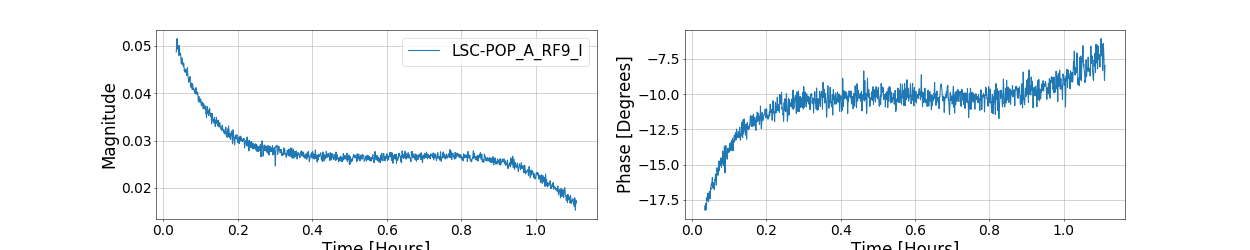
\includegraphics[width=1.0 \textwidth]{../Figures/PRCL_EXC_LSC-POP_A_RF9_I.png}
		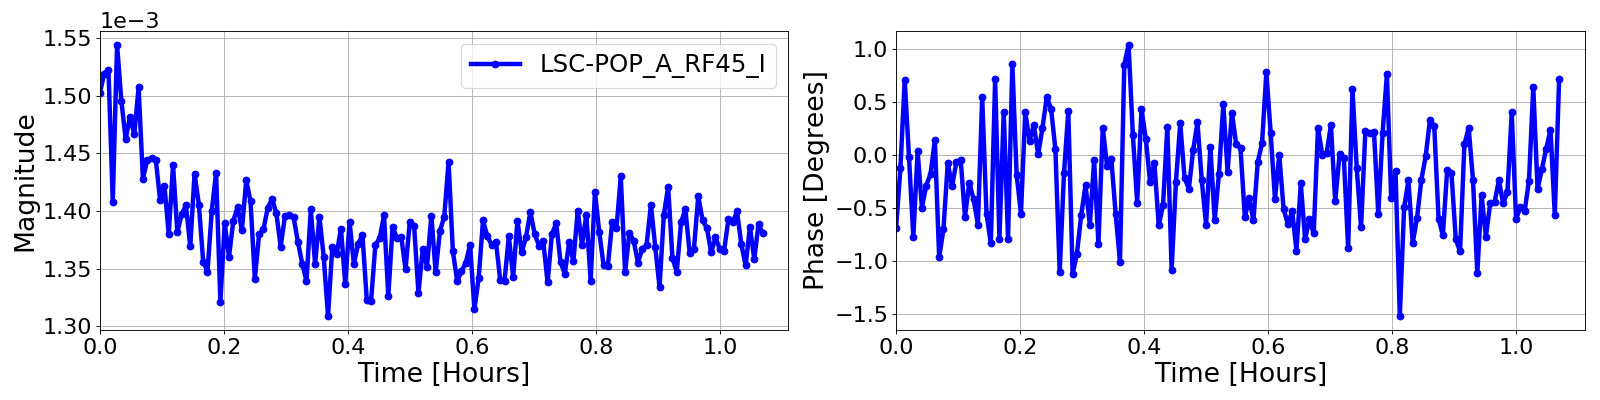
\includegraphics[width=1.0 \textwidth]{../Figures/SRCL_EXC_LSC-POP_A_RF45_I.png}
		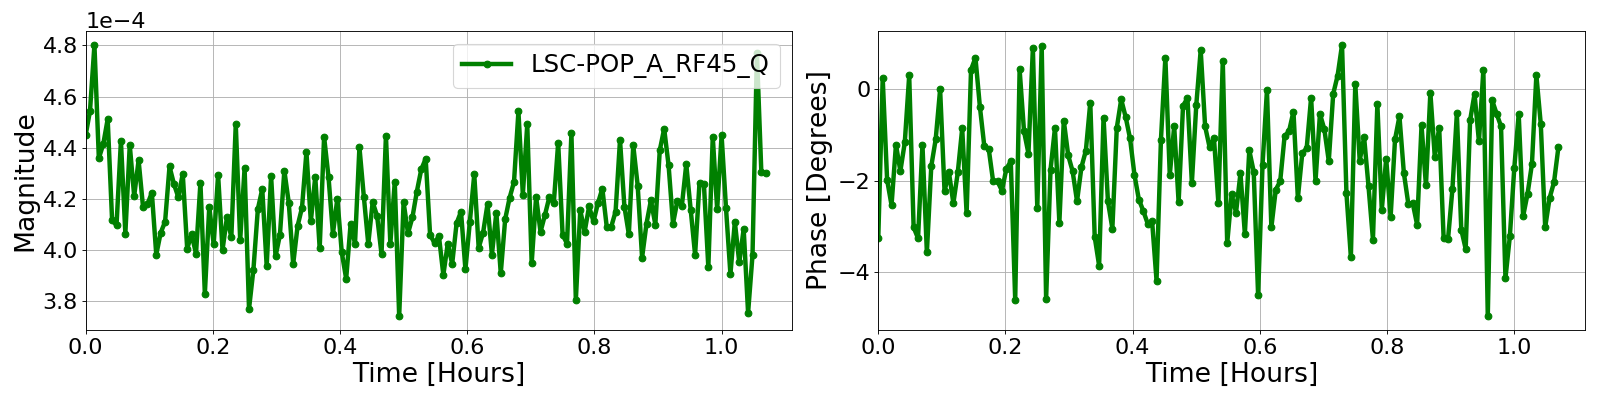
\includegraphics[width=1.0 \textwidth]{../Figures/MICH_EXC_LSC-POP_A_RF45_Q.png}
		\caption[Measuring vertex optical gains as a function of heating.]  
		{\textbf{Measuring vertex optical gains as a function of heating.}
		At time t=0, the power begins increasing from 2 watts of input power to 20 watts. In PRCL, there is a reduction to 80\% of the starting magnitude and 7.5 degrees of phase rotation with the first power increase. At 0.9 hours, the input power goes from 20 to 30 watts and the magnitude drops to about 30\% of the original gain which results in a lock loss.  As for the SRCL and MICH degrees of freedom, there are slight changes first power increase but not nearly as bad as PRCL.
		}
		\label{fig:POP18_POP90}
	\end{figure}

\clearpage

\section{Mode Matching from the OPO to the OMC}
	Mentioned in Chapter 2, one of the main limitations to effective squeezing is mode mismatch which needs to be characterized carefully.  Generally, the mode exiting the OPO and OMC cavities are accurately determined from design values but the path lengths and mode profile was measured and the results are presented in this section.
	
	\begin{figure}[]
	\centering
	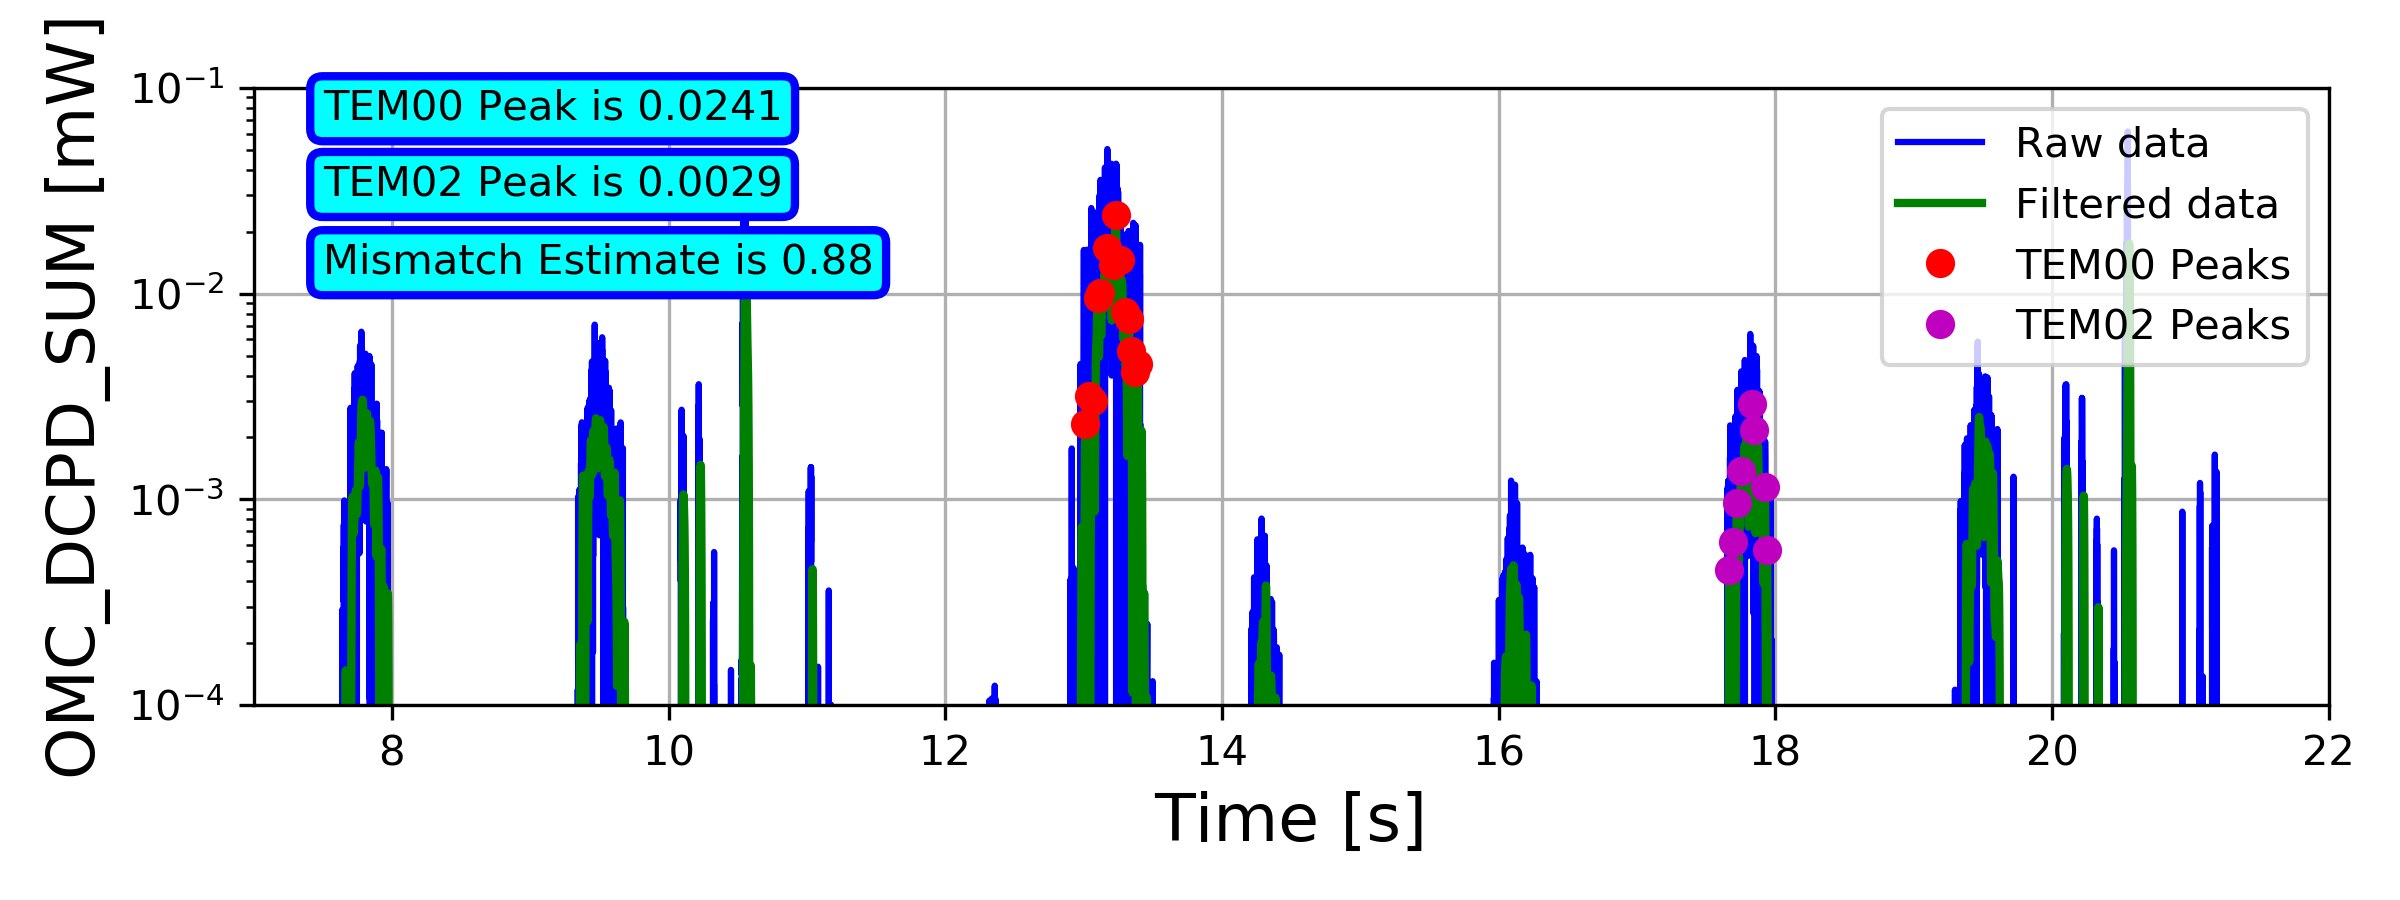
\includegraphics[width=0.7\textwidth]{../Figures/Lens_Closest_to_OPO.png}
	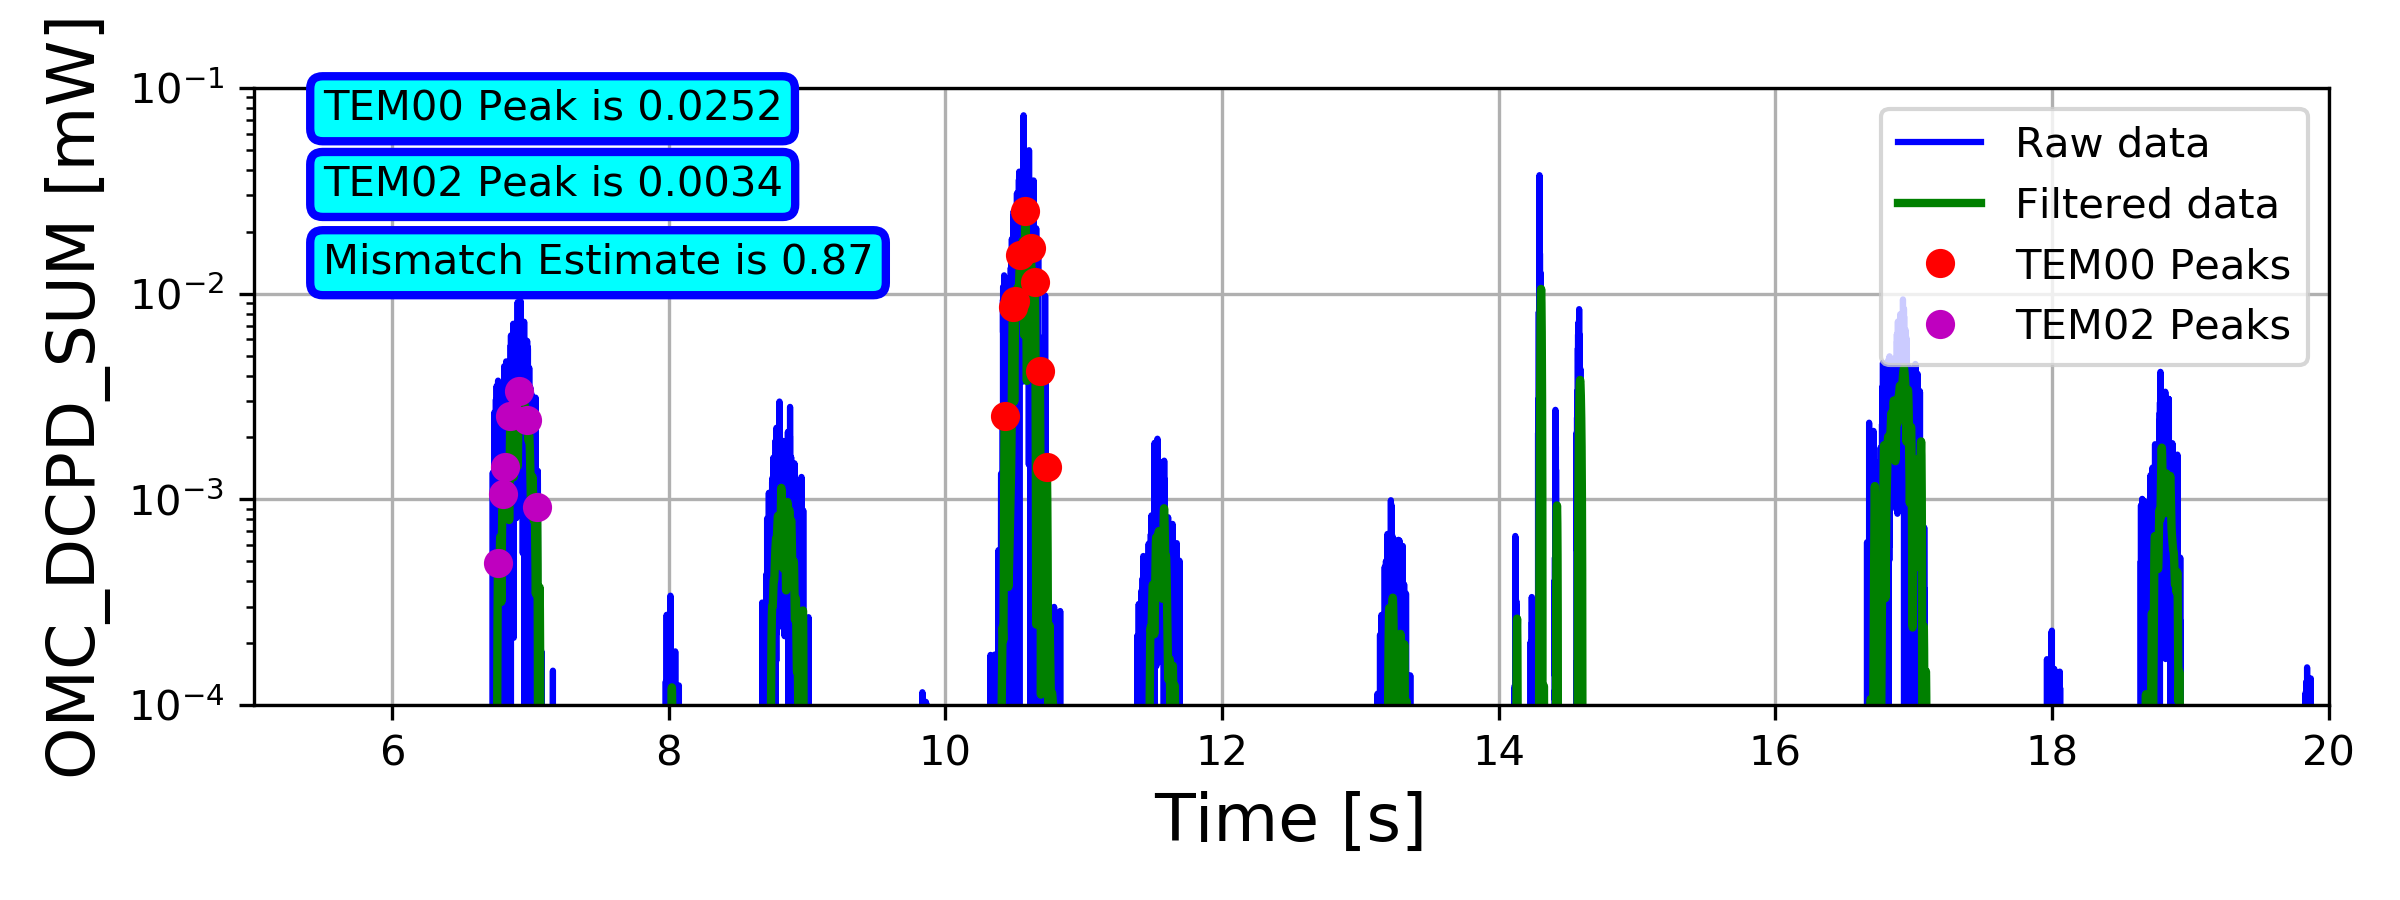
\includegraphics[width=0.7\textwidth]{../Figures/Lens_in_Center_Position.png}
	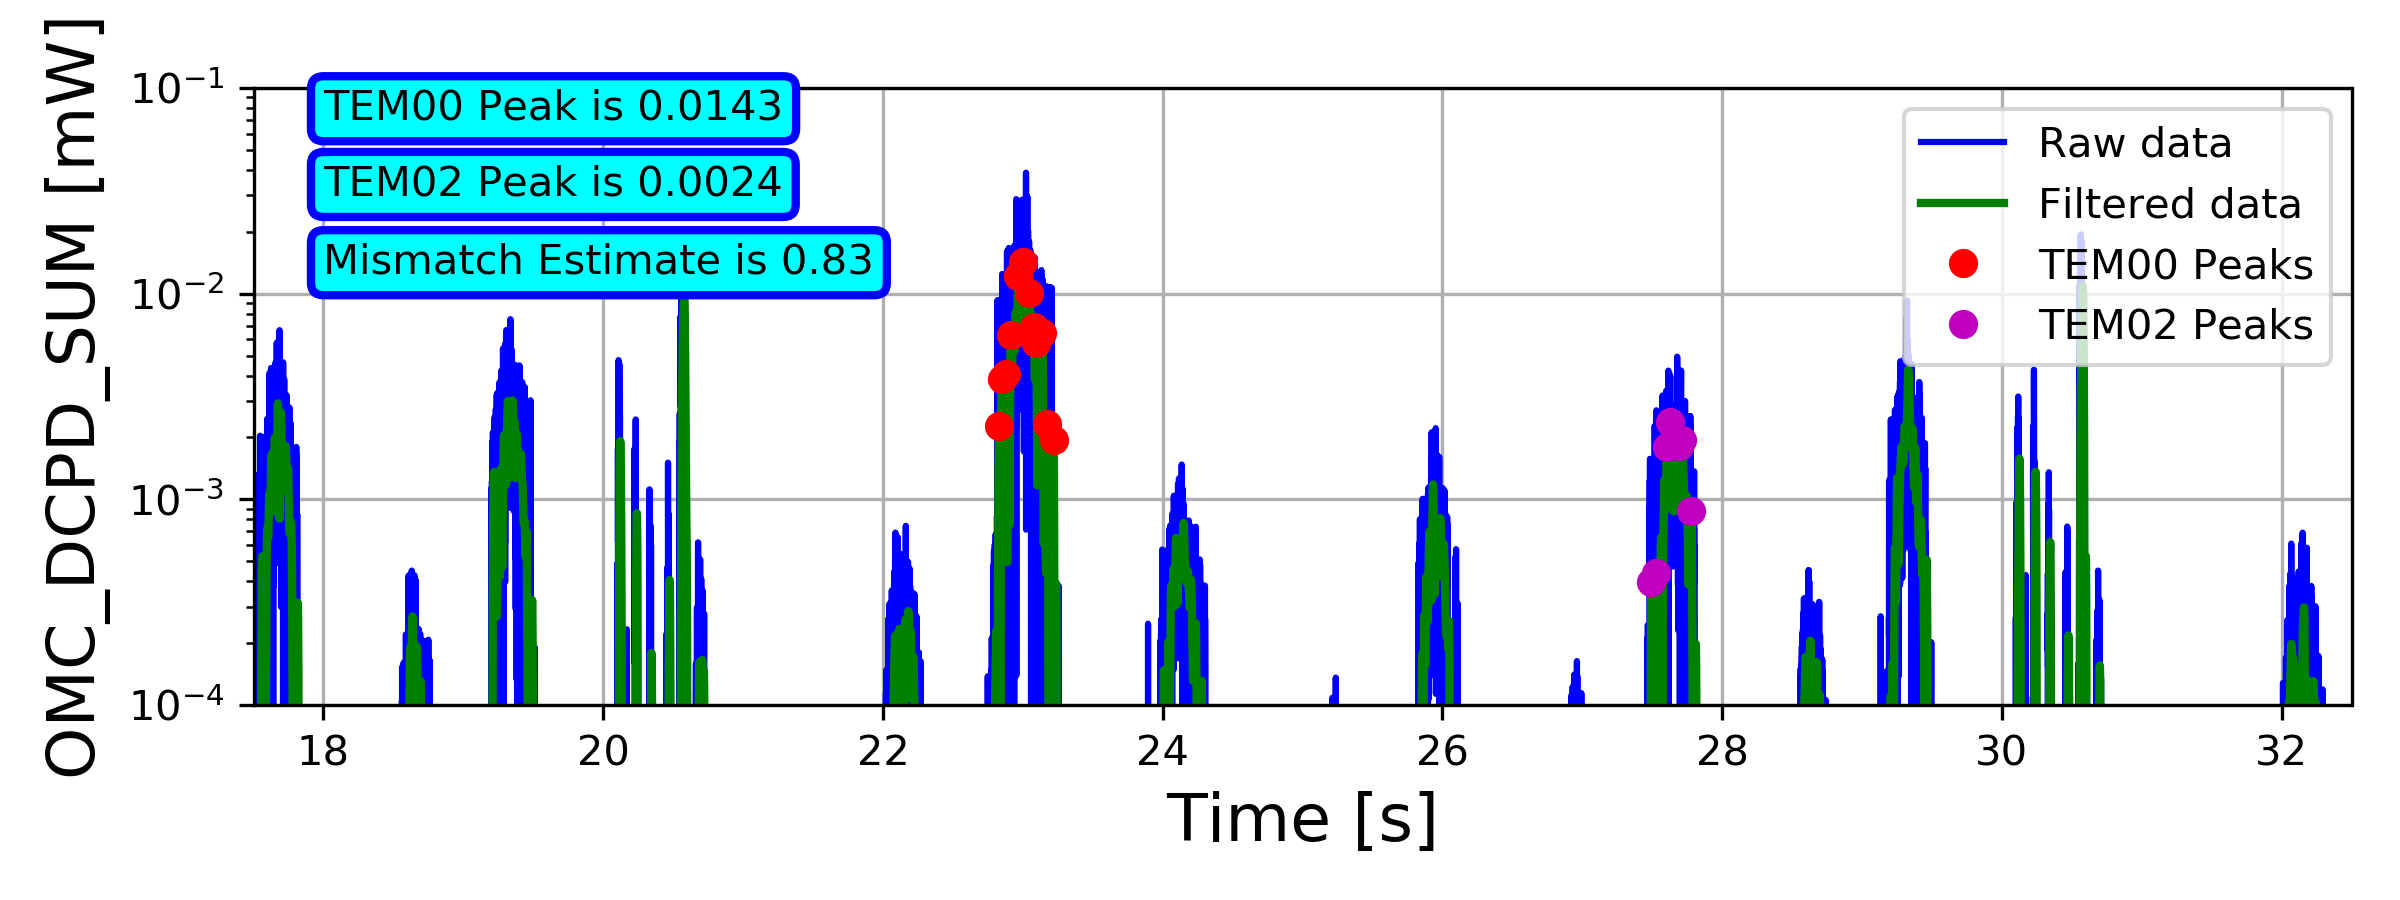
\includegraphics[width=0.7\textwidth]{../Figures/Lens_Furthest_from_OPO.png}
	\caption[OPO to OMC cavity scanning for various Lens2 positions.]  
	{\textbf{OPO to OMC cavity scanning for various Lens2 positions.}  The top figure has the lens closest to the OPO along the propagation axis, the middle figure represents Lens2 at half the actuation range and the bottom figure shows the lens furthest from the OPO.  During this time, the OMC ASC control loops were closed on the reflected QPDs to minimize the odd order mode coupling.  
	}
	\label{fig:OPO_to_OMC_scan}
	\end{figure}

	Using the OMC as an optical spectrum analyzer is one simplest methods for understanding the mode matching coming out of the interferometer.  In a single bounce configuration, measuring the ratio between the second order mode and the fundamental gives a first look at the limit of matching.  Similar techniques can be used with the squeezed beam as well and during commissioning of the squeezer, a mode mismatch between 12-17\% was observed which led to a re-design of the OPO to OMC optical path.  Figure \ref{fig:OPO_to_OMC_scan} shows the results for scanning the OMC length using PZT2 with the  ASC control loops closed on the reflected QPDs to minimize odd-order mode coupling.  The measurements were taken in-air which made the results rather noisy so before the peak-finding algorithm tries to fit the 00 or 02 modes, the data is low-passed with a corner frequency of 1kHz.
	
	Using a well-calibrated mode profiler that measures beam sizes along the propagation axis is the most direct way of determining OPO to OMC mode matching.  This method can also predict the actuator Gouy phase of the second lens after the OPO, which is on a translation stage with approximately 4 centimeters of range. Generally, the length measurement between optics is the largest systematic error especially in the near-field where beam sizes do not change very much as a function of $\hat{z}$.  In addition, places to put a beam profile become very limited as HAM6 becomes crowded with optical components.  In preparation for squeezing in Advanced LIGO, the mode matching from the OPO to OMC was measured and found to be approximately 88\% at best. When implementing a telescope with fast lenses, the distances between optics must be stringently characterized but the OPO platform is very crowded along the output path so it was very difficult to accurately measure the path lengths with a ruler.  Between the second lens and ZM1, the table is much clearer and by removing Lens2, the Gouy phase is approximately in the far-field which means the distance measurements can be more easily measured as a function of beam size.  Figure \ref{fig:OPO_to_ZM2} shows the results of characterizing the OPO output mode as it enters HAM5 by removing Lens2, a fit constrains the Lens1 positioning and the OPO mode is assumed from its design document \cite{Oelker_FD_sqz}.
	
	With the poor mode matching shown in Figure \ref{fig:OPO_to_OMC_Old}, the fast telescope lenses needed to be replaced, or otherwise, risk being the limit to effective squeezing for O3.  The available range in the translation stage did not allow for increased matching and the crowded OPO platform did not permit coarse moves of Lens1. In addition, moving the translation stages for Lens2 closer to the OPO cavity does not gain any extra mode overlap.  The next option was replacing the lenses with a solution which did not incorporate large actuation range but was more suited for mode matching.  There were a few clean lenses available that provided the right solution but greatly reduced the translation stage efficacy, on the other hand, this made the telescope placement much more robust to path length errors which is the original problem to begin with.  The new model is shown in Figure \ref{fig:OPO_to_OMC_New} where the lenses are now  $f^{\text{new}}_{\text{Lens1}} = 250$ mm and $f^{\text{new}}_{\text{Lens2}} = 350$ mm where Lens1 is closer to the OPO output.   The calculated overlap integral between the expected OMC mode and the squeezer is on the order of 99\% with very little sensitivity in the Lens2 positioning as expected.  Follow up measurements with OMC scans in-vacuum indicate approximately 95\% mode matching between the OPO to SRM and back to the OMC, this is due to the astigmatism mentioned previously that is still prevalent after changing the lenses.  However, the mode matching from the OPO to ITMs and back to the OMC shows 99\% mode matching with the new lens configuration \cite{modematch99} which is effectively the path of squeezed light.  It is important to note that measurements taken in-vacuum had pre-loaded TCS settings in anticipation for 50 Watts.
	
	For future implementations of high sensitivity telescopes, length measurements between optics will need to be more stringently constrained with specialized tools such as laser range finders or mechanical jigs while simultaneously re-confirmed with profile scans to understand the laser beam entering the interferometer.  Distances between optics were the largest source of uncertainties in these measurements so understanding the optical path length will help curb the systematic errors.
	
	\begin{figure}[]
		\centering
		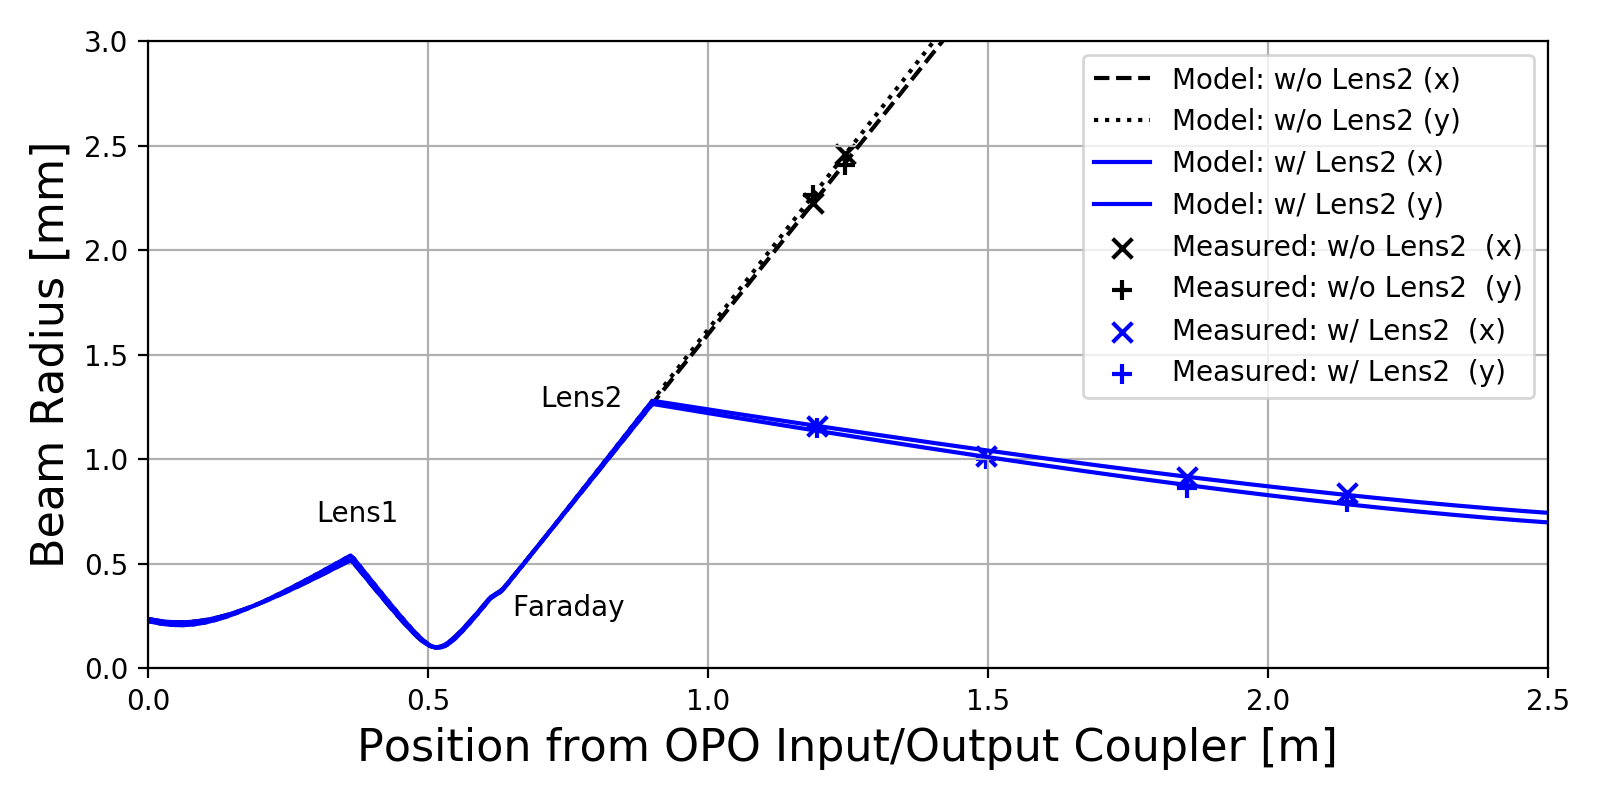
\includegraphics[width=0.8 \textwidth]{../Figures/OPO_to_ZM2_fit.png}
		\caption[Mode measurement from the OPO.]  
		{\textbf{Mode measurement from the OPO.}
			The results without Lens2 are shown in black for two transverse directions (x/y) and constrain the distance of Lens1 relative to the OPO output.  Then, Lens2 is replaced back in its original position on a translation stage at half the range and measurements were taken in order to constrain the distance between Lens1 and Lens2.  The beam sizes were fit to find the Gaussian q-parameter entering HAM5. There is some slight deviation in the transverse directions after Lens2, possibly from misalignment of the lens.  This method seems to provide a good model of what beam is being injected from the squeezer side.
		}
		\label{fig:OPO_to_ZM2}
	\end{figure}
	\begin{figure}[t!]
	\centering
	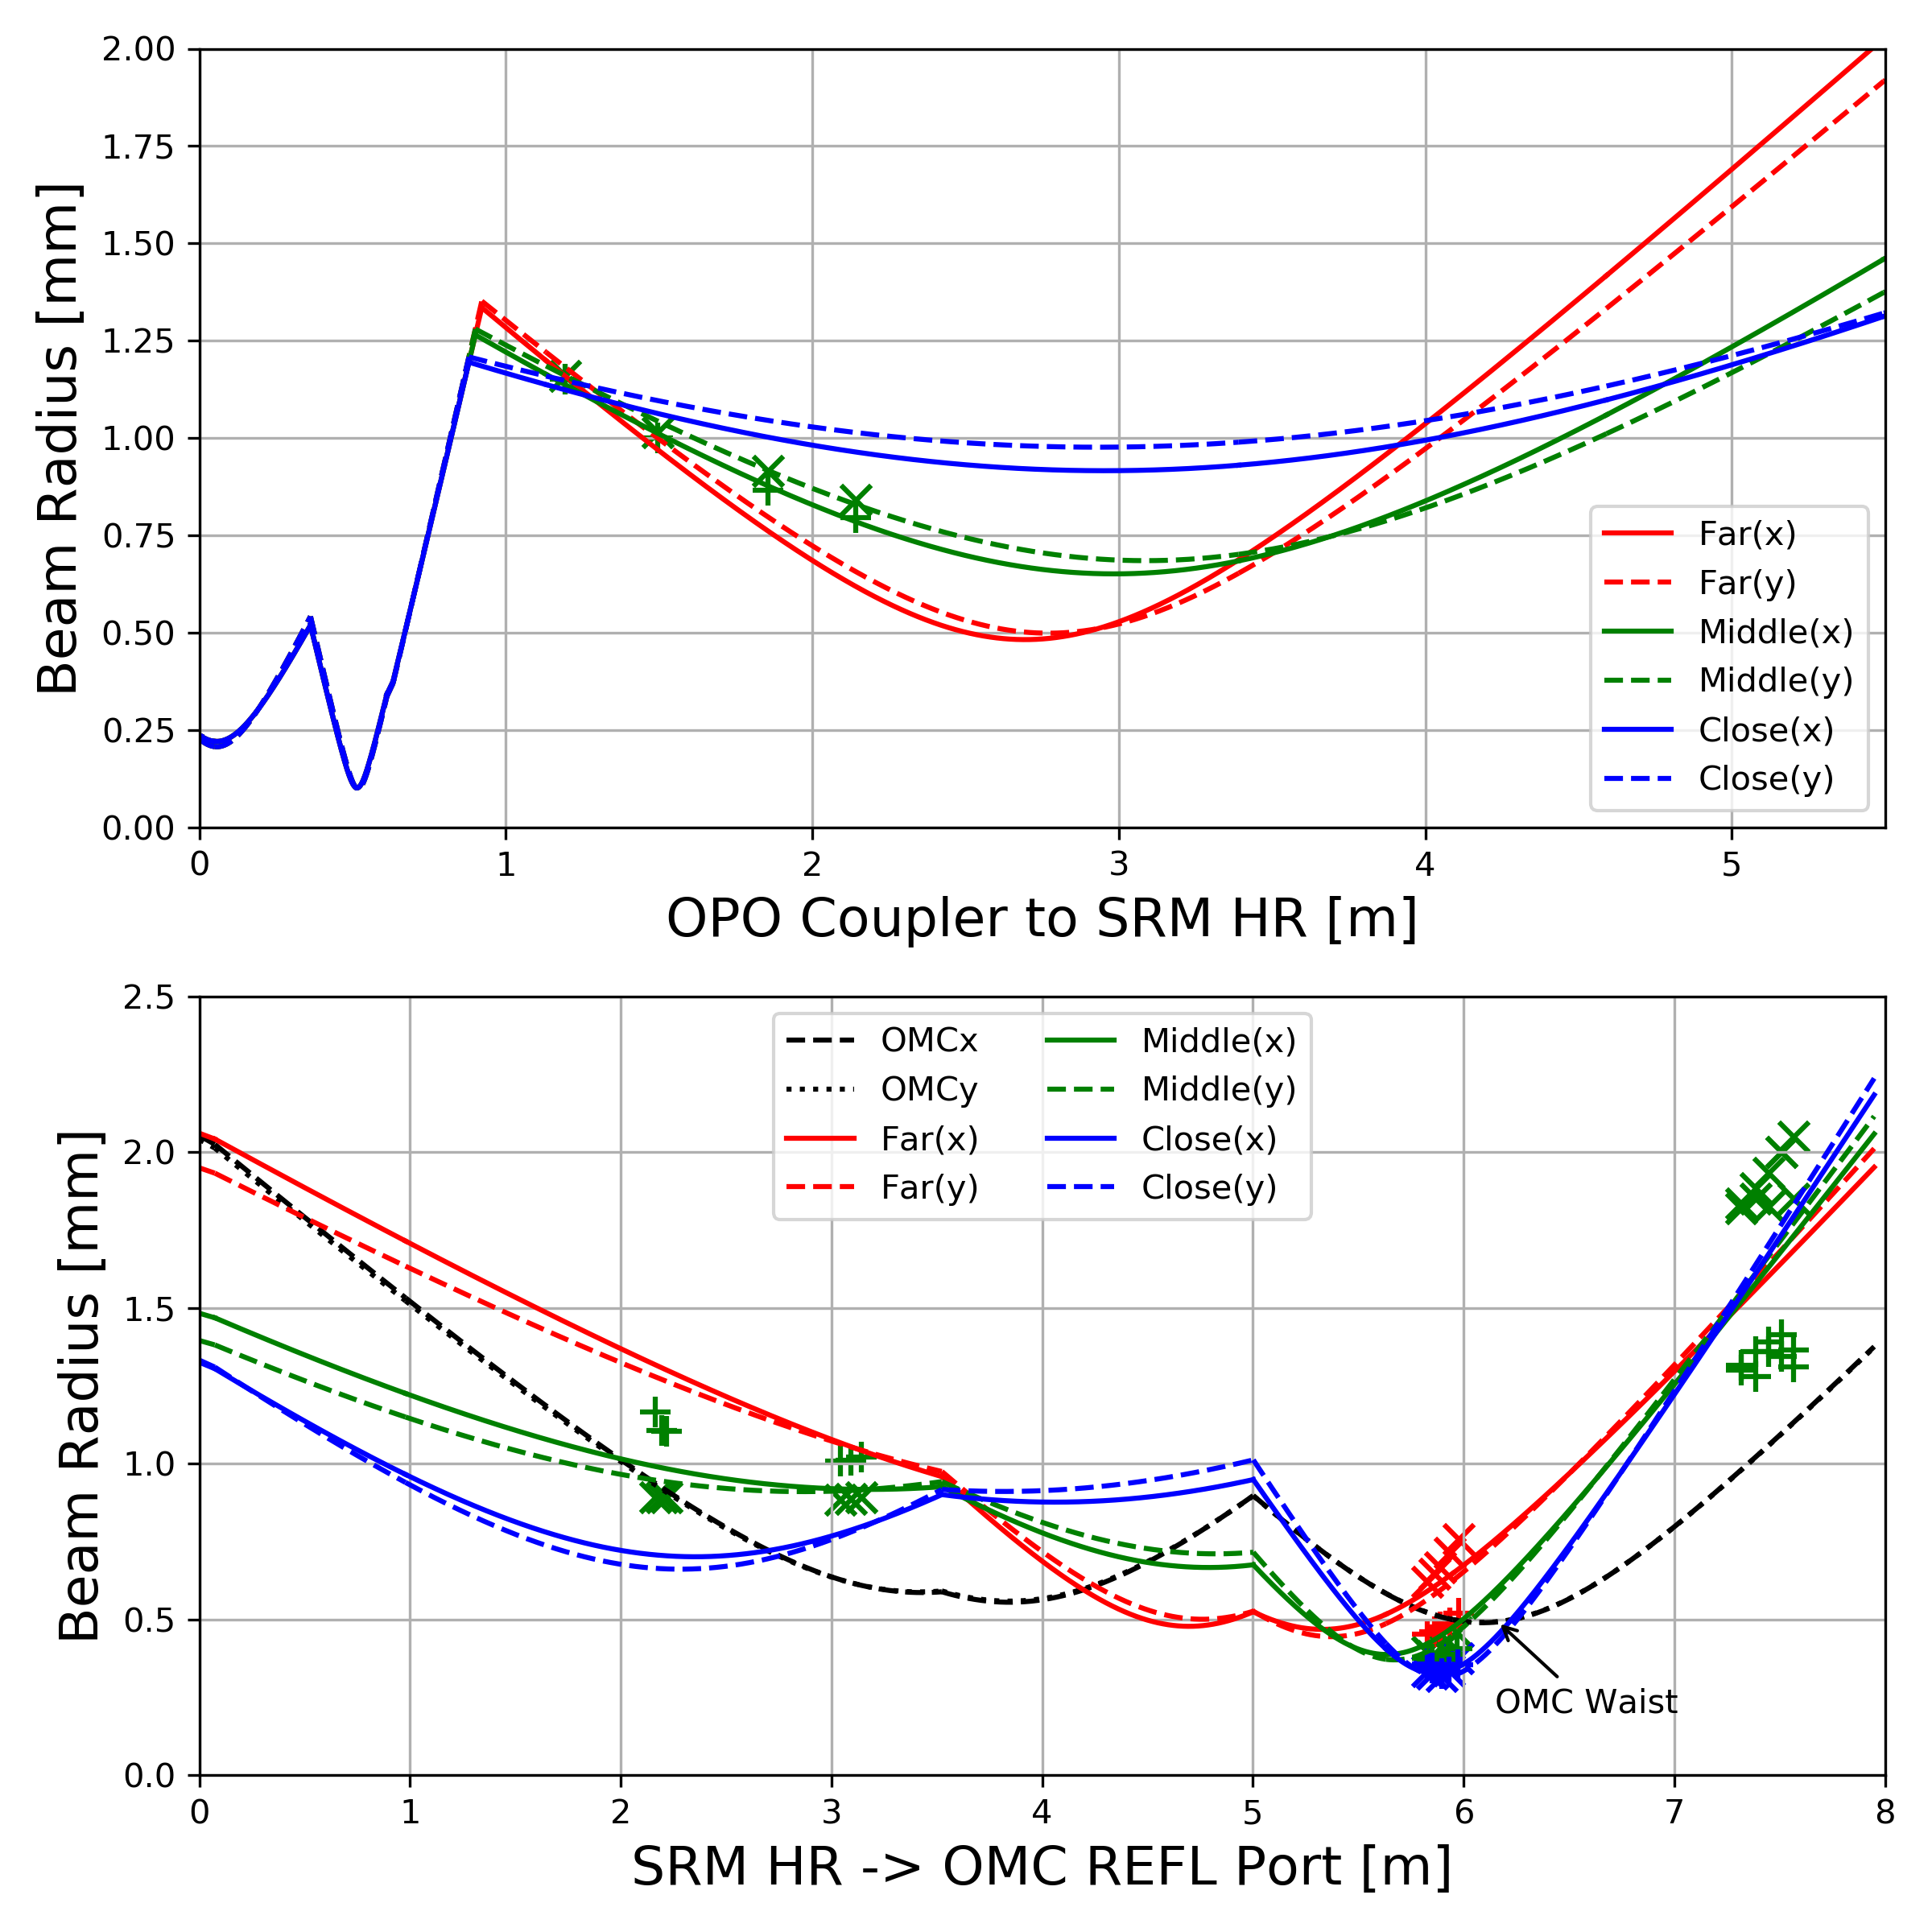
\includegraphics[width=0.8 \textwidth]{../Figures/OPO_to_OMCREFL_Oldlenses.png}
	\caption[Projecting the modes from the squeezer to the OMC.]  
	{\textbf{Projecting the modes from the squeezer to the OMC.}
		Determining the actuation range with the translation stage using the as-installed focal lengths, $f_{\text{Lens1}} = 111$ mm and $f_{\text{Lens2}} = 334$ mm, showed that the mode matching into the OMC was at most 80\% with various translation stage positions with "Close" referring to the position of Lens2 relative to the OPO cavity.  Here, crosses represent the transverse-x direction and pluses denote the transverse-y orientation.  One very interesting feature is that the astigmatism as measured seems to be worse after re-entering HAM6 from HAM5 and is not explainable by the slight deviations shown in Figure \ref{fig:OPO_to_ZM2}, so it is possible that some sort of clipping occurs while propagating through the main output Faraday isolator.  Near the OMC waist, the predicted mode shapes for different translation stage positions agree with the measured beam sizes and power overlaps were confirmed to be accurate with OMC scans to within a percent.
	}
	\label{fig:OPO_to_OMC_Old}
	\end{figure}

	\begin{figure}[t!]
	\centering
	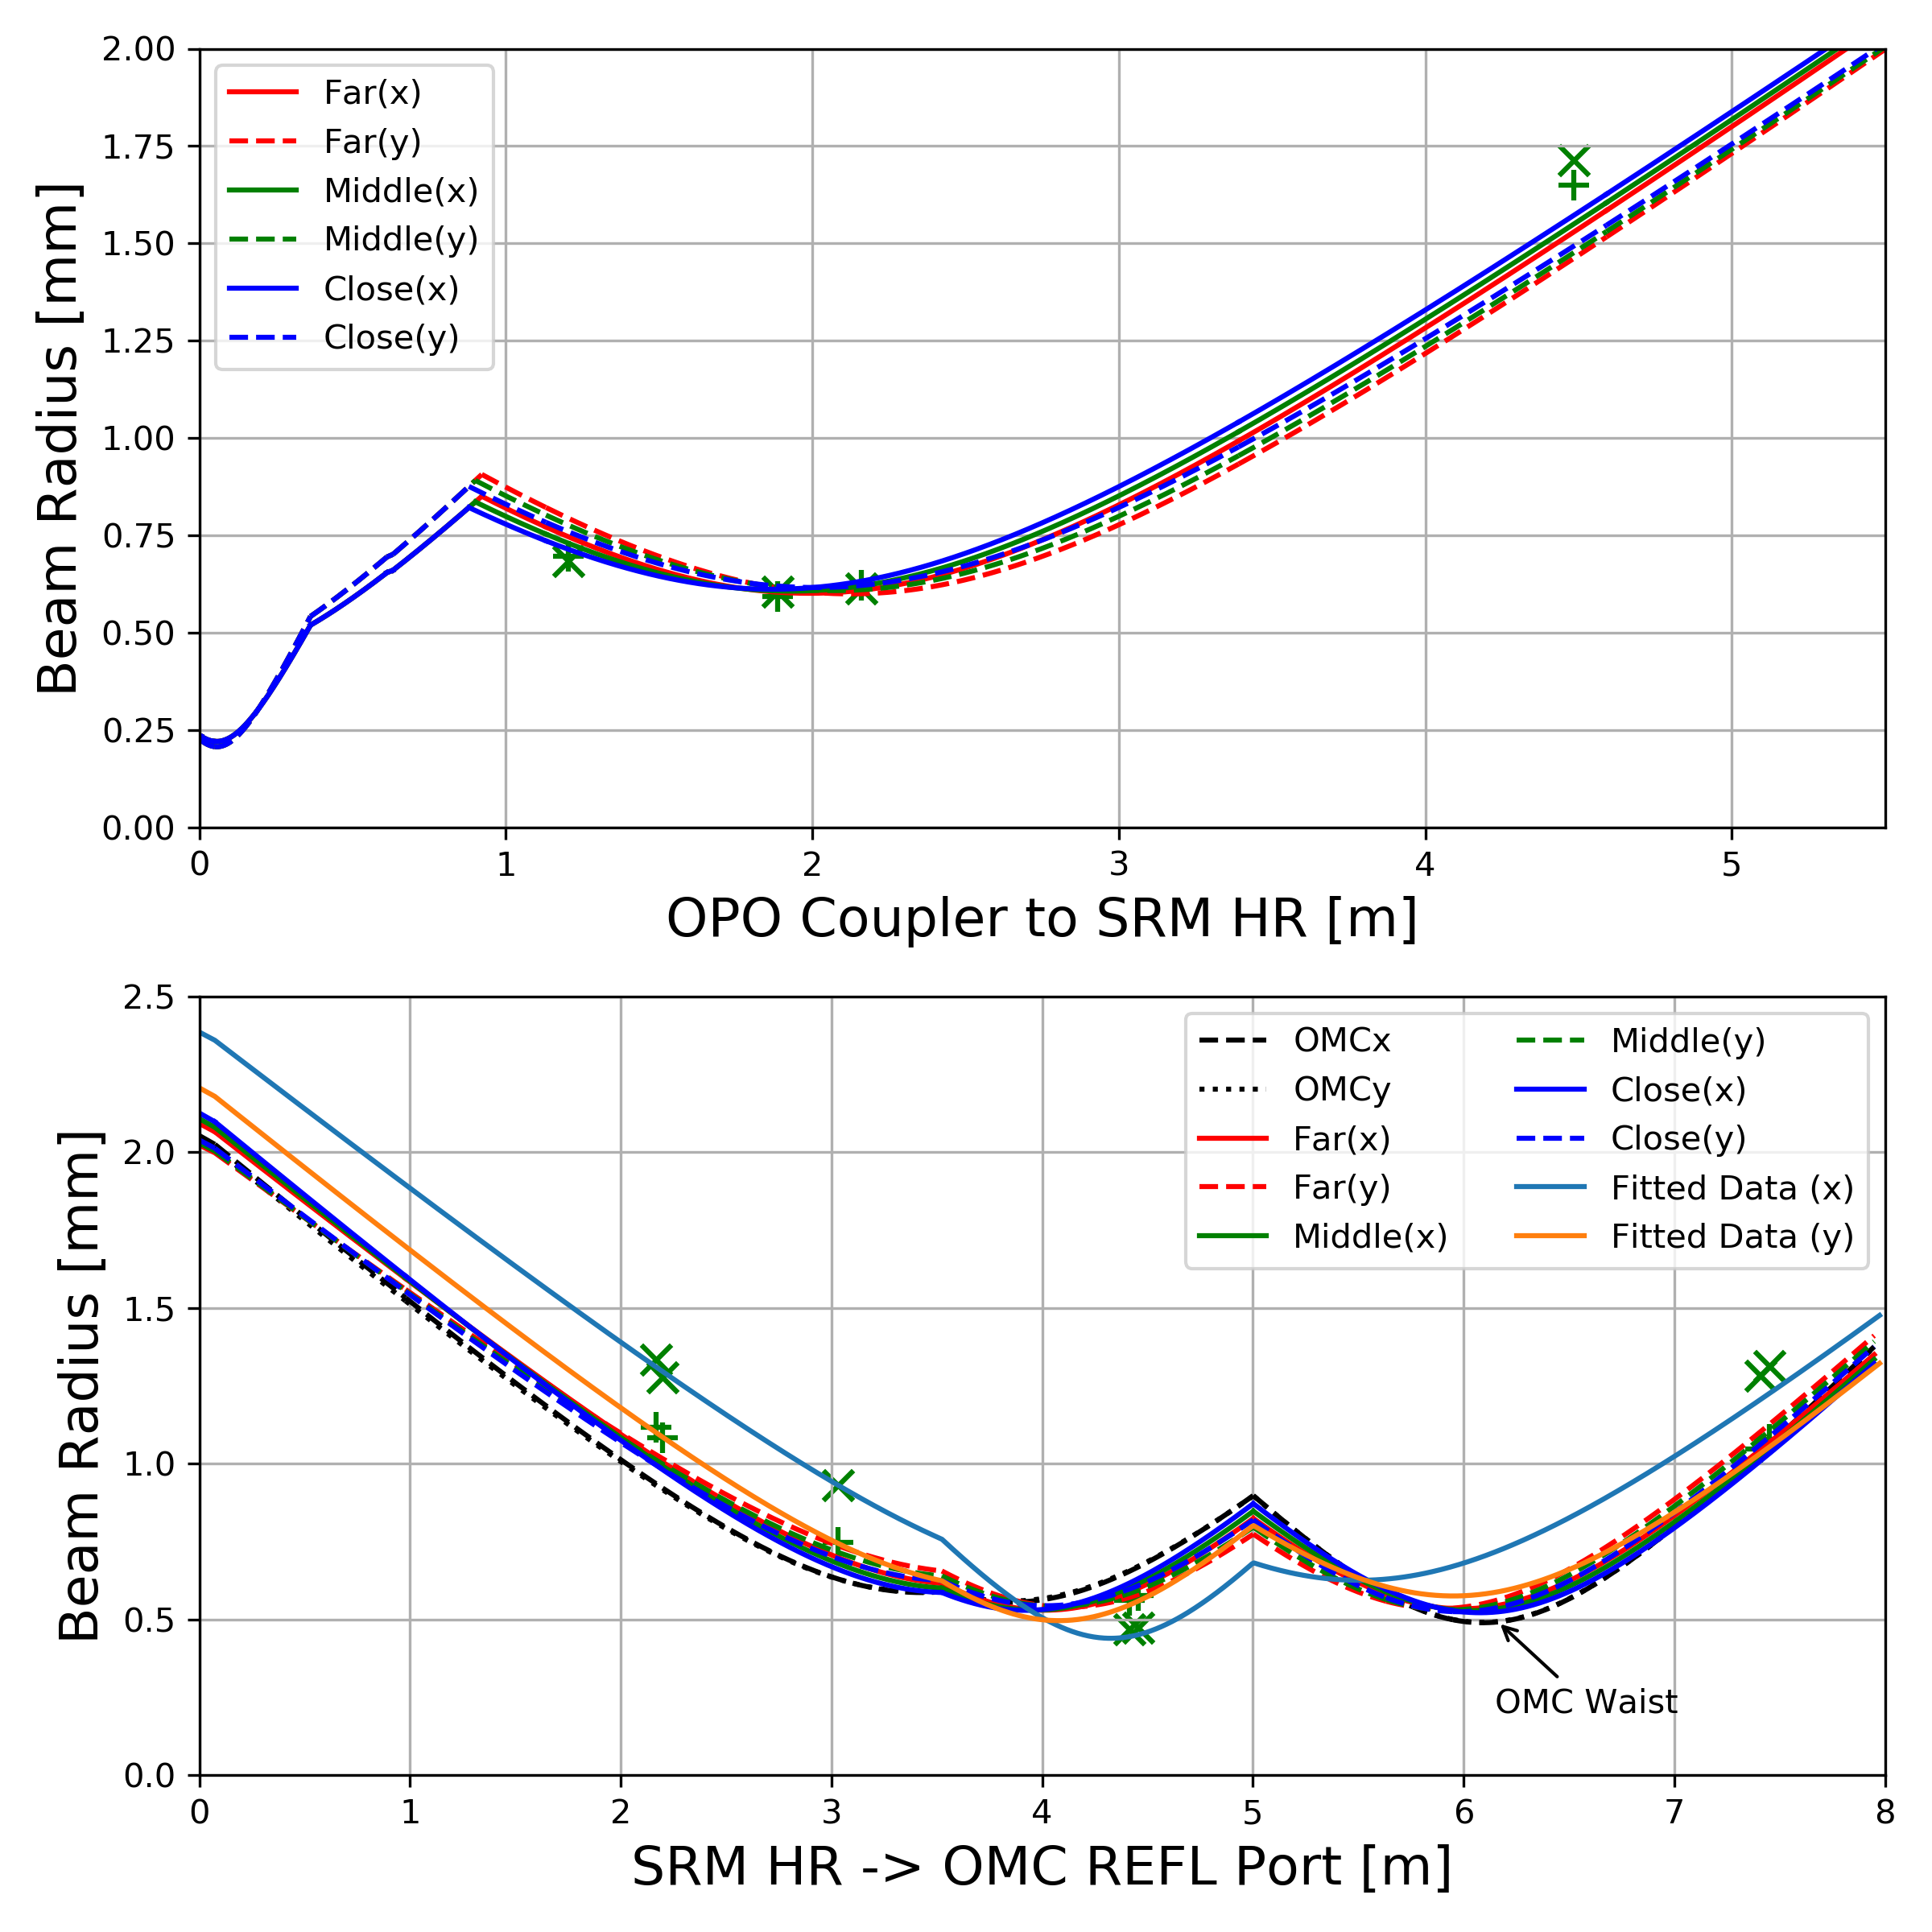
\includegraphics[width=0.8 \textwidth]{../Figures/OPO_to_OMCREFL_Newlenses.png}
	\caption[Repeated measurements with new lenses.]  
	{\textbf{Repeated measurements with new lenses.}  The model tries a few different lens solutions and settles on $f^{\text{new}}_{\text{Lens1}} = 250$ mm and $f_{\text{Lens2}} = 350$ mm, which severely limits the actuation range.  However, it shows approximately 97\% mode matching for the fitted transverse-y data and 92\% for the transverse-x data.  Astigmatism which was already shown in Figure \ref{fig:OPO_to_OMC_Old} is still prevalent here and brings the average mode matching to 95\% from the OPO to OMC in the single bounce configuration.
	}
	\label{fig:OPO_to_OMC_New}
	\end{figure}